\documentclass[twoside]{book}

% Packages required by doxygen
\usepackage{fixltx2e}
\usepackage{calc}
\usepackage{doxygen}
\usepackage[export]{adjustbox} % also loads graphicx
\usepackage{graphicx}
\usepackage[utf8]{inputenc}
\usepackage{makeidx}
\usepackage{multicol}
\usepackage{multirow}
\PassOptionsToPackage{warn}{textcomp}
\usepackage{textcomp}
\usepackage[nointegrals]{wasysym}
\usepackage[table]{xcolor}

% Font selection
\usepackage[T1]{fontenc}
\usepackage[scaled=.90]{helvet}
\usepackage{courier}
\usepackage{amssymb}
\usepackage{sectsty}
\renewcommand{\familydefault}{\sfdefault}
\allsectionsfont{%
  \fontseries{bc}\selectfont%
  \color{darkgray}%
}
\renewcommand{\DoxyLabelFont}{%
  \fontseries{bc}\selectfont%
  \color{darkgray}%
}
\newcommand{\+}{\discretionary{\mbox{\scriptsize$\hookleftarrow$}}{}{}}

% Page & text layout
\usepackage{geometry}
\geometry{%
  a4paper,%
  top=2.5cm,%
  bottom=2.5cm,%
  left=2.5cm,%
  right=2.5cm%
}
\tolerance=750
\hfuzz=15pt
\hbadness=750
\setlength{\emergencystretch}{15pt}
\setlength{\parindent}{0cm}
\setlength{\parskip}{3ex plus 2ex minus 2ex}
\makeatletter
\renewcommand{\paragraph}{%
  \@startsection{paragraph}{4}{0ex}{-1.0ex}{1.0ex}{%
    \normalfont\normalsize\bfseries\SS@parafont%
  }%
}
\renewcommand{\subparagraph}{%
  \@startsection{subparagraph}{5}{0ex}{-1.0ex}{1.0ex}{%
    \normalfont\normalsize\bfseries\SS@subparafont%
  }%
}
\makeatother

% Headers & footers
\usepackage{fancyhdr}
\pagestyle{fancyplain}
\fancyhead[LE]{\fancyplain{}{\bfseries\thepage}}
\fancyhead[CE]{\fancyplain{}{}}
\fancyhead[RE]{\fancyplain{}{\bfseries\leftmark}}
\fancyhead[LO]{\fancyplain{}{\bfseries\rightmark}}
\fancyhead[CO]{\fancyplain{}{}}
\fancyhead[RO]{\fancyplain{}{\bfseries\thepage}}
\fancyfoot[LE]{\fancyplain{}{}}
\fancyfoot[CE]{\fancyplain{}{}}
\fancyfoot[RE]{\fancyplain{}{\bfseries\scriptsize Generated by Doxygen }}
\fancyfoot[LO]{\fancyplain{}{\bfseries\scriptsize Generated by Doxygen }}
\fancyfoot[CO]{\fancyplain{}{}}
\fancyfoot[RO]{\fancyplain{}{}}
\renewcommand{\footrulewidth}{0.4pt}
\renewcommand{\chaptermark}[1]{%
  \markboth{#1}{}%
}
\renewcommand{\sectionmark}[1]{%
  \markright{\thesection\ #1}%
}

% Indices & bibliography
\usepackage{natbib}
\usepackage[titles]{tocloft}
\setcounter{tocdepth}{3}
\setcounter{secnumdepth}{5}
\makeindex

% Hyperlinks (required, but should be loaded last)
\usepackage{ifpdf}
\ifpdf
  \usepackage[pdftex,pagebackref=true]{hyperref}
\else
  \usepackage[ps2pdf,pagebackref=true]{hyperref}
\fi
\hypersetup{%
  colorlinks=true,%
  linkcolor=blue,%
  citecolor=blue,%
  unicode%
}

% Custom commands
\newcommand{\clearemptydoublepage}{%
  \newpage{\pagestyle{empty}\cleardoublepage}%
}

\usepackage{caption}
\captionsetup{labelsep=space,justification=centering,font={bf},singlelinecheck=off,skip=4pt,position=top}

%===== C O N T E N T S =====

\begin{document}

% Titlepage & ToC
\hypersetup{pageanchor=false,
             bookmarksnumbered=true,
             pdfencoding=unicode
            }
\pagenumbering{alph}
\begin{titlepage}
\vspace*{7cm}
\begin{center}%
{\Large Haru Engine }\\
\vspace*{1cm}
{\large Generated by Doxygen 1.8.14}\\
\end{center}
\end{titlepage}
\clearemptydoublepage
\pagenumbering{roman}
\tableofcontents
\clearemptydoublepage
\pagenumbering{arabic}
\hypersetup{pageanchor=true}

%--- Begin generated contents ---
\chapter{Namespace Index}
\section{Namespace List}
Here is a list of all namespaces with brief descriptions\+:\begin{DoxyCompactList}
\item\contentsline{section}{\mbox{\hyperlink{namespaceharu}{haru}} }{\pageref{namespaceharu}}{}
\end{DoxyCompactList}

\chapter{Hierarchical Index}
\section{Class Hierarchy}
This inheritance list is sorted roughly, but not completely, alphabetically\+:\begin{DoxyCompactList}
\item \contentsline{section}{haru\+:\+:Audio}{\pageref{classharu_1_1_audio}}{}
\item \contentsline{section}{haru\+:\+:Audio\+Impl}{\pageref{structharu_1_1_audio_impl}}{}
\item \contentsline{section}{Domain}{\pageref{class_domain}}{}
\item \contentsline{section}{haru\+:\+:E\+Screen}{\pageref{classharu_1_1_e_screen}}{}
\item exception\begin{DoxyCompactList}
\item \contentsline{section}{haru\+:\+:Exception}{\pageref{classharu_1_1_exception}}{}
\end{DoxyCompactList}
\item \contentsline{section}{haru\+:\+:Game\+Manager}{\pageref{classharu_1_1_game_manager}}{}
\item \contentsline{section}{Keyboard}{\pageref{class_keyboard}}{}
\item \contentsline{section}{haru\+:\+:Lighting}{\pageref{classharu_1_1_lighting}}{}
\item \contentsline{section}{haru\+:\+:Mouse}{\pageref{classharu_1_1_mouse}}{}
\item \contentsline{section}{haru\+:\+:Object}{\pageref{classharu_1_1_object}}{}
\item \contentsline{section}{haru\+:\+:Re\+Mesh}{\pageref{structharu_1_1_re_mesh}}{}
\item \contentsline{section}{haru\+:\+:Resource}{\pageref{classharu_1_1_resource}}{}
\item \contentsline{section}{haru\+:\+:Root}{\pageref{classharu_1_1_root}}{}
\item \contentsline{section}{haru\+:\+:Sampler}{\pageref{structharu_1_1_sampler}}{}
\item \contentsline{section}{haru\+:\+:Segment}{\pageref{classharu_1_1_segment}}{}
\begin{DoxyCompactList}
\item \contentsline{section}{haru\+:\+:Mesh\+Renderer}{\pageref{classharu_1_1_mesh_renderer}}{}
\end{DoxyCompactList}
\item \contentsline{section}{haru\+:\+:Shader\+Program}{\pageref{classharu_1_1_shader_program}}{}
\item \contentsline{section}{haru\+:\+:Texture}{\pageref{classharu_1_1_texture}}{}
\begin{DoxyCompactList}
\item \contentsline{section}{haru\+:\+:Render\+Texture}{\pageref{classharu_1_1_render_texture}}{}
\end{DoxyCompactList}
\item \contentsline{section}{haru\+:\+:Transform}{\pageref{classharu_1_1_transform}}{}
\item \contentsline{section}{haru\+:\+:Vertex\+Array}{\pageref{classharu_1_1_vertex_array}}{}
\item \contentsline{section}{haru\+:\+:Vertex\+Buffer}{\pageref{classharu_1_1_vertex_buffer}}{}
\end{DoxyCompactList}

\chapter{Class Index}
\section{Class List}
Here are the classes, structs, unions and interfaces with brief descriptions\+:\begin{DoxyCompactList}
\item\contentsline{section}{\mbox{\hyperlink{classharu_1_1_audio}{haru\+::\+Audio}} }{\pageref{classharu_1_1_audio}}{}
\item\contentsline{section}{\mbox{\hyperlink{structharu_1_1_audio_impl}{haru\+::\+Audio\+Impl}} }{\pageref{structharu_1_1_audio_impl}}{}
\item\contentsline{section}{\mbox{\hyperlink{class_domain}{Domain}} }{\pageref{class_domain}}{}
\item\contentsline{section}{\mbox{\hyperlink{classharu_1_1_e_screen}{haru\+::\+E\+Screen}} }{\pageref{classharu_1_1_e_screen}}{}
\item\contentsline{section}{\mbox{\hyperlink{classharu_1_1_exception}{haru\+::\+Exception}} }{\pageref{classharu_1_1_exception}}{}
\item\contentsline{section}{\mbox{\hyperlink{classharu_1_1_game_manager}{haru\+::\+Game\+Manager}} }{\pageref{classharu_1_1_game_manager}}{}
\item\contentsline{section}{\mbox{\hyperlink{class_keyboard}{Keyboard}} }{\pageref{class_keyboard}}{}
\item\contentsline{section}{\mbox{\hyperlink{classharu_1_1_lighting}{haru\+::\+Lighting}} }{\pageref{classharu_1_1_lighting}}{}
\item\contentsline{section}{\mbox{\hyperlink{classharu_1_1_mesh_renderer}{haru\+::\+Mesh\+Renderer}} }{\pageref{classharu_1_1_mesh_renderer}}{}
\item\contentsline{section}{\mbox{\hyperlink{classharu_1_1_mouse}{haru\+::\+Mouse}} }{\pageref{classharu_1_1_mouse}}{}
\item\contentsline{section}{\mbox{\hyperlink{classharu_1_1_object}{haru\+::\+Object}} }{\pageref{classharu_1_1_object}}{}
\item\contentsline{section}{\mbox{\hyperlink{structharu_1_1_re_mesh}{haru\+::\+Re\+Mesh}} }{\pageref{structharu_1_1_re_mesh}}{}
\item\contentsline{section}{\mbox{\hyperlink{classharu_1_1_render_texture}{haru\+::\+Render\+Texture}} }{\pageref{classharu_1_1_render_texture}}{}
\item\contentsline{section}{\mbox{\hyperlink{classharu_1_1_resource}{haru\+::\+Resource}} }{\pageref{classharu_1_1_resource}}{}
\item\contentsline{section}{\mbox{\hyperlink{classharu_1_1_root}{haru\+::\+Root}} }{\pageref{classharu_1_1_root}}{}
\item\contentsline{section}{\mbox{\hyperlink{structharu_1_1_sampler}{haru\+::\+Sampler}} }{\pageref{structharu_1_1_sampler}}{}
\item\contentsline{section}{\mbox{\hyperlink{classharu_1_1_segment}{haru\+::\+Segment}} }{\pageref{classharu_1_1_segment}}{}
\item\contentsline{section}{\mbox{\hyperlink{classharu_1_1_shader_program}{haru\+::\+Shader\+Program}} }{\pageref{classharu_1_1_shader_program}}{}
\item\contentsline{section}{\mbox{\hyperlink{classharu_1_1_texture}{haru\+::\+Texture}} }{\pageref{classharu_1_1_texture}}{}
\item\contentsline{section}{\mbox{\hyperlink{classharu_1_1_transform}{haru\+::\+Transform}} }{\pageref{classharu_1_1_transform}}{}
\item\contentsline{section}{\mbox{\hyperlink{classharu_1_1_vertex_array}{haru\+::\+Vertex\+Array}} }{\pageref{classharu_1_1_vertex_array}}{}
\item\contentsline{section}{\mbox{\hyperlink{classharu_1_1_vertex_buffer}{haru\+::\+Vertex\+Buffer}} }{\pageref{classharu_1_1_vertex_buffer}}{}
\end{DoxyCompactList}

\chapter{File Index}
\section{File List}
Here is a list of all files with brief descriptions\+:\begin{DoxyCompactList}
\item\contentsline{section}{source/game/\mbox{\hyperlink{main_8cpp}{main.\+cpp}} }{\pageref{main_8cpp}}{}
\item\contentsline{section}{source/haruengine/\mbox{\hyperlink{_audio_8cpp}{Audio.\+cpp}} }{\pageref{_audio_8cpp}}{}
\item\contentsline{section}{source/haruengine/\mbox{\hyperlink{_audio_8h}{Audio.\+h}} }{\pageref{_audio_8h}}{}
\item\contentsline{section}{source/haruengine/\mbox{\hyperlink{_domain_8cpp}{Domain.\+cpp}} }{\pageref{_domain_8cpp}}{}
\item\contentsline{section}{source/haruengine/\mbox{\hyperlink{_domain_8h}{Domain.\+h}} }{\pageref{_domain_8h}}{}
\item\contentsline{section}{source/haruengine/\mbox{\hyperlink{_e_screen_8cpp}{E\+Screen.\+cpp}} }{\pageref{_e_screen_8cpp}}{}
\item\contentsline{section}{source/haruengine/\mbox{\hyperlink{_e_screen_8h}{E\+Screen.\+h}} }{\pageref{_e_screen_8h}}{}
\item\contentsline{section}{source/haruengine/\mbox{\hyperlink{_exception_8cpp}{Exception.\+cpp}} }{\pageref{_exception_8cpp}}{}
\item\contentsline{section}{source/haruengine/\mbox{\hyperlink{_exception_8h}{Exception.\+h}} }{\pageref{_exception_8h}}{}
\item\contentsline{section}{source/haruengine/\mbox{\hyperlink{_game_manager_8cpp}{Game\+Manager.\+cpp}} }{\pageref{_game_manager_8cpp}}{}
\item\contentsline{section}{source/haruengine/\mbox{\hyperlink{_game_manager_8h}{Game\+Manager.\+h}} }{\pageref{_game_manager_8h}}{}
\item\contentsline{section}{source/haruengine/\mbox{\hyperlink{haru_8h}{haru.\+h}} }{\pageref{haru_8h}}{}
\item\contentsline{section}{source/haruengine/\mbox{\hyperlink{_keyboard_8cpp}{Keyboard.\+cpp}} }{\pageref{_keyboard_8cpp}}{}
\item\contentsline{section}{source/haruengine/\mbox{\hyperlink{_keyboard_8h}{Keyboard.\+h}} }{\pageref{_keyboard_8h}}{}
\item\contentsline{section}{source/haruengine/\mbox{\hyperlink{_lighting_8cpp}{Lighting.\+cpp}} }{\pageref{_lighting_8cpp}}{}
\item\contentsline{section}{source/haruengine/\mbox{\hyperlink{_lighting_8h}{Lighting.\+h}} }{\pageref{_lighting_8h}}{}
\item\contentsline{section}{source/haruengine/\mbox{\hyperlink{_mesh_8cpp}{Mesh.\+cpp}} }{\pageref{_mesh_8cpp}}{}
\item\contentsline{section}{source/haruengine/\mbox{\hyperlink{_mesh_8h}{Mesh.\+h}} }{\pageref{_mesh_8h}}{}
\item\contentsline{section}{source/haruengine/\mbox{\hyperlink{_mesh_renderer_8cpp}{Mesh\+Renderer.\+cpp}} }{\pageref{_mesh_renderer_8cpp}}{}
\item\contentsline{section}{source/haruengine/\mbox{\hyperlink{_mesh_renderer_8h}{Mesh\+Renderer.\+h}} }{\pageref{_mesh_renderer_8h}}{}
\item\contentsline{section}{source/haruengine/\mbox{\hyperlink{_mouse_8cpp}{Mouse.\+cpp}} }{\pageref{_mouse_8cpp}}{}
\item\contentsline{section}{source/haruengine/\mbox{\hyperlink{_mouse_8h}{Mouse.\+h}} }{\pageref{_mouse_8h}}{}
\item\contentsline{section}{source/haruengine/\mbox{\hyperlink{_object_8cpp}{Object.\+cpp}} }{\pageref{_object_8cpp}}{}
\item\contentsline{section}{source/haruengine/\mbox{\hyperlink{_object_8h}{Object.\+h}} }{\pageref{_object_8h}}{}
\item\contentsline{section}{source/haruengine/\mbox{\hyperlink{_render_texture_8cpp}{Render\+Texture.\+cpp}} }{\pageref{_render_texture_8cpp}}{}
\item\contentsline{section}{source/haruengine/\mbox{\hyperlink{_render_texture_8h}{Render\+Texture.\+h}} }{\pageref{_render_texture_8h}}{}
\item\contentsline{section}{source/haruengine/\mbox{\hyperlink{_resource_8cpp}{Resource.\+cpp}} }{\pageref{_resource_8cpp}}{}
\item\contentsline{section}{source/haruengine/\mbox{\hyperlink{_resource_8h}{Resource.\+h}} }{\pageref{_resource_8h}}{}
\item\contentsline{section}{source/haruengine/\mbox{\hyperlink{_root_8cpp}{Root.\+cpp}} }{\pageref{_root_8cpp}}{}
\item\contentsline{section}{source/haruengine/\mbox{\hyperlink{_root_8h}{Root.\+h}} }{\pageref{_root_8h}}{}
\item\contentsline{section}{source/haruengine/\mbox{\hyperlink{_segment_8cpp}{Segment.\+cpp}} }{\pageref{_segment_8cpp}}{}
\item\contentsline{section}{source/haruengine/\mbox{\hyperlink{_segment_8h}{Segment.\+h}} }{\pageref{_segment_8h}}{}
\item\contentsline{section}{source/haruengine/\mbox{\hyperlink{_shader_program_8cpp}{Shader\+Program.\+cpp}} }{\pageref{_shader_program_8cpp}}{}
\item\contentsline{section}{source/haruengine/\mbox{\hyperlink{_shader_program_8h}{Shader\+Program.\+h}} }{\pageref{_shader_program_8h}}{}
\item\contentsline{section}{source/haruengine/\mbox{\hyperlink{_texture_8cpp}{Texture.\+cpp}} }{\pageref{_texture_8cpp}}{}
\item\contentsline{section}{source/haruengine/\mbox{\hyperlink{_texture_8h}{Texture.\+h}} }{\pageref{_texture_8h}}{}
\item\contentsline{section}{source/haruengine/\mbox{\hyperlink{_transform_8cpp}{Transform.\+cpp}} }{\pageref{_transform_8cpp}}{}
\item\contentsline{section}{source/haruengine/\mbox{\hyperlink{_transform_8h}{Transform.\+h}} }{\pageref{_transform_8h}}{}
\item\contentsline{section}{source/haruengine/\mbox{\hyperlink{_vertex_array_8cpp}{Vertex\+Array.\+cpp}} }{\pageref{_vertex_array_8cpp}}{}
\item\contentsline{section}{source/haruengine/\mbox{\hyperlink{_vertex_array_8h}{Vertex\+Array.\+h}} }{\pageref{_vertex_array_8h}}{}
\item\contentsline{section}{source/haruengine/\mbox{\hyperlink{_vertex_buffer_8cpp}{Vertex\+Buffer.\+cpp}} }{\pageref{_vertex_buffer_8cpp}}{}
\item\contentsline{section}{source/haruengine/\mbox{\hyperlink{_vertex_buffer_8h}{Vertex\+Buffer.\+h}} }{\pageref{_vertex_buffer_8h}}{}
\end{DoxyCompactList}

\chapter{Namespace Documentation}
\hypertarget{namespaceharu}{}\section{haru Namespace Reference}
\label{namespaceharu}\index{haru@{haru}}
\subsection*{Classes}
\begin{DoxyCompactItemize}
\item 
class \mbox{\hyperlink{classharu_1_1_audio}{Audio}}
\item 
struct \mbox{\hyperlink{structharu_1_1_audio_impl}{Audio\+Impl}}
\item 
class \mbox{\hyperlink{classharu_1_1_e_screen}{E\+Screen}}
\item 
class \mbox{\hyperlink{classharu_1_1_exception}{Exception}}
\item 
class \mbox{\hyperlink{classharu_1_1_game_manager}{Game\+Manager}}
\item 
class \mbox{\hyperlink{classharu_1_1_lighting}{Lighting}}
\item 
class \mbox{\hyperlink{classharu_1_1_mesh_renderer}{Mesh\+Renderer}}
\item 
class \mbox{\hyperlink{classharu_1_1_mouse}{Mouse}}
\item 
class \mbox{\hyperlink{classharu_1_1_object}{Object}}
\item 
struct \mbox{\hyperlink{structharu_1_1_re_mesh}{Re\+Mesh}}
\item 
class \mbox{\hyperlink{classharu_1_1_render_texture}{Render\+Texture}}
\item 
class \mbox{\hyperlink{classharu_1_1_resource}{Resource}}
\item 
class \mbox{\hyperlink{classharu_1_1_root}{Root}}
\item 
struct \mbox{\hyperlink{structharu_1_1_sampler}{Sampler}}
\item 
class \mbox{\hyperlink{classharu_1_1_segment}{Segment}}
\item 
class \mbox{\hyperlink{classharu_1_1_shader_program}{Shader\+Program}}
\item 
class \mbox{\hyperlink{classharu_1_1_texture}{Texture}}
\item 
class \mbox{\hyperlink{classharu_1_1_transform}{Transform}}
\item 
class \mbox{\hyperlink{classharu_1_1_vertex_array}{Vertex\+Array}}
\item 
class \mbox{\hyperlink{classharu_1_1_vertex_buffer}{Vertex\+Buffer}}
\end{DoxyCompactItemize}

\chapter{Class Documentation}
\hypertarget{classharu_1_1_audio}{}\section{haru\+:\+:Audio Class Reference}
\label{classharu_1_1_audio}\index{haru\+::\+Audio@{haru\+::\+Audio}}


{\ttfamily \#include $<$Audio.\+h$>$}



Collaboration diagram for haru\+:\+:Audio\+:\nopagebreak
\begin{figure}[H]
\begin{center}
\leavevmode
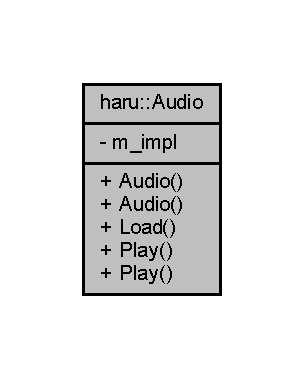
\includegraphics[width=146pt]{classharu_1_1_audio__coll__graph}
\end{center}
\end{figure}
\subsection*{Public Member Functions}
\begin{DoxyCompactItemize}
\item 
\mbox{\hyperlink{classharu_1_1_audio_aea8dbe76a9546e5caf2697d87e75d7db}{Audio}} ()
\item 
\mbox{\hyperlink{classharu_1_1_audio_ab1f431d428ad8f32a1fc3b0762ebb234}{Audio}} (std\+::string \+\_\+path)
\item 
void \mbox{\hyperlink{classharu_1_1_audio_a910757e64404e79e74f027189c56acd5}{Load}} (std\+::string \+\_\+path)
\item 
void \mbox{\hyperlink{classharu_1_1_audio_abedc73a31046f365320e7202d7c04b03}{Play}} ()
\item 
void \mbox{\hyperlink{classharu_1_1_audio_a0f9082d935880d64f4ee92493cfedf61}{Play}} (float \+\_\+vol, float \+\_\+var\+Min, float \+\_\+var\+Max)
\end{DoxyCompactItemize}
\subsection*{Private Attributes}
\begin{DoxyCompactItemize}
\item 
std\+::shared\+\_\+ptr$<$ \mbox{\hyperlink{structharu_1_1_audio_impl}{Audio\+Impl}} $>$ \mbox{\hyperlink{classharu_1_1_audio_a5118c3a3f1f33bcaee29dc619e3e68bd}{m\+\_\+impl}}
\end{DoxyCompactItemize}


\subsection{Constructor \& Destructor Documentation}
\mbox{\Hypertarget{classharu_1_1_audio_aea8dbe76a9546e5caf2697d87e75d7db}\label{classharu_1_1_audio_aea8dbe76a9546e5caf2697d87e75d7db}} 
\index{haru\+::\+Audio@{haru\+::\+Audio}!Audio@{Audio}}
\index{Audio@{Audio}!haru\+::\+Audio@{haru\+::\+Audio}}
\subsubsection{\texorpdfstring{Audio()}{Audio()}\hspace{0.1cm}{\footnotesize\ttfamily [1/2]}}
{\footnotesize\ttfamily haru\+::\+Audio\+::\+Audio (\begin{DoxyParamCaption}{ }\end{DoxyParamCaption})}

\mbox{\Hypertarget{classharu_1_1_audio_ab1f431d428ad8f32a1fc3b0762ebb234}\label{classharu_1_1_audio_ab1f431d428ad8f32a1fc3b0762ebb234}} 
\index{haru\+::\+Audio@{haru\+::\+Audio}!Audio@{Audio}}
\index{Audio@{Audio}!haru\+::\+Audio@{haru\+::\+Audio}}
\subsubsection{\texorpdfstring{Audio()}{Audio()}\hspace{0.1cm}{\footnotesize\ttfamily [2/2]}}
{\footnotesize\ttfamily haru\+::\+Audio\+::\+Audio (\begin{DoxyParamCaption}\item[{std\+::string}]{\+\_\+path }\end{DoxyParamCaption})}

Here is the call graph for this function\+:
\nopagebreak
\begin{figure}[H]
\begin{center}
\leavevmode
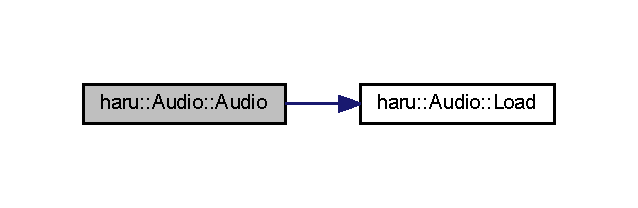
\includegraphics[width=306pt]{classharu_1_1_audio_ab1f431d428ad8f32a1fc3b0762ebb234_cgraph}
\end{center}
\end{figure}


\subsection{Member Function Documentation}
\mbox{\Hypertarget{classharu_1_1_audio_a910757e64404e79e74f027189c56acd5}\label{classharu_1_1_audio_a910757e64404e79e74f027189c56acd5}} 
\index{haru\+::\+Audio@{haru\+::\+Audio}!Load@{Load}}
\index{Load@{Load}!haru\+::\+Audio@{haru\+::\+Audio}}
\subsubsection{\texorpdfstring{Load()}{Load()}}
{\footnotesize\ttfamily void haru\+::\+Audio\+::\+Load (\begin{DoxyParamCaption}\item[{std\+::string}]{\+\_\+path }\end{DoxyParamCaption})}

Here is the caller graph for this function\+:
\nopagebreak
\begin{figure}[H]
\begin{center}
\leavevmode
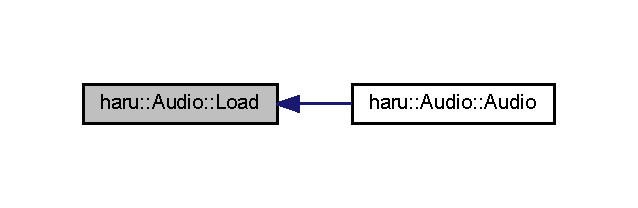
\includegraphics[width=306pt]{classharu_1_1_audio_a910757e64404e79e74f027189c56acd5_icgraph}
\end{center}
\end{figure}
\mbox{\Hypertarget{classharu_1_1_audio_abedc73a31046f365320e7202d7c04b03}\label{classharu_1_1_audio_abedc73a31046f365320e7202d7c04b03}} 
\index{haru\+::\+Audio@{haru\+::\+Audio}!Play@{Play}}
\index{Play@{Play}!haru\+::\+Audio@{haru\+::\+Audio}}
\subsubsection{\texorpdfstring{Play()}{Play()}\hspace{0.1cm}{\footnotesize\ttfamily [1/2]}}
{\footnotesize\ttfamily void haru\+::\+Audio\+::\+Play (\begin{DoxyParamCaption}{ }\end{DoxyParamCaption})}

\mbox{\Hypertarget{classharu_1_1_audio_a0f9082d935880d64f4ee92493cfedf61}\label{classharu_1_1_audio_a0f9082d935880d64f4ee92493cfedf61}} 
\index{haru\+::\+Audio@{haru\+::\+Audio}!Play@{Play}}
\index{Play@{Play}!haru\+::\+Audio@{haru\+::\+Audio}}
\subsubsection{\texorpdfstring{Play()}{Play()}\hspace{0.1cm}{\footnotesize\ttfamily [2/2]}}
{\footnotesize\ttfamily void haru\+::\+Audio\+::\+Play (\begin{DoxyParamCaption}\item[{float}]{\+\_\+vol,  }\item[{float}]{\+\_\+var\+Min,  }\item[{float}]{\+\_\+var\+Max }\end{DoxyParamCaption})}



\subsection{Member Data Documentation}
\mbox{\Hypertarget{classharu_1_1_audio_a5118c3a3f1f33bcaee29dc619e3e68bd}\label{classharu_1_1_audio_a5118c3a3f1f33bcaee29dc619e3e68bd}} 
\index{haru\+::\+Audio@{haru\+::\+Audio}!m\+\_\+impl@{m\+\_\+impl}}
\index{m\+\_\+impl@{m\+\_\+impl}!haru\+::\+Audio@{haru\+::\+Audio}}
\subsubsection{\texorpdfstring{m\+\_\+impl}{m\_impl}}
{\footnotesize\ttfamily std\+::shared\+\_\+ptr$<$\mbox{\hyperlink{structharu_1_1_audio_impl}{Audio\+Impl}}$>$ haru\+::\+Audio\+::m\+\_\+impl\hspace{0.3cm}{\ttfamily [private]}}



The documentation for this class was generated from the following files\+:\begin{DoxyCompactItemize}
\item 
source/haruengine/\mbox{\hyperlink{_audio_8h}{Audio.\+h}}\item 
source/haruengine/\mbox{\hyperlink{_audio_8cpp}{Audio.\+cpp}}\end{DoxyCompactItemize}

\hypertarget{structharu_1_1_audio_impl}{}\section{haru\+:\+:Audio\+Impl Struct Reference}
\label{structharu_1_1_audio_impl}\index{haru\+::\+Audio\+Impl@{haru\+::\+Audio\+Impl}}


Collaboration diagram for haru\+:\+:Audio\+Impl\+:\nopagebreak
\begin{figure}[H]
\begin{center}
\leavevmode
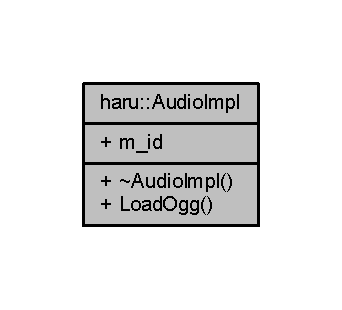
\includegraphics[width=164pt]{structharu_1_1_audio_impl__coll__graph}
\end{center}
\end{figure}
\subsection*{Public Member Functions}
\begin{DoxyCompactItemize}
\item 
\mbox{\hyperlink{structharu_1_1_audio_impl_a0504eaf0b1151dc0c42f7b5cd5e2f19a}{$\sim$\+Audio\+Impl}} ()
\item 
void \mbox{\hyperlink{structharu_1_1_audio_impl_a1bbcc60ff37aaf0e222210b82185a370}{Load\+Ogg}} (std\+::string \+\_\+file\+Name, std\+::vector$<$ char $>$ \&\+\_\+buffer, A\+Lenum \&\+\_\+format, A\+Lsizei \&\+\_\+freq)
\end{DoxyCompactItemize}
\subsection*{Public Attributes}
\begin{DoxyCompactItemize}
\item 
A\+Luint \mbox{\hyperlink{structharu_1_1_audio_impl_ac8e1bde9361d817cc1676c309cf6541a}{m\+\_\+id}}
\end{DoxyCompactItemize}


\subsection{Constructor \& Destructor Documentation}
\mbox{\Hypertarget{structharu_1_1_audio_impl_a0504eaf0b1151dc0c42f7b5cd5e2f19a}\label{structharu_1_1_audio_impl_a0504eaf0b1151dc0c42f7b5cd5e2f19a}} 
\index{haru\+::\+Audio\+Impl@{haru\+::\+Audio\+Impl}!````~Audio\+Impl@{$\sim$\+Audio\+Impl}}
\index{````~Audio\+Impl@{$\sim$\+Audio\+Impl}!haru\+::\+Audio\+Impl@{haru\+::\+Audio\+Impl}}
\subsubsection{\texorpdfstring{$\sim$\+Audio\+Impl()}{~AudioImpl()}}
{\footnotesize\ttfamily haru\+::\+Audio\+Impl\+::$\sim$\+Audio\+Impl (\begin{DoxyParamCaption}{ }\end{DoxyParamCaption})\hspace{0.3cm}{\ttfamily [inline]}}



\subsection{Member Function Documentation}
\mbox{\Hypertarget{structharu_1_1_audio_impl_a1bbcc60ff37aaf0e222210b82185a370}\label{structharu_1_1_audio_impl_a1bbcc60ff37aaf0e222210b82185a370}} 
\index{haru\+::\+Audio\+Impl@{haru\+::\+Audio\+Impl}!Load\+Ogg@{Load\+Ogg}}
\index{Load\+Ogg@{Load\+Ogg}!haru\+::\+Audio\+Impl@{haru\+::\+Audio\+Impl}}
\subsubsection{\texorpdfstring{Load\+Ogg()}{LoadOgg()}}
{\footnotesize\ttfamily void haru\+::\+Audio\+Impl\+::\+Load\+Ogg (\begin{DoxyParamCaption}\item[{std\+::string}]{\+\_\+file\+Name,  }\item[{std\+::vector$<$ char $>$ \&}]{\+\_\+buffer,  }\item[{A\+Lenum \&}]{\+\_\+format,  }\item[{A\+Lsizei \&}]{\+\_\+freq }\end{DoxyParamCaption})\hspace{0.3cm}{\ttfamily [inline]}}



\subsection{Member Data Documentation}
\mbox{\Hypertarget{structharu_1_1_audio_impl_ac8e1bde9361d817cc1676c309cf6541a}\label{structharu_1_1_audio_impl_ac8e1bde9361d817cc1676c309cf6541a}} 
\index{haru\+::\+Audio\+Impl@{haru\+::\+Audio\+Impl}!m\+\_\+id@{m\+\_\+id}}
\index{m\+\_\+id@{m\+\_\+id}!haru\+::\+Audio\+Impl@{haru\+::\+Audio\+Impl}}
\subsubsection{\texorpdfstring{m\+\_\+id}{m\_id}}
{\footnotesize\ttfamily A\+Luint haru\+::\+Audio\+Impl\+::m\+\_\+id}



The documentation for this struct was generated from the following file\+:\begin{DoxyCompactItemize}
\item 
source/haruengine/\mbox{\hyperlink{_audio_8cpp}{Audio.\+cpp}}\end{DoxyCompactItemize}

\hypertarget{class_domain}{}\section{Domain Class Reference}
\label{class_domain}\index{Domain@{Domain}}


{\ttfamily \#include $<$Domain.\+h$>$}



Collaboration diagram for Domain\+:\nopagebreak
\begin{figure}[H]
\begin{center}
\leavevmode
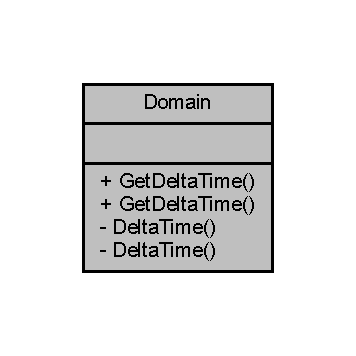
\includegraphics[width=171pt]{class_domain__coll__graph}
\end{center}
\end{figure}
\subsection*{Public Member Functions}
\begin{DoxyCompactItemize}
\item 
float \mbox{\hyperlink{class_domain_a595099f01805b1c9975a4d20be49e995}{Get\+Delta\+Time}} ()
\item 
float \mbox{\hyperlink{class_domain_a595099f01805b1c9975a4d20be49e995}{Get\+Delta\+Time}} ()
\end{DoxyCompactItemize}
\subsection*{Private Member Functions}
\begin{DoxyCompactItemize}
\item 
float \mbox{\hyperlink{class_domain_aba45357664ea3ca0566e079f229ad6a2}{Delta\+Time}} ()
\item 
float \mbox{\hyperlink{class_domain_aba45357664ea3ca0566e079f229ad6a2}{Delta\+Time}} ()
\end{DoxyCompactItemize}


\subsection{Member Function Documentation}
\mbox{\Hypertarget{class_domain_aba45357664ea3ca0566e079f229ad6a2}\label{class_domain_aba45357664ea3ca0566e079f229ad6a2}} 
\index{Domain@{Domain}!Delta\+Time@{Delta\+Time}}
\index{Delta\+Time@{Delta\+Time}!Domain@{Domain}}
\subsubsection{\texorpdfstring{Delta\+Time()}{DeltaTime()}\hspace{0.1cm}{\footnotesize\ttfamily [1/2]}}
{\footnotesize\ttfamily float Domain\+::\+Delta\+Time (\begin{DoxyParamCaption}{ }\end{DoxyParamCaption})\hspace{0.3cm}{\ttfamily [private]}}

\mbox{\Hypertarget{class_domain_aba45357664ea3ca0566e079f229ad6a2}\label{class_domain_aba45357664ea3ca0566e079f229ad6a2}} 
\index{Domain@{Domain}!Delta\+Time@{Delta\+Time}}
\index{Delta\+Time@{Delta\+Time}!Domain@{Domain}}
\subsubsection{\texorpdfstring{Delta\+Time()}{DeltaTime()}\hspace{0.1cm}{\footnotesize\ttfamily [2/2]}}
{\footnotesize\ttfamily float Domain\+::\+Delta\+Time (\begin{DoxyParamCaption}{ }\end{DoxyParamCaption})\hspace{0.3cm}{\ttfamily [private]}}

\mbox{\Hypertarget{class_domain_a595099f01805b1c9975a4d20be49e995}\label{class_domain_a595099f01805b1c9975a4d20be49e995}} 
\index{Domain@{Domain}!Get\+Delta\+Time@{Get\+Delta\+Time}}
\index{Get\+Delta\+Time@{Get\+Delta\+Time}!Domain@{Domain}}
\subsubsection{\texorpdfstring{Get\+Delta\+Time()}{GetDeltaTime()}\hspace{0.1cm}{\footnotesize\ttfamily [1/2]}}
{\footnotesize\ttfamily float Domain\+::\+Get\+Delta\+Time (\begin{DoxyParamCaption}{ }\end{DoxyParamCaption})}

\mbox{\Hypertarget{class_domain_a595099f01805b1c9975a4d20be49e995}\label{class_domain_a595099f01805b1c9975a4d20be49e995}} 
\index{Domain@{Domain}!Get\+Delta\+Time@{Get\+Delta\+Time}}
\index{Get\+Delta\+Time@{Get\+Delta\+Time}!Domain@{Domain}}
\subsubsection{\texorpdfstring{Get\+Delta\+Time()}{GetDeltaTime()}\hspace{0.1cm}{\footnotesize\ttfamily [2/2]}}
{\footnotesize\ttfamily float Domain\+::\+Get\+Delta\+Time (\begin{DoxyParamCaption}{ }\end{DoxyParamCaption})}



The documentation for this class was generated from the following files\+:\begin{DoxyCompactItemize}
\item 
source/haruengine/\mbox{\hyperlink{_domain_8h}{Domain.\+h}}\item 
source/haruengine/\mbox{\hyperlink{_mesh_8h}{Mesh.\+h}}\item 
source/haruengine/\mbox{\hyperlink{_domain_8cpp}{Domain.\+cpp}}\item 
source/haruengine/\mbox{\hyperlink{_mesh_8cpp}{Mesh.\+cpp}}\end{DoxyCompactItemize}

\hypertarget{classharu_1_1_e_screen}{}\section{haru\+:\+:E\+Screen Class Reference}
\label{classharu_1_1_e_screen}\index{haru\+::\+E\+Screen@{haru\+::\+E\+Screen}}


{\ttfamily \#include $<$E\+Screen.\+h$>$}



Collaboration diagram for haru\+:\+:E\+Screen\+:\nopagebreak
\begin{figure}[H]
\begin{center}
\leavevmode
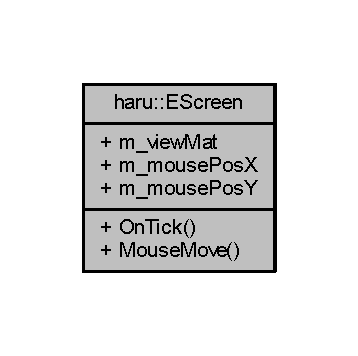
\includegraphics[width=172pt]{classharu_1_1_e_screen__coll__graph}
\end{center}
\end{figure}
\subsection*{Public Member Functions}
\begin{DoxyCompactItemize}
\item 
void \mbox{\hyperlink{classharu_1_1_e_screen_a600b05ce7a481cd681067d0fe311dd38}{On\+Tick}} ()
\item 
void \mbox{\hyperlink{classharu_1_1_e_screen_acdd8c57de946cbaf9e1658b2e4027367}{Mouse\+Move}} ()
\end{DoxyCompactItemize}
\subsection*{Public Attributes}
\begin{DoxyCompactItemize}
\item 
glm\+::mat4 \mbox{\hyperlink{classharu_1_1_e_screen_ac0d95afec2a766900d06e922978b5a72}{m\+\_\+view\+Mat}}
\item 
int \mbox{\hyperlink{classharu_1_1_e_screen_ac921a15804e3ca53a941b68bd4c67590}{m\+\_\+mouse\+PosX}}
\item 
int \mbox{\hyperlink{classharu_1_1_e_screen_ae53e4805bd5c7fcf49d33a7aa6fcf128}{m\+\_\+mouse\+PosY}}
\end{DoxyCompactItemize}


\subsection{Member Function Documentation}
\mbox{\Hypertarget{classharu_1_1_e_screen_acdd8c57de946cbaf9e1658b2e4027367}\label{classharu_1_1_e_screen_acdd8c57de946cbaf9e1658b2e4027367}} 
\index{haru\+::\+E\+Screen@{haru\+::\+E\+Screen}!Mouse\+Move@{Mouse\+Move}}
\index{Mouse\+Move@{Mouse\+Move}!haru\+::\+E\+Screen@{haru\+::\+E\+Screen}}
\subsubsection{\texorpdfstring{Mouse\+Move()}{MouseMove()}}
{\footnotesize\ttfamily void haru\+::\+E\+Screen\+::\+Mouse\+Move (\begin{DoxyParamCaption}{ }\end{DoxyParamCaption})}

\mbox{\Hypertarget{classharu_1_1_e_screen_a600b05ce7a481cd681067d0fe311dd38}\label{classharu_1_1_e_screen_a600b05ce7a481cd681067d0fe311dd38}} 
\index{haru\+::\+E\+Screen@{haru\+::\+E\+Screen}!On\+Tick@{On\+Tick}}
\index{On\+Tick@{On\+Tick}!haru\+::\+E\+Screen@{haru\+::\+E\+Screen}}
\subsubsection{\texorpdfstring{On\+Tick()}{OnTick()}}
{\footnotesize\ttfamily void haru\+::\+E\+Screen\+::\+On\+Tick (\begin{DoxyParamCaption}{ }\end{DoxyParamCaption})}



\subsection{Member Data Documentation}
\mbox{\Hypertarget{classharu_1_1_e_screen_ac921a15804e3ca53a941b68bd4c67590}\label{classharu_1_1_e_screen_ac921a15804e3ca53a941b68bd4c67590}} 
\index{haru\+::\+E\+Screen@{haru\+::\+E\+Screen}!m\+\_\+mouse\+PosX@{m\+\_\+mouse\+PosX}}
\index{m\+\_\+mouse\+PosX@{m\+\_\+mouse\+PosX}!haru\+::\+E\+Screen@{haru\+::\+E\+Screen}}
\subsubsection{\texorpdfstring{m\+\_\+mouse\+PosX}{m\_mousePosX}}
{\footnotesize\ttfamily int haru\+::\+E\+Screen\+::m\+\_\+mouse\+PosX}

\mbox{\Hypertarget{classharu_1_1_e_screen_ae53e4805bd5c7fcf49d33a7aa6fcf128}\label{classharu_1_1_e_screen_ae53e4805bd5c7fcf49d33a7aa6fcf128}} 
\index{haru\+::\+E\+Screen@{haru\+::\+E\+Screen}!m\+\_\+mouse\+PosY@{m\+\_\+mouse\+PosY}}
\index{m\+\_\+mouse\+PosY@{m\+\_\+mouse\+PosY}!haru\+::\+E\+Screen@{haru\+::\+E\+Screen}}
\subsubsection{\texorpdfstring{m\+\_\+mouse\+PosY}{m\_mousePosY}}
{\footnotesize\ttfamily int haru\+::\+E\+Screen\+::m\+\_\+mouse\+PosY}

\mbox{\Hypertarget{classharu_1_1_e_screen_ac0d95afec2a766900d06e922978b5a72}\label{classharu_1_1_e_screen_ac0d95afec2a766900d06e922978b5a72}} 
\index{haru\+::\+E\+Screen@{haru\+::\+E\+Screen}!m\+\_\+view\+Mat@{m\+\_\+view\+Mat}}
\index{m\+\_\+view\+Mat@{m\+\_\+view\+Mat}!haru\+::\+E\+Screen@{haru\+::\+E\+Screen}}
\subsubsection{\texorpdfstring{m\+\_\+view\+Mat}{m\_viewMat}}
{\footnotesize\ttfamily glm\+::mat4 haru\+::\+E\+Screen\+::m\+\_\+view\+Mat}



The documentation for this class was generated from the following files\+:\begin{DoxyCompactItemize}
\item 
source/haruengine/\mbox{\hyperlink{_e_screen_8h}{E\+Screen.\+h}}\item 
source/haruengine/\mbox{\hyperlink{_e_screen_8cpp}{E\+Screen.\+cpp}}\end{DoxyCompactItemize}

\hypertarget{classharu_1_1_exception}{}\section{haru\+:\+:Exception Class Reference}
\label{classharu_1_1_exception}\index{haru\+::\+Exception@{haru\+::\+Exception}}


{\ttfamily \#include $<$Exception.\+h$>$}



Inheritance diagram for haru\+:\+:Exception\+:\nopagebreak
\begin{figure}[H]
\begin{center}
\leavevmode
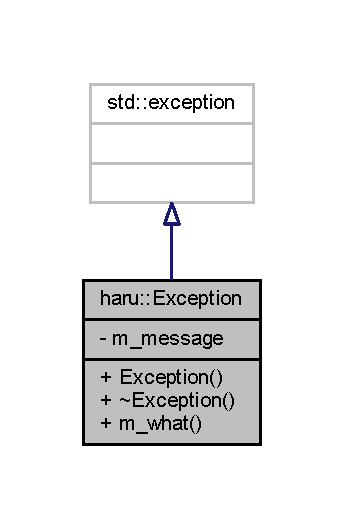
\includegraphics[width=165pt]{classharu_1_1_exception__inherit__graph}
\end{center}
\end{figure}


Collaboration diagram for haru\+:\+:Exception\+:\nopagebreak
\begin{figure}[H]
\begin{center}
\leavevmode
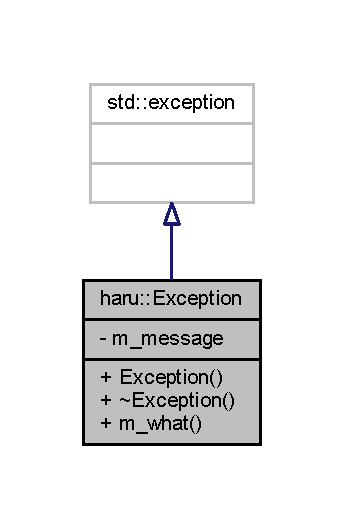
\includegraphics[width=165pt]{classharu_1_1_exception__coll__graph}
\end{center}
\end{figure}
\subsection*{Public Member Functions}
\begin{DoxyCompactItemize}
\item 
\mbox{\hyperlink{classharu_1_1_exception_a0bbb05d0c389c35b2917265a4d0fedfd}{Exception}} (std\+::string \+\_\+message)
\item 
\mbox{\hyperlink{classharu_1_1_exception_afcd6237b3d29ea8706f041a8d8f10ac9}{$\sim$\+Exception}} ()  throw ()
\item 
const char $\ast$ \mbox{\hyperlink{classharu_1_1_exception_a2b579cd90e5fcbf2894b903c3915550b}{m\+\_\+what}} () const noexcept
\end{DoxyCompactItemize}
\subsection*{Private Attributes}
\begin{DoxyCompactItemize}
\item 
std\+::string \mbox{\hyperlink{classharu_1_1_exception_a923972934d42b96a2af6f98668f757aa}{m\+\_\+message}}
\end{DoxyCompactItemize}


\subsection{Constructor \& Destructor Documentation}
\mbox{\Hypertarget{classharu_1_1_exception_a0bbb05d0c389c35b2917265a4d0fedfd}\label{classharu_1_1_exception_a0bbb05d0c389c35b2917265a4d0fedfd}} 
\index{haru\+::\+Exception@{haru\+::\+Exception}!Exception@{Exception}}
\index{Exception@{Exception}!haru\+::\+Exception@{haru\+::\+Exception}}
\subsubsection{\texorpdfstring{Exception()}{Exception()}}
{\footnotesize\ttfamily haru\+::\+Exception\+::\+Exception (\begin{DoxyParamCaption}\item[{std\+::string}]{\+\_\+message }\end{DoxyParamCaption})}

\mbox{\Hypertarget{classharu_1_1_exception_afcd6237b3d29ea8706f041a8d8f10ac9}\label{classharu_1_1_exception_afcd6237b3d29ea8706f041a8d8f10ac9}} 
\index{haru\+::\+Exception@{haru\+::\+Exception}!````~Exception@{$\sim$\+Exception}}
\index{````~Exception@{$\sim$\+Exception}!haru\+::\+Exception@{haru\+::\+Exception}}
\subsubsection{\texorpdfstring{$\sim$\+Exception()}{~Exception()}}
{\footnotesize\ttfamily haru\+::\+Exception\+::$\sim$\+Exception (\begin{DoxyParamCaption}{ }\end{DoxyParamCaption}) throw  ) }



\subsection{Member Function Documentation}
\mbox{\Hypertarget{classharu_1_1_exception_a2b579cd90e5fcbf2894b903c3915550b}\label{classharu_1_1_exception_a2b579cd90e5fcbf2894b903c3915550b}} 
\index{haru\+::\+Exception@{haru\+::\+Exception}!m\+\_\+what@{m\+\_\+what}}
\index{m\+\_\+what@{m\+\_\+what}!haru\+::\+Exception@{haru\+::\+Exception}}
\subsubsection{\texorpdfstring{m\+\_\+what()}{m\_what()}}
{\footnotesize\ttfamily const char$\ast$ haru\+::\+Exception\+::m\+\_\+what (\begin{DoxyParamCaption}{ }\end{DoxyParamCaption}) const\hspace{0.3cm}{\ttfamily [inline]}, {\ttfamily [noexcept]}}



\subsection{Member Data Documentation}
\mbox{\Hypertarget{classharu_1_1_exception_a923972934d42b96a2af6f98668f757aa}\label{classharu_1_1_exception_a923972934d42b96a2af6f98668f757aa}} 
\index{haru\+::\+Exception@{haru\+::\+Exception}!m\+\_\+message@{m\+\_\+message}}
\index{m\+\_\+message@{m\+\_\+message}!haru\+::\+Exception@{haru\+::\+Exception}}
\subsubsection{\texorpdfstring{m\+\_\+message}{m\_message}}
{\footnotesize\ttfamily std\+::string haru\+::\+Exception\+::m\+\_\+message\hspace{0.3cm}{\ttfamily [private]}}



The documentation for this class was generated from the following files\+:\begin{DoxyCompactItemize}
\item 
source/haruengine/\mbox{\hyperlink{_exception_8h}{Exception.\+h}}\item 
source/haruengine/\mbox{\hyperlink{_exception_8cpp}{Exception.\+cpp}}\end{DoxyCompactItemize}

\hypertarget{classharu_1_1_game_manager}{}\section{haru\+:\+:Game\+Manager Class Reference}
\label{classharu_1_1_game_manager}\index{haru\+::\+Game\+Manager@{haru\+::\+Game\+Manager}}


{\ttfamily \#include $<$Game\+Manager.\+h$>$}



Collaboration diagram for haru\+:\+:Game\+Manager\+:\nopagebreak
\begin{figure}[H]
\begin{center}
\leavevmode
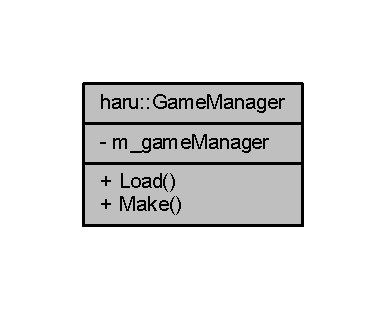
\includegraphics[width=185pt]{classharu_1_1_game_manager__coll__graph}
\end{center}
\end{figure}
\subsection*{Public Member Functions}
\begin{DoxyCompactItemize}
\item 
{\footnotesize template$<$typename T $>$ }\\std\+::shared\+\_\+ptr$<$ T $>$ \mbox{\hyperlink{classharu_1_1_game_manager_aa20022da42f771c1ff173f32570ed9b6}{Load}} (std\+::string \+\_\+path)
\item 
{\footnotesize template$<$typename T $>$ }\\std\+::shared\+\_\+ptr$<$ T $>$ \mbox{\hyperlink{classharu_1_1_game_manager_a447a6d9d5018fd8dcc0ab87f2ed4326d}{Make}} ()
\end{DoxyCompactItemize}
\subsection*{Private Attributes}
\begin{DoxyCompactItemize}
\item 
std\+::list$<$ std\+::shared\+\_\+ptr$<$ \mbox{\hyperlink{classharu_1_1_resource}{Resource}} $>$ $>$ \mbox{\hyperlink{classharu_1_1_game_manager_ab0183c1fa19eafb1448cc4e0a42e17c0}{m\+\_\+game\+Manager}}
\end{DoxyCompactItemize}


\subsection{Member Function Documentation}
\mbox{\Hypertarget{classharu_1_1_game_manager_aa20022da42f771c1ff173f32570ed9b6}\label{classharu_1_1_game_manager_aa20022da42f771c1ff173f32570ed9b6}} 
\index{haru\+::\+Game\+Manager@{haru\+::\+Game\+Manager}!Load@{Load}}
\index{Load@{Load}!haru\+::\+Game\+Manager@{haru\+::\+Game\+Manager}}
\subsubsection{\texorpdfstring{Load()}{Load()}}
{\footnotesize\ttfamily template$<$typename T $>$ \\
std\+::shared\+\_\+ptr$<$T$>$ haru\+::\+Game\+Manager\+::\+Load (\begin{DoxyParamCaption}\item[{std\+::string}]{\+\_\+path }\end{DoxyParamCaption})\hspace{0.3cm}{\ttfamily [inline]}}

\mbox{\Hypertarget{classharu_1_1_game_manager_a447a6d9d5018fd8dcc0ab87f2ed4326d}\label{classharu_1_1_game_manager_a447a6d9d5018fd8dcc0ab87f2ed4326d}} 
\index{haru\+::\+Game\+Manager@{haru\+::\+Game\+Manager}!Make@{Make}}
\index{Make@{Make}!haru\+::\+Game\+Manager@{haru\+::\+Game\+Manager}}
\subsubsection{\texorpdfstring{Make()}{Make()}}
{\footnotesize\ttfamily template$<$typename T $>$ \\
std\+::shared\+\_\+ptr$<$T$>$ haru\+::\+Game\+Manager\+::\+Make (\begin{DoxyParamCaption}{ }\end{DoxyParamCaption})\hspace{0.3cm}{\ttfamily [inline]}}



\subsection{Member Data Documentation}
\mbox{\Hypertarget{classharu_1_1_game_manager_ab0183c1fa19eafb1448cc4e0a42e17c0}\label{classharu_1_1_game_manager_ab0183c1fa19eafb1448cc4e0a42e17c0}} 
\index{haru\+::\+Game\+Manager@{haru\+::\+Game\+Manager}!m\+\_\+game\+Manager@{m\+\_\+game\+Manager}}
\index{m\+\_\+game\+Manager@{m\+\_\+game\+Manager}!haru\+::\+Game\+Manager@{haru\+::\+Game\+Manager}}
\subsubsection{\texorpdfstring{m\+\_\+game\+Manager}{m\_gameManager}}
{\footnotesize\ttfamily std\+::list$<$std\+::shared\+\_\+ptr$<$\mbox{\hyperlink{classharu_1_1_resource}{Resource}}$>$ $>$ haru\+::\+Game\+Manager\+::m\+\_\+game\+Manager\hspace{0.3cm}{\ttfamily [private]}}



The documentation for this class was generated from the following file\+:\begin{DoxyCompactItemize}
\item 
source/haruengine/\mbox{\hyperlink{_game_manager_8h}{Game\+Manager.\+h}}\end{DoxyCompactItemize}

\hypertarget{class_keyboard}{}\section{Keyboard Class Reference}
\label{class_keyboard}\index{Keyboard@{Keyboard}}


{\ttfamily \#include $<$Keyboard.\+h$>$}



Collaboration diagram for Keyboard\+:\nopagebreak
\begin{figure}[H]
\begin{center}
\leavevmode
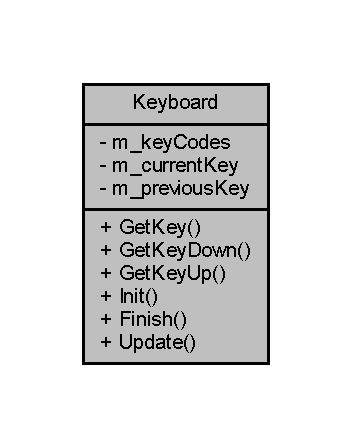
\includegraphics[width=169pt]{class_keyboard__coll__graph}
\end{center}
\end{figure}
\subsection*{Public Member Functions}
\begin{DoxyCompactItemize}
\item 
bool \mbox{\hyperlink{class_keyboard_a96e37d5e981c0a27e5839de9de9f91ee}{Get\+Key}} (int \+\_\+key\+Code)
\item 
bool \mbox{\hyperlink{class_keyboard_a1a10de35e37fa9a3300f2a71ef67e677}{Get\+Key\+Down}} (int \+\_\+key\+Code)
\item 
bool \mbox{\hyperlink{class_keyboard_a17da03653e9ea94b0175943fc317b56b}{Get\+Key\+Up}} (int \+\_\+key\+Code)
\item 
void \mbox{\hyperlink{class_keyboard_aa2ee7cfb4ef44e708877653a92af6f29}{Init}} ()
\item 
void \mbox{\hyperlink{class_keyboard_a817f09683a812ca7d2c737276e2b5dfa}{Finish}} ()
\item 
void \mbox{\hyperlink{class_keyboard_a071313d0ae6538e9307ff6a059aa9197}{Update}} ()
\end{DoxyCompactItemize}
\subsection*{Private Attributes}
\begin{DoxyCompactItemize}
\item 
int \mbox{\hyperlink{class_keyboard_a24b47a8a4639abfaca8347c6b16a5b4b}{m\+\_\+key\+Codes}}
\item 
Uint8 $\ast$ \mbox{\hyperlink{class_keyboard_ab8f8001628685fcda41978d5bdbb051d}{m\+\_\+current\+Key}}
\item 
Uint8 $\ast$ \mbox{\hyperlink{class_keyboard_a784ec6507f874cc67f12489fe0e6deeb}{m\+\_\+previous\+Key}}
\end{DoxyCompactItemize}


\subsection{Member Function Documentation}
\mbox{\Hypertarget{class_keyboard_a817f09683a812ca7d2c737276e2b5dfa}\label{class_keyboard_a817f09683a812ca7d2c737276e2b5dfa}} 
\index{Keyboard@{Keyboard}!Finish@{Finish}}
\index{Finish@{Finish}!Keyboard@{Keyboard}}
\subsubsection{\texorpdfstring{Finish()}{Finish()}}
{\footnotesize\ttfamily void Keyboard\+::\+Finish (\begin{DoxyParamCaption}{ }\end{DoxyParamCaption})}

\mbox{\Hypertarget{class_keyboard_a96e37d5e981c0a27e5839de9de9f91ee}\label{class_keyboard_a96e37d5e981c0a27e5839de9de9f91ee}} 
\index{Keyboard@{Keyboard}!Get\+Key@{Get\+Key}}
\index{Get\+Key@{Get\+Key}!Keyboard@{Keyboard}}
\subsubsection{\texorpdfstring{Get\+Key()}{GetKey()}}
{\footnotesize\ttfamily bool Keyboard\+::\+Get\+Key (\begin{DoxyParamCaption}\item[{int}]{\+\_\+key\+Code }\end{DoxyParamCaption})}

\mbox{\Hypertarget{class_keyboard_a1a10de35e37fa9a3300f2a71ef67e677}\label{class_keyboard_a1a10de35e37fa9a3300f2a71ef67e677}} 
\index{Keyboard@{Keyboard}!Get\+Key\+Down@{Get\+Key\+Down}}
\index{Get\+Key\+Down@{Get\+Key\+Down}!Keyboard@{Keyboard}}
\subsubsection{\texorpdfstring{Get\+Key\+Down()}{GetKeyDown()}}
{\footnotesize\ttfamily bool Keyboard\+::\+Get\+Key\+Down (\begin{DoxyParamCaption}\item[{int}]{\+\_\+key\+Code }\end{DoxyParamCaption})}

\mbox{\Hypertarget{class_keyboard_a17da03653e9ea94b0175943fc317b56b}\label{class_keyboard_a17da03653e9ea94b0175943fc317b56b}} 
\index{Keyboard@{Keyboard}!Get\+Key\+Up@{Get\+Key\+Up}}
\index{Get\+Key\+Up@{Get\+Key\+Up}!Keyboard@{Keyboard}}
\subsubsection{\texorpdfstring{Get\+Key\+Up()}{GetKeyUp()}}
{\footnotesize\ttfamily bool Keyboard\+::\+Get\+Key\+Up (\begin{DoxyParamCaption}\item[{int}]{\+\_\+key\+Code }\end{DoxyParamCaption})}

\mbox{\Hypertarget{class_keyboard_aa2ee7cfb4ef44e708877653a92af6f29}\label{class_keyboard_aa2ee7cfb4ef44e708877653a92af6f29}} 
\index{Keyboard@{Keyboard}!Init@{Init}}
\index{Init@{Init}!Keyboard@{Keyboard}}
\subsubsection{\texorpdfstring{Init()}{Init()}}
{\footnotesize\ttfamily void Keyboard\+::\+Init (\begin{DoxyParamCaption}{ }\end{DoxyParamCaption})}

\mbox{\Hypertarget{class_keyboard_a071313d0ae6538e9307ff6a059aa9197}\label{class_keyboard_a071313d0ae6538e9307ff6a059aa9197}} 
\index{Keyboard@{Keyboard}!Update@{Update}}
\index{Update@{Update}!Keyboard@{Keyboard}}
\subsubsection{\texorpdfstring{Update()}{Update()}}
{\footnotesize\ttfamily void Keyboard\+::\+Update (\begin{DoxyParamCaption}{ }\end{DoxyParamCaption})}



\subsection{Member Data Documentation}
\mbox{\Hypertarget{class_keyboard_ab8f8001628685fcda41978d5bdbb051d}\label{class_keyboard_ab8f8001628685fcda41978d5bdbb051d}} 
\index{Keyboard@{Keyboard}!m\+\_\+current\+Key@{m\+\_\+current\+Key}}
\index{m\+\_\+current\+Key@{m\+\_\+current\+Key}!Keyboard@{Keyboard}}
\subsubsection{\texorpdfstring{m\+\_\+current\+Key}{m\_currentKey}}
{\footnotesize\ttfamily Uint8$\ast$ Keyboard\+::m\+\_\+current\+Key\hspace{0.3cm}{\ttfamily [private]}}

\mbox{\Hypertarget{class_keyboard_a24b47a8a4639abfaca8347c6b16a5b4b}\label{class_keyboard_a24b47a8a4639abfaca8347c6b16a5b4b}} 
\index{Keyboard@{Keyboard}!m\+\_\+key\+Codes@{m\+\_\+key\+Codes}}
\index{m\+\_\+key\+Codes@{m\+\_\+key\+Codes}!Keyboard@{Keyboard}}
\subsubsection{\texorpdfstring{m\+\_\+key\+Codes}{m\_keyCodes}}
{\footnotesize\ttfamily int Keyboard\+::m\+\_\+key\+Codes\hspace{0.3cm}{\ttfamily [private]}}

\mbox{\Hypertarget{class_keyboard_a784ec6507f874cc67f12489fe0e6deeb}\label{class_keyboard_a784ec6507f874cc67f12489fe0e6deeb}} 
\index{Keyboard@{Keyboard}!m\+\_\+previous\+Key@{m\+\_\+previous\+Key}}
\index{m\+\_\+previous\+Key@{m\+\_\+previous\+Key}!Keyboard@{Keyboard}}
\subsubsection{\texorpdfstring{m\+\_\+previous\+Key}{m\_previousKey}}
{\footnotesize\ttfamily Uint8$\ast$ Keyboard\+::m\+\_\+previous\+Key\hspace{0.3cm}{\ttfamily [private]}}



The documentation for this class was generated from the following files\+:\begin{DoxyCompactItemize}
\item 
source/haruengine/\mbox{\hyperlink{_keyboard_8h}{Keyboard.\+h}}\item 
source/haruengine/\mbox{\hyperlink{_keyboard_8cpp}{Keyboard.\+cpp}}\end{DoxyCompactItemize}

\hypertarget{classharu_1_1_lighting}{}\section{haru\+:\+:Lighting Class Reference}
\label{classharu_1_1_lighting}\index{haru\+::\+Lighting@{haru\+::\+Lighting}}


{\ttfamily \#include $<$Lighting.\+h$>$}



Collaboration diagram for haru\+:\+:Lighting\+:\nopagebreak
\begin{figure}[H]
\begin{center}
\leavevmode
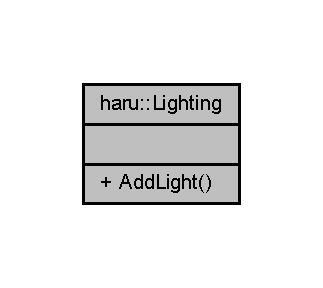
\includegraphics[width=155pt]{classharu_1_1_lighting__coll__graph}
\end{center}
\end{figure}
\subsection*{Public Member Functions}
\begin{DoxyCompactItemize}
\item 
void \mbox{\hyperlink{classharu_1_1_lighting_adeffec2cf38f48333986509af76df041}{Add\+Light}} ()
\end{DoxyCompactItemize}


\subsection{Member Function Documentation}
\mbox{\Hypertarget{classharu_1_1_lighting_adeffec2cf38f48333986509af76df041}\label{classharu_1_1_lighting_adeffec2cf38f48333986509af76df041}} 
\index{haru\+::\+Lighting@{haru\+::\+Lighting}!Add\+Light@{Add\+Light}}
\index{Add\+Light@{Add\+Light}!haru\+::\+Lighting@{haru\+::\+Lighting}}
\subsubsection{\texorpdfstring{Add\+Light()}{AddLight()}}
{\footnotesize\ttfamily void haru\+::\+Lighting\+::\+Add\+Light (\begin{DoxyParamCaption}{ }\end{DoxyParamCaption})}



The documentation for this class was generated from the following files\+:\begin{DoxyCompactItemize}
\item 
source/haruengine/\mbox{\hyperlink{_lighting_8h}{Lighting.\+h}}\item 
source/haruengine/\mbox{\hyperlink{_lighting_8cpp}{Lighting.\+cpp}}\end{DoxyCompactItemize}

\hypertarget{classharu_1_1_mesh_renderer}{}\section{haru\+:\+:Mesh\+Renderer Class Reference}
\label{classharu_1_1_mesh_renderer}\index{haru\+::\+Mesh\+Renderer@{haru\+::\+Mesh\+Renderer}}


{\ttfamily \#include $<$Mesh\+Renderer.\+h$>$}



Inheritance diagram for haru\+:\+:Mesh\+Renderer\+:\nopagebreak
\begin{figure}[H]
\begin{center}
\leavevmode
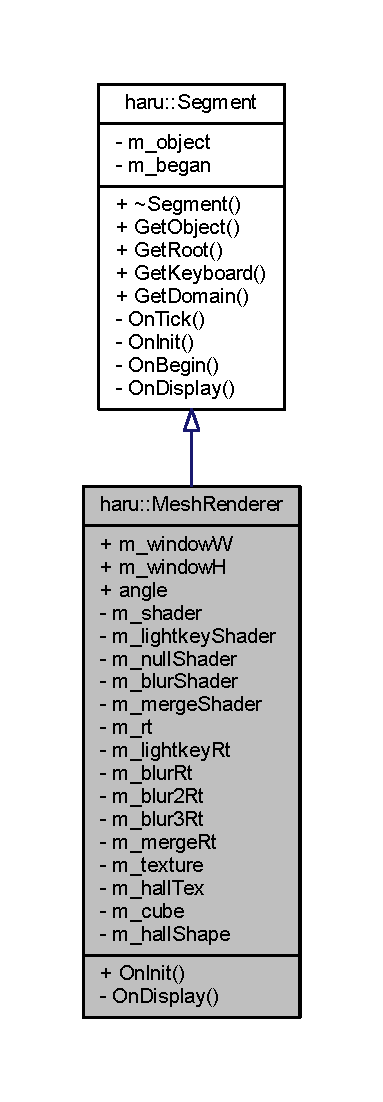
\includegraphics[width=184pt]{classharu_1_1_mesh_renderer__inherit__graph}
\end{center}
\end{figure}


Collaboration diagram for haru\+:\+:Mesh\+Renderer\+:\nopagebreak
\begin{figure}[H]
\begin{center}
\leavevmode
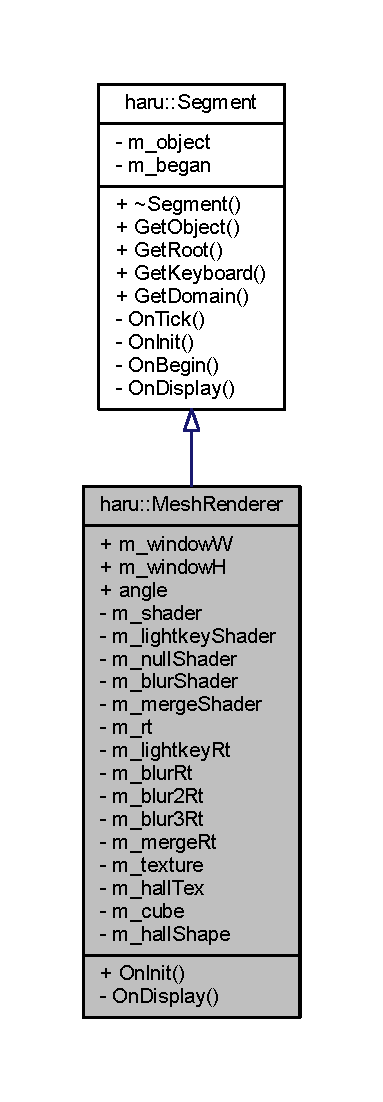
\includegraphics[width=184pt]{classharu_1_1_mesh_renderer__coll__graph}
\end{center}
\end{figure}
\subsection*{Public Member Functions}
\begin{DoxyCompactItemize}
\item 
void \mbox{\hyperlink{classharu_1_1_mesh_renderer_a5a6a5b945fc7560d166e9d16058aec53}{On\+Init}} ()
\end{DoxyCompactItemize}
\subsection*{Public Attributes}
\begin{DoxyCompactItemize}
\item 
int \mbox{\hyperlink{classharu_1_1_mesh_renderer_a30ea5ddf109ff42564c5eecfb73d4b4f}{m\+\_\+windowW}} = 800
\item 
int \mbox{\hyperlink{classharu_1_1_mesh_renderer_a17e10695dd67e9094bd28c110231082c}{m\+\_\+windowH}} = 800
\item 
float \mbox{\hyperlink{classharu_1_1_mesh_renderer_ad1881dc8b63b1824fadc85436624241c}{angle}} = 0
\end{DoxyCompactItemize}
\subsection*{Private Member Functions}
\begin{DoxyCompactItemize}
\item 
void \mbox{\hyperlink{classharu_1_1_mesh_renderer_ac927c9cc1d392ca8305ca995ddc0b7a6}{On\+Display}} ()
\end{DoxyCompactItemize}
\subsection*{Private Attributes}
\begin{DoxyCompactItemize}
\item 
std\+::shared\+\_\+ptr$<$ \mbox{\hyperlink{classharu_1_1_shader_program}{Shader\+Program}} $>$ \mbox{\hyperlink{classharu_1_1_mesh_renderer_a362bf54c45c36b194f1421ffc154f034}{m\+\_\+shader}}
\item 
std\+::shared\+\_\+ptr$<$ \mbox{\hyperlink{classharu_1_1_shader_program}{Shader\+Program}} $>$ \mbox{\hyperlink{classharu_1_1_mesh_renderer_a1b7b13260f00ea7e57df2d7c78c862bc}{m\+\_\+lightkey\+Shader}}
\item 
std\+::shared\+\_\+ptr$<$ \mbox{\hyperlink{classharu_1_1_shader_program}{Shader\+Program}} $>$ \mbox{\hyperlink{classharu_1_1_mesh_renderer_a08d71f5b79e9292aa3123443a4daa621}{m\+\_\+null\+Shader}}
\item 
std\+::shared\+\_\+ptr$<$ \mbox{\hyperlink{classharu_1_1_shader_program}{Shader\+Program}} $>$ \mbox{\hyperlink{classharu_1_1_mesh_renderer_afcc5562d658a94ec8905e590e9a41973}{m\+\_\+blur\+Shader}}
\item 
std\+::shared\+\_\+ptr$<$ \mbox{\hyperlink{classharu_1_1_shader_program}{Shader\+Program}} $>$ \mbox{\hyperlink{classharu_1_1_mesh_renderer_ae91deec127f7cf0093a6bf99e97f9bba}{m\+\_\+merge\+Shader}}
\item 
std\+::shared\+\_\+ptr$<$ \mbox{\hyperlink{classharu_1_1_render_texture}{Render\+Texture}} $>$ \mbox{\hyperlink{classharu_1_1_mesh_renderer_acf20639ec4df5f7aec8324c53d9cea6b}{m\+\_\+rt}}
\item 
std\+::shared\+\_\+ptr$<$ \mbox{\hyperlink{classharu_1_1_render_texture}{Render\+Texture}} $>$ \mbox{\hyperlink{classharu_1_1_mesh_renderer_a933fb51943b65589f92e0c750d4e0e9e}{m\+\_\+lightkey\+Rt}}
\item 
std\+::shared\+\_\+ptr$<$ \mbox{\hyperlink{classharu_1_1_render_texture}{Render\+Texture}} $>$ \mbox{\hyperlink{classharu_1_1_mesh_renderer_af06d5e4929335a9681cb87cdb1a4537a}{m\+\_\+blur\+Rt}}
\item 
std\+::shared\+\_\+ptr$<$ \mbox{\hyperlink{classharu_1_1_render_texture}{Render\+Texture}} $>$ \mbox{\hyperlink{classharu_1_1_mesh_renderer_a7e980792681d9b28915b27f46dfa99ac}{m\+\_\+blur2\+Rt}}
\item 
std\+::shared\+\_\+ptr$<$ \mbox{\hyperlink{classharu_1_1_render_texture}{Render\+Texture}} $>$ \mbox{\hyperlink{classharu_1_1_mesh_renderer_a457ee3e43f876531601198f3a2a11363}{m\+\_\+blur3\+Rt}}
\item 
std\+::shared\+\_\+ptr$<$ \mbox{\hyperlink{classharu_1_1_render_texture}{Render\+Texture}} $>$ \mbox{\hyperlink{classharu_1_1_mesh_renderer_a5cfa897f6d0aeb687f1b6e091c6c079e}{m\+\_\+merge\+Rt}}
\item 
std\+::shared\+\_\+ptr$<$ \mbox{\hyperlink{classharu_1_1_texture}{Texture}} $>$ \mbox{\hyperlink{classharu_1_1_mesh_renderer_abea78715a7752ce3ea0311f89ffcbbc9}{m\+\_\+texture}}
\item 
std\+::shared\+\_\+ptr$<$ \mbox{\hyperlink{classharu_1_1_texture}{Texture}} $>$ \mbox{\hyperlink{classharu_1_1_mesh_renderer_a9c59297b0cbcc1e13adfdebbb6edcdcd}{m\+\_\+hall\+Tex}}
\item 
std\+::shared\+\_\+ptr$<$ \mbox{\hyperlink{classharu_1_1_vertex_array}{Vertex\+Array}} $>$ \mbox{\hyperlink{classharu_1_1_mesh_renderer_a8911a9066c7d9ddbf87126d5dccb2246}{m\+\_\+cube}}
\item 
std\+::shared\+\_\+ptr$<$ \mbox{\hyperlink{classharu_1_1_vertex_array}{Vertex\+Array}} $>$ \mbox{\hyperlink{classharu_1_1_mesh_renderer_a84b8747803ab80c6b1f827f7c8c2ac5a}{m\+\_\+hall\+Shape}}
\end{DoxyCompactItemize}


\subsection{Member Function Documentation}
\mbox{\Hypertarget{classharu_1_1_mesh_renderer_ac927c9cc1d392ca8305ca995ddc0b7a6}\label{classharu_1_1_mesh_renderer_ac927c9cc1d392ca8305ca995ddc0b7a6}} 
\index{haru\+::\+Mesh\+Renderer@{haru\+::\+Mesh\+Renderer}!On\+Display@{On\+Display}}
\index{On\+Display@{On\+Display}!haru\+::\+Mesh\+Renderer@{haru\+::\+Mesh\+Renderer}}
\subsubsection{\texorpdfstring{On\+Display()}{OnDisplay()}}
{\footnotesize\ttfamily void haru\+::\+Mesh\+Renderer\+::\+On\+Display (\begin{DoxyParamCaption}{ }\end{DoxyParamCaption})\hspace{0.3cm}{\ttfamily [private]}, {\ttfamily [virtual]}}



Reimplemented from \mbox{\hyperlink{classharu_1_1_segment_a5bb0f5cf9aecda465804016d3ed4092c}{haru\+::\+Segment}}.

\mbox{\Hypertarget{classharu_1_1_mesh_renderer_a5a6a5b945fc7560d166e9d16058aec53}\label{classharu_1_1_mesh_renderer_a5a6a5b945fc7560d166e9d16058aec53}} 
\index{haru\+::\+Mesh\+Renderer@{haru\+::\+Mesh\+Renderer}!On\+Init@{On\+Init}}
\index{On\+Init@{On\+Init}!haru\+::\+Mesh\+Renderer@{haru\+::\+Mesh\+Renderer}}
\subsubsection{\texorpdfstring{On\+Init()}{OnInit()}}
{\footnotesize\ttfamily void haru\+::\+Mesh\+Renderer\+::\+On\+Init (\begin{DoxyParamCaption}{ }\end{DoxyParamCaption})\hspace{0.3cm}{\ttfamily [virtual]}}



Reimplemented from \mbox{\hyperlink{classharu_1_1_segment_adc41c8e5769e0057ade94abf669c6dbc}{haru\+::\+Segment}}.



\subsection{Member Data Documentation}
\mbox{\Hypertarget{classharu_1_1_mesh_renderer_ad1881dc8b63b1824fadc85436624241c}\label{classharu_1_1_mesh_renderer_ad1881dc8b63b1824fadc85436624241c}} 
\index{haru\+::\+Mesh\+Renderer@{haru\+::\+Mesh\+Renderer}!angle@{angle}}
\index{angle@{angle}!haru\+::\+Mesh\+Renderer@{haru\+::\+Mesh\+Renderer}}
\subsubsection{\texorpdfstring{angle}{angle}}
{\footnotesize\ttfamily float haru\+::\+Mesh\+Renderer\+::angle = 0}

\mbox{\Hypertarget{classharu_1_1_mesh_renderer_a7e980792681d9b28915b27f46dfa99ac}\label{classharu_1_1_mesh_renderer_a7e980792681d9b28915b27f46dfa99ac}} 
\index{haru\+::\+Mesh\+Renderer@{haru\+::\+Mesh\+Renderer}!m\+\_\+blur2\+Rt@{m\+\_\+blur2\+Rt}}
\index{m\+\_\+blur2\+Rt@{m\+\_\+blur2\+Rt}!haru\+::\+Mesh\+Renderer@{haru\+::\+Mesh\+Renderer}}
\subsubsection{\texorpdfstring{m\+\_\+blur2\+Rt}{m\_blur2Rt}}
{\footnotesize\ttfamily std\+::shared\+\_\+ptr$<$\mbox{\hyperlink{classharu_1_1_render_texture}{Render\+Texture}}$>$ haru\+::\+Mesh\+Renderer\+::m\+\_\+blur2\+Rt\hspace{0.3cm}{\ttfamily [private]}}

\mbox{\Hypertarget{classharu_1_1_mesh_renderer_a457ee3e43f876531601198f3a2a11363}\label{classharu_1_1_mesh_renderer_a457ee3e43f876531601198f3a2a11363}} 
\index{haru\+::\+Mesh\+Renderer@{haru\+::\+Mesh\+Renderer}!m\+\_\+blur3\+Rt@{m\+\_\+blur3\+Rt}}
\index{m\+\_\+blur3\+Rt@{m\+\_\+blur3\+Rt}!haru\+::\+Mesh\+Renderer@{haru\+::\+Mesh\+Renderer}}
\subsubsection{\texorpdfstring{m\+\_\+blur3\+Rt}{m\_blur3Rt}}
{\footnotesize\ttfamily std\+::shared\+\_\+ptr$<$\mbox{\hyperlink{classharu_1_1_render_texture}{Render\+Texture}}$>$ haru\+::\+Mesh\+Renderer\+::m\+\_\+blur3\+Rt\hspace{0.3cm}{\ttfamily [private]}}

\mbox{\Hypertarget{classharu_1_1_mesh_renderer_af06d5e4929335a9681cb87cdb1a4537a}\label{classharu_1_1_mesh_renderer_af06d5e4929335a9681cb87cdb1a4537a}} 
\index{haru\+::\+Mesh\+Renderer@{haru\+::\+Mesh\+Renderer}!m\+\_\+blur\+Rt@{m\+\_\+blur\+Rt}}
\index{m\+\_\+blur\+Rt@{m\+\_\+blur\+Rt}!haru\+::\+Mesh\+Renderer@{haru\+::\+Mesh\+Renderer}}
\subsubsection{\texorpdfstring{m\+\_\+blur\+Rt}{m\_blurRt}}
{\footnotesize\ttfamily std\+::shared\+\_\+ptr$<$\mbox{\hyperlink{classharu_1_1_render_texture}{Render\+Texture}}$>$ haru\+::\+Mesh\+Renderer\+::m\+\_\+blur\+Rt\hspace{0.3cm}{\ttfamily [private]}}

\mbox{\Hypertarget{classharu_1_1_mesh_renderer_afcc5562d658a94ec8905e590e9a41973}\label{classharu_1_1_mesh_renderer_afcc5562d658a94ec8905e590e9a41973}} 
\index{haru\+::\+Mesh\+Renderer@{haru\+::\+Mesh\+Renderer}!m\+\_\+blur\+Shader@{m\+\_\+blur\+Shader}}
\index{m\+\_\+blur\+Shader@{m\+\_\+blur\+Shader}!haru\+::\+Mesh\+Renderer@{haru\+::\+Mesh\+Renderer}}
\subsubsection{\texorpdfstring{m\+\_\+blur\+Shader}{m\_blurShader}}
{\footnotesize\ttfamily std\+::shared\+\_\+ptr$<$\mbox{\hyperlink{classharu_1_1_shader_program}{Shader\+Program}}$>$ haru\+::\+Mesh\+Renderer\+::m\+\_\+blur\+Shader\hspace{0.3cm}{\ttfamily [private]}}

\mbox{\Hypertarget{classharu_1_1_mesh_renderer_a8911a9066c7d9ddbf87126d5dccb2246}\label{classharu_1_1_mesh_renderer_a8911a9066c7d9ddbf87126d5dccb2246}} 
\index{haru\+::\+Mesh\+Renderer@{haru\+::\+Mesh\+Renderer}!m\+\_\+cube@{m\+\_\+cube}}
\index{m\+\_\+cube@{m\+\_\+cube}!haru\+::\+Mesh\+Renderer@{haru\+::\+Mesh\+Renderer}}
\subsubsection{\texorpdfstring{m\+\_\+cube}{m\_cube}}
{\footnotesize\ttfamily std\+::shared\+\_\+ptr$<$\mbox{\hyperlink{classharu_1_1_vertex_array}{Vertex\+Array}}$>$ haru\+::\+Mesh\+Renderer\+::m\+\_\+cube\hspace{0.3cm}{\ttfamily [private]}}

\mbox{\Hypertarget{classharu_1_1_mesh_renderer_a84b8747803ab80c6b1f827f7c8c2ac5a}\label{classharu_1_1_mesh_renderer_a84b8747803ab80c6b1f827f7c8c2ac5a}} 
\index{haru\+::\+Mesh\+Renderer@{haru\+::\+Mesh\+Renderer}!m\+\_\+hall\+Shape@{m\+\_\+hall\+Shape}}
\index{m\+\_\+hall\+Shape@{m\+\_\+hall\+Shape}!haru\+::\+Mesh\+Renderer@{haru\+::\+Mesh\+Renderer}}
\subsubsection{\texorpdfstring{m\+\_\+hall\+Shape}{m\_hallShape}}
{\footnotesize\ttfamily std\+::shared\+\_\+ptr$<$\mbox{\hyperlink{classharu_1_1_vertex_array}{Vertex\+Array}}$>$ haru\+::\+Mesh\+Renderer\+::m\+\_\+hall\+Shape\hspace{0.3cm}{\ttfamily [private]}}

\mbox{\Hypertarget{classharu_1_1_mesh_renderer_a9c59297b0cbcc1e13adfdebbb6edcdcd}\label{classharu_1_1_mesh_renderer_a9c59297b0cbcc1e13adfdebbb6edcdcd}} 
\index{haru\+::\+Mesh\+Renderer@{haru\+::\+Mesh\+Renderer}!m\+\_\+hall\+Tex@{m\+\_\+hall\+Tex}}
\index{m\+\_\+hall\+Tex@{m\+\_\+hall\+Tex}!haru\+::\+Mesh\+Renderer@{haru\+::\+Mesh\+Renderer}}
\subsubsection{\texorpdfstring{m\+\_\+hall\+Tex}{m\_hallTex}}
{\footnotesize\ttfamily std\+::shared\+\_\+ptr$<$\mbox{\hyperlink{classharu_1_1_texture}{Texture}}$>$ haru\+::\+Mesh\+Renderer\+::m\+\_\+hall\+Tex\hspace{0.3cm}{\ttfamily [private]}}

\mbox{\Hypertarget{classharu_1_1_mesh_renderer_a933fb51943b65589f92e0c750d4e0e9e}\label{classharu_1_1_mesh_renderer_a933fb51943b65589f92e0c750d4e0e9e}} 
\index{haru\+::\+Mesh\+Renderer@{haru\+::\+Mesh\+Renderer}!m\+\_\+lightkey\+Rt@{m\+\_\+lightkey\+Rt}}
\index{m\+\_\+lightkey\+Rt@{m\+\_\+lightkey\+Rt}!haru\+::\+Mesh\+Renderer@{haru\+::\+Mesh\+Renderer}}
\subsubsection{\texorpdfstring{m\+\_\+lightkey\+Rt}{m\_lightkeyRt}}
{\footnotesize\ttfamily std\+::shared\+\_\+ptr$<$\mbox{\hyperlink{classharu_1_1_render_texture}{Render\+Texture}}$>$ haru\+::\+Mesh\+Renderer\+::m\+\_\+lightkey\+Rt\hspace{0.3cm}{\ttfamily [private]}}

\mbox{\Hypertarget{classharu_1_1_mesh_renderer_a1b7b13260f00ea7e57df2d7c78c862bc}\label{classharu_1_1_mesh_renderer_a1b7b13260f00ea7e57df2d7c78c862bc}} 
\index{haru\+::\+Mesh\+Renderer@{haru\+::\+Mesh\+Renderer}!m\+\_\+lightkey\+Shader@{m\+\_\+lightkey\+Shader}}
\index{m\+\_\+lightkey\+Shader@{m\+\_\+lightkey\+Shader}!haru\+::\+Mesh\+Renderer@{haru\+::\+Mesh\+Renderer}}
\subsubsection{\texorpdfstring{m\+\_\+lightkey\+Shader}{m\_lightkeyShader}}
{\footnotesize\ttfamily std\+::shared\+\_\+ptr$<$\mbox{\hyperlink{classharu_1_1_shader_program}{Shader\+Program}}$>$ haru\+::\+Mesh\+Renderer\+::m\+\_\+lightkey\+Shader\hspace{0.3cm}{\ttfamily [private]}}

\mbox{\Hypertarget{classharu_1_1_mesh_renderer_a5cfa897f6d0aeb687f1b6e091c6c079e}\label{classharu_1_1_mesh_renderer_a5cfa897f6d0aeb687f1b6e091c6c079e}} 
\index{haru\+::\+Mesh\+Renderer@{haru\+::\+Mesh\+Renderer}!m\+\_\+merge\+Rt@{m\+\_\+merge\+Rt}}
\index{m\+\_\+merge\+Rt@{m\+\_\+merge\+Rt}!haru\+::\+Mesh\+Renderer@{haru\+::\+Mesh\+Renderer}}
\subsubsection{\texorpdfstring{m\+\_\+merge\+Rt}{m\_mergeRt}}
{\footnotesize\ttfamily std\+::shared\+\_\+ptr$<$\mbox{\hyperlink{classharu_1_1_render_texture}{Render\+Texture}}$>$ haru\+::\+Mesh\+Renderer\+::m\+\_\+merge\+Rt\hspace{0.3cm}{\ttfamily [private]}}

\mbox{\Hypertarget{classharu_1_1_mesh_renderer_ae91deec127f7cf0093a6bf99e97f9bba}\label{classharu_1_1_mesh_renderer_ae91deec127f7cf0093a6bf99e97f9bba}} 
\index{haru\+::\+Mesh\+Renderer@{haru\+::\+Mesh\+Renderer}!m\+\_\+merge\+Shader@{m\+\_\+merge\+Shader}}
\index{m\+\_\+merge\+Shader@{m\+\_\+merge\+Shader}!haru\+::\+Mesh\+Renderer@{haru\+::\+Mesh\+Renderer}}
\subsubsection{\texorpdfstring{m\+\_\+merge\+Shader}{m\_mergeShader}}
{\footnotesize\ttfamily std\+::shared\+\_\+ptr$<$\mbox{\hyperlink{classharu_1_1_shader_program}{Shader\+Program}}$>$ haru\+::\+Mesh\+Renderer\+::m\+\_\+merge\+Shader\hspace{0.3cm}{\ttfamily [private]}}

\mbox{\Hypertarget{classharu_1_1_mesh_renderer_a08d71f5b79e9292aa3123443a4daa621}\label{classharu_1_1_mesh_renderer_a08d71f5b79e9292aa3123443a4daa621}} 
\index{haru\+::\+Mesh\+Renderer@{haru\+::\+Mesh\+Renderer}!m\+\_\+null\+Shader@{m\+\_\+null\+Shader}}
\index{m\+\_\+null\+Shader@{m\+\_\+null\+Shader}!haru\+::\+Mesh\+Renderer@{haru\+::\+Mesh\+Renderer}}
\subsubsection{\texorpdfstring{m\+\_\+null\+Shader}{m\_nullShader}}
{\footnotesize\ttfamily std\+::shared\+\_\+ptr$<$\mbox{\hyperlink{classharu_1_1_shader_program}{Shader\+Program}}$>$ haru\+::\+Mesh\+Renderer\+::m\+\_\+null\+Shader\hspace{0.3cm}{\ttfamily [private]}}

\mbox{\Hypertarget{classharu_1_1_mesh_renderer_acf20639ec4df5f7aec8324c53d9cea6b}\label{classharu_1_1_mesh_renderer_acf20639ec4df5f7aec8324c53d9cea6b}} 
\index{haru\+::\+Mesh\+Renderer@{haru\+::\+Mesh\+Renderer}!m\+\_\+rt@{m\+\_\+rt}}
\index{m\+\_\+rt@{m\+\_\+rt}!haru\+::\+Mesh\+Renderer@{haru\+::\+Mesh\+Renderer}}
\subsubsection{\texorpdfstring{m\+\_\+rt}{m\_rt}}
{\footnotesize\ttfamily std\+::shared\+\_\+ptr$<$\mbox{\hyperlink{classharu_1_1_render_texture}{Render\+Texture}}$>$ haru\+::\+Mesh\+Renderer\+::m\+\_\+rt\hspace{0.3cm}{\ttfamily [private]}}

\mbox{\Hypertarget{classharu_1_1_mesh_renderer_a362bf54c45c36b194f1421ffc154f034}\label{classharu_1_1_mesh_renderer_a362bf54c45c36b194f1421ffc154f034}} 
\index{haru\+::\+Mesh\+Renderer@{haru\+::\+Mesh\+Renderer}!m\+\_\+shader@{m\+\_\+shader}}
\index{m\+\_\+shader@{m\+\_\+shader}!haru\+::\+Mesh\+Renderer@{haru\+::\+Mesh\+Renderer}}
\subsubsection{\texorpdfstring{m\+\_\+shader}{m\_shader}}
{\footnotesize\ttfamily std\+::shared\+\_\+ptr$<$\mbox{\hyperlink{classharu_1_1_shader_program}{Shader\+Program}}$>$ haru\+::\+Mesh\+Renderer\+::m\+\_\+shader\hspace{0.3cm}{\ttfamily [private]}}

\mbox{\Hypertarget{classharu_1_1_mesh_renderer_abea78715a7752ce3ea0311f89ffcbbc9}\label{classharu_1_1_mesh_renderer_abea78715a7752ce3ea0311f89ffcbbc9}} 
\index{haru\+::\+Mesh\+Renderer@{haru\+::\+Mesh\+Renderer}!m\+\_\+texture@{m\+\_\+texture}}
\index{m\+\_\+texture@{m\+\_\+texture}!haru\+::\+Mesh\+Renderer@{haru\+::\+Mesh\+Renderer}}
\subsubsection{\texorpdfstring{m\+\_\+texture}{m\_texture}}
{\footnotesize\ttfamily std\+::shared\+\_\+ptr$<$\mbox{\hyperlink{classharu_1_1_texture}{Texture}}$>$ haru\+::\+Mesh\+Renderer\+::m\+\_\+texture\hspace{0.3cm}{\ttfamily [private]}}

\mbox{\Hypertarget{classharu_1_1_mesh_renderer_a17e10695dd67e9094bd28c110231082c}\label{classharu_1_1_mesh_renderer_a17e10695dd67e9094bd28c110231082c}} 
\index{haru\+::\+Mesh\+Renderer@{haru\+::\+Mesh\+Renderer}!m\+\_\+windowH@{m\+\_\+windowH}}
\index{m\+\_\+windowH@{m\+\_\+windowH}!haru\+::\+Mesh\+Renderer@{haru\+::\+Mesh\+Renderer}}
\subsubsection{\texorpdfstring{m\+\_\+windowH}{m\_windowH}}
{\footnotesize\ttfamily int haru\+::\+Mesh\+Renderer\+::m\+\_\+windowH = 800}

\mbox{\Hypertarget{classharu_1_1_mesh_renderer_a30ea5ddf109ff42564c5eecfb73d4b4f}\label{classharu_1_1_mesh_renderer_a30ea5ddf109ff42564c5eecfb73d4b4f}} 
\index{haru\+::\+Mesh\+Renderer@{haru\+::\+Mesh\+Renderer}!m\+\_\+windowW@{m\+\_\+windowW}}
\index{m\+\_\+windowW@{m\+\_\+windowW}!haru\+::\+Mesh\+Renderer@{haru\+::\+Mesh\+Renderer}}
\subsubsection{\texorpdfstring{m\+\_\+windowW}{m\_windowW}}
{\footnotesize\ttfamily int haru\+::\+Mesh\+Renderer\+::m\+\_\+windowW = 800}



The documentation for this class was generated from the following files\+:\begin{DoxyCompactItemize}
\item 
source/haruengine/\mbox{\hyperlink{_mesh_renderer_8h}{Mesh\+Renderer.\+h}}\item 
source/haruengine/\mbox{\hyperlink{_mesh_renderer_8cpp}{Mesh\+Renderer.\+cpp}}\end{DoxyCompactItemize}

\hypertarget{classharu_1_1_mouse}{}\section{haru\+:\+:Mouse Class Reference}
\label{classharu_1_1_mouse}\index{haru\+::\+Mouse@{haru\+::\+Mouse}}


{\ttfamily \#include $<$Mouse.\+h$>$}



Collaboration diagram for haru\+:\+:Mouse\+:\nopagebreak
\begin{figure}[H]
\begin{center}
\leavevmode
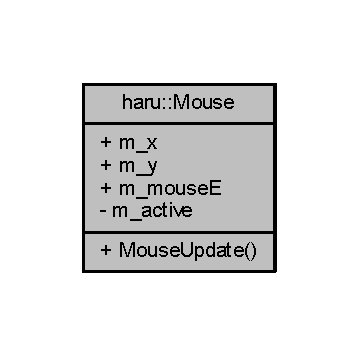
\includegraphics[width=172pt]{classharu_1_1_mouse__coll__graph}
\end{center}
\end{figure}
\subsection*{Public Member Functions}
\begin{DoxyCompactItemize}
\item 
void \mbox{\hyperlink{classharu_1_1_mouse_aa12b9821aa46840a997fdfb3e32ddd1e}{Mouse\+Update}} ()
\end{DoxyCompactItemize}
\subsection*{Public Attributes}
\begin{DoxyCompactItemize}
\item 
int \mbox{\hyperlink{classharu_1_1_mouse_a554f48ffbcb1216e483066ab8f941722}{m\+\_\+x}} = 0
\item 
int \mbox{\hyperlink{classharu_1_1_mouse_a7045facf4879e12902aeb852a894327f}{m\+\_\+y}} = 0
\item 
S\+D\+L\+\_\+\+Event \mbox{\hyperlink{classharu_1_1_mouse_ab3f417bf9a76505b33efcaff97465e71}{m\+\_\+mouseE}}
\end{DoxyCompactItemize}
\subsection*{Private Attributes}
\begin{DoxyCompactItemize}
\item 
bool \mbox{\hyperlink{classharu_1_1_mouse_a617704c4c1df5cc055a4d1f2a1414c70}{m\+\_\+active}}
\end{DoxyCompactItemize}


\subsection{Member Function Documentation}
\mbox{\Hypertarget{classharu_1_1_mouse_aa12b9821aa46840a997fdfb3e32ddd1e}\label{classharu_1_1_mouse_aa12b9821aa46840a997fdfb3e32ddd1e}} 
\index{haru\+::\+Mouse@{haru\+::\+Mouse}!Mouse\+Update@{Mouse\+Update}}
\index{Mouse\+Update@{Mouse\+Update}!haru\+::\+Mouse@{haru\+::\+Mouse}}
\subsubsection{\texorpdfstring{Mouse\+Update()}{MouseUpdate()}}
{\footnotesize\ttfamily void haru\+::\+Mouse\+::\+Mouse\+Update (\begin{DoxyParamCaption}{ }\end{DoxyParamCaption})}



\subsection{Member Data Documentation}
\mbox{\Hypertarget{classharu_1_1_mouse_a617704c4c1df5cc055a4d1f2a1414c70}\label{classharu_1_1_mouse_a617704c4c1df5cc055a4d1f2a1414c70}} 
\index{haru\+::\+Mouse@{haru\+::\+Mouse}!m\+\_\+active@{m\+\_\+active}}
\index{m\+\_\+active@{m\+\_\+active}!haru\+::\+Mouse@{haru\+::\+Mouse}}
\subsubsection{\texorpdfstring{m\+\_\+active}{m\_active}}
{\footnotesize\ttfamily bool haru\+::\+Mouse\+::m\+\_\+active\hspace{0.3cm}{\ttfamily [private]}}

\mbox{\Hypertarget{classharu_1_1_mouse_ab3f417bf9a76505b33efcaff97465e71}\label{classharu_1_1_mouse_ab3f417bf9a76505b33efcaff97465e71}} 
\index{haru\+::\+Mouse@{haru\+::\+Mouse}!m\+\_\+mouseE@{m\+\_\+mouseE}}
\index{m\+\_\+mouseE@{m\+\_\+mouseE}!haru\+::\+Mouse@{haru\+::\+Mouse}}
\subsubsection{\texorpdfstring{m\+\_\+mouseE}{m\_mouseE}}
{\footnotesize\ttfamily S\+D\+L\+\_\+\+Event haru\+::\+Mouse\+::m\+\_\+mouseE}

\mbox{\Hypertarget{classharu_1_1_mouse_a554f48ffbcb1216e483066ab8f941722}\label{classharu_1_1_mouse_a554f48ffbcb1216e483066ab8f941722}} 
\index{haru\+::\+Mouse@{haru\+::\+Mouse}!m\+\_\+x@{m\+\_\+x}}
\index{m\+\_\+x@{m\+\_\+x}!haru\+::\+Mouse@{haru\+::\+Mouse}}
\subsubsection{\texorpdfstring{m\+\_\+x}{m\_x}}
{\footnotesize\ttfamily int haru\+::\+Mouse\+::m\+\_\+x = 0}

\mbox{\Hypertarget{classharu_1_1_mouse_a7045facf4879e12902aeb852a894327f}\label{classharu_1_1_mouse_a7045facf4879e12902aeb852a894327f}} 
\index{haru\+::\+Mouse@{haru\+::\+Mouse}!m\+\_\+y@{m\+\_\+y}}
\index{m\+\_\+y@{m\+\_\+y}!haru\+::\+Mouse@{haru\+::\+Mouse}}
\subsubsection{\texorpdfstring{m\+\_\+y}{m\_y}}
{\footnotesize\ttfamily int haru\+::\+Mouse\+::m\+\_\+y = 0}



The documentation for this class was generated from the following files\+:\begin{DoxyCompactItemize}
\item 
source/haruengine/\mbox{\hyperlink{_mouse_8h}{Mouse.\+h}}\item 
source/haruengine/\mbox{\hyperlink{_mouse_8cpp}{Mouse.\+cpp}}\end{DoxyCompactItemize}

\hypertarget{classharu_1_1_object}{}\section{haru\+:\+:Object Class Reference}
\label{classharu_1_1_object}\index{haru\+::\+Object@{haru\+::\+Object}}


{\ttfamily \#include $<$Object.\+h$>$}



Collaboration diagram for haru\+:\+:Object\+:\nopagebreak
\begin{figure}[H]
\begin{center}
\leavevmode
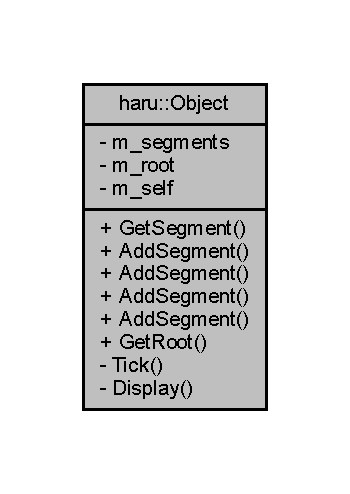
\includegraphics[width=168pt]{classharu_1_1_object__coll__graph}
\end{center}
\end{figure}
\subsection*{Public Member Functions}
\begin{DoxyCompactItemize}
\item 
{\footnotesize template$<$typename T $>$ }\\std\+::shared\+\_\+ptr$<$ T $>$ \mbox{\hyperlink{classharu_1_1_object_a7e92cffe420755e9385ddf3471a5bded}{Get\+Segment}} ()
\item 
{\footnotesize template$<$typename T $>$ }\\std\+::shared\+\_\+ptr$<$ T $>$ \mbox{\hyperlink{classharu_1_1_object_ad285384303303dd6b281a570810f18ca}{Add\+Segment}} ()
\item 
{\footnotesize template$<$typename T , typename A $>$ }\\std\+::shared\+\_\+ptr$<$ T $>$ \mbox{\hyperlink{classharu_1_1_object_a267199c40485c94b3bdc180d397a05ec}{Add\+Segment}} (A a)
\item 
{\footnotesize template$<$typename T , typename A , typename B $>$ }\\std\+::shared\+\_\+ptr$<$ T $>$ \mbox{\hyperlink{classharu_1_1_object_a31a365466f2ea7b3a0b41d1942f29f59}{Add\+Segment}} (A a, B b)
\item 
{\footnotesize template$<$typename T , typename A , typename B , typename C $>$ }\\std\+::shared\+\_\+ptr$<$ T $>$ \mbox{\hyperlink{classharu_1_1_object_afa6249bdd2fe914f724289884ddd5a51}{Add\+Segment}} (A a, B b, C c)
\item 
std\+::shared\+\_\+ptr$<$ \mbox{\hyperlink{classharu_1_1_root}{Root}} $>$ \mbox{\hyperlink{classharu_1_1_object_a4c4a67d8ba840d295876f80a12163281}{Get\+Root}} ()
\end{DoxyCompactItemize}
\subsection*{Private Member Functions}
\begin{DoxyCompactItemize}
\item 
void \mbox{\hyperlink{classharu_1_1_object_a38daa375a6573f00fa150848fc3a6dde}{Tick}} ()
\item 
void \mbox{\hyperlink{classharu_1_1_object_a18e746943f998314aa27ffb96dac71cb}{Display}} ()
\end{DoxyCompactItemize}
\subsection*{Private Attributes}
\begin{DoxyCompactItemize}
\item 
std\+::vector$<$ std\+::shared\+\_\+ptr$<$ \mbox{\hyperlink{classharu_1_1_segment}{Segment}} $>$ $>$ \mbox{\hyperlink{classharu_1_1_object_a657dae7e9caa350f40aac59d5c734ad1}{m\+\_\+segments}}
\item 
std\+::weak\+\_\+ptr$<$ \mbox{\hyperlink{classharu_1_1_root}{Root}} $>$ \mbox{\hyperlink{classharu_1_1_object_a46facc31fd20aa99a248e4bdb063a043}{m\+\_\+root}}
\item 
std\+::weak\+\_\+ptr$<$ \mbox{\hyperlink{classharu_1_1_object}{Object}} $>$ \mbox{\hyperlink{classharu_1_1_object_ae204b014fc8c7bedc74508da20420769}{m\+\_\+self}}
\end{DoxyCompactItemize}
\subsection*{Friends}
\begin{DoxyCompactItemize}
\item 
class \mbox{\hyperlink{classharu_1_1_object_a4966338964dbcd90cba2a6b4bd1b3521}{Root}}
\end{DoxyCompactItemize}


\subsection{Member Function Documentation}
\mbox{\Hypertarget{classharu_1_1_object_ad285384303303dd6b281a570810f18ca}\label{classharu_1_1_object_ad285384303303dd6b281a570810f18ca}} 
\index{haru\+::\+Object@{haru\+::\+Object}!Add\+Segment@{Add\+Segment}}
\index{Add\+Segment@{Add\+Segment}!haru\+::\+Object@{haru\+::\+Object}}
\subsubsection{\texorpdfstring{Add\+Segment()}{AddSegment()}\hspace{0.1cm}{\footnotesize\ttfamily [1/4]}}
{\footnotesize\ttfamily template$<$typename T $>$ \\
std\+::shared\+\_\+ptr$<$T$>$ haru\+::\+Object\+::\+Add\+Segment (\begin{DoxyParamCaption}{ }\end{DoxyParamCaption})\hspace{0.3cm}{\ttfamily [inline]}}

\mbox{\Hypertarget{classharu_1_1_object_a267199c40485c94b3bdc180d397a05ec}\label{classharu_1_1_object_a267199c40485c94b3bdc180d397a05ec}} 
\index{haru\+::\+Object@{haru\+::\+Object}!Add\+Segment@{Add\+Segment}}
\index{Add\+Segment@{Add\+Segment}!haru\+::\+Object@{haru\+::\+Object}}
\subsubsection{\texorpdfstring{Add\+Segment()}{AddSegment()}\hspace{0.1cm}{\footnotesize\ttfamily [2/4]}}
{\footnotesize\ttfamily template$<$typename T , typename A $>$ \\
std\+::shared\+\_\+ptr$<$T$>$ haru\+::\+Object\+::\+Add\+Segment (\begin{DoxyParamCaption}\item[{A}]{a }\end{DoxyParamCaption})\hspace{0.3cm}{\ttfamily [inline]}}

\mbox{\Hypertarget{classharu_1_1_object_a31a365466f2ea7b3a0b41d1942f29f59}\label{classharu_1_1_object_a31a365466f2ea7b3a0b41d1942f29f59}} 
\index{haru\+::\+Object@{haru\+::\+Object}!Add\+Segment@{Add\+Segment}}
\index{Add\+Segment@{Add\+Segment}!haru\+::\+Object@{haru\+::\+Object}}
\subsubsection{\texorpdfstring{Add\+Segment()}{AddSegment()}\hspace{0.1cm}{\footnotesize\ttfamily [3/4]}}
{\footnotesize\ttfamily template$<$typename T , typename A , typename B $>$ \\
std\+::shared\+\_\+ptr$<$T$>$ haru\+::\+Object\+::\+Add\+Segment (\begin{DoxyParamCaption}\item[{A}]{a,  }\item[{B}]{b }\end{DoxyParamCaption})\hspace{0.3cm}{\ttfamily [inline]}}

\mbox{\Hypertarget{classharu_1_1_object_afa6249bdd2fe914f724289884ddd5a51}\label{classharu_1_1_object_afa6249bdd2fe914f724289884ddd5a51}} 
\index{haru\+::\+Object@{haru\+::\+Object}!Add\+Segment@{Add\+Segment}}
\index{Add\+Segment@{Add\+Segment}!haru\+::\+Object@{haru\+::\+Object}}
\subsubsection{\texorpdfstring{Add\+Segment()}{AddSegment()}\hspace{0.1cm}{\footnotesize\ttfamily [4/4]}}
{\footnotesize\ttfamily template$<$typename T , typename A , typename B , typename C $>$ \\
std\+::shared\+\_\+ptr$<$T$>$ haru\+::\+Object\+::\+Add\+Segment (\begin{DoxyParamCaption}\item[{A}]{a,  }\item[{B}]{b,  }\item[{C}]{c }\end{DoxyParamCaption})\hspace{0.3cm}{\ttfamily [inline]}}

\mbox{\Hypertarget{classharu_1_1_object_a18e746943f998314aa27ffb96dac71cb}\label{classharu_1_1_object_a18e746943f998314aa27ffb96dac71cb}} 
\index{haru\+::\+Object@{haru\+::\+Object}!Display@{Display}}
\index{Display@{Display}!haru\+::\+Object@{haru\+::\+Object}}
\subsubsection{\texorpdfstring{Display()}{Display()}}
{\footnotesize\ttfamily void haru\+::\+Object\+::\+Display (\begin{DoxyParamCaption}{ }\end{DoxyParamCaption})\hspace{0.3cm}{\ttfamily [private]}}

\mbox{\Hypertarget{classharu_1_1_object_a4c4a67d8ba840d295876f80a12163281}\label{classharu_1_1_object_a4c4a67d8ba840d295876f80a12163281}} 
\index{haru\+::\+Object@{haru\+::\+Object}!Get\+Root@{Get\+Root}}
\index{Get\+Root@{Get\+Root}!haru\+::\+Object@{haru\+::\+Object}}
\subsubsection{\texorpdfstring{Get\+Root()}{GetRoot()}}
{\footnotesize\ttfamily std\+::shared\+\_\+ptr$<$ \mbox{\hyperlink{classharu_1_1_root}{Root}} $>$ haru\+::\+Object\+::\+Get\+Root (\begin{DoxyParamCaption}{ }\end{DoxyParamCaption})}

\mbox{\Hypertarget{classharu_1_1_object_a7e92cffe420755e9385ddf3471a5bded}\label{classharu_1_1_object_a7e92cffe420755e9385ddf3471a5bded}} 
\index{haru\+::\+Object@{haru\+::\+Object}!Get\+Segment@{Get\+Segment}}
\index{Get\+Segment@{Get\+Segment}!haru\+::\+Object@{haru\+::\+Object}}
\subsubsection{\texorpdfstring{Get\+Segment()}{GetSegment()}}
{\footnotesize\ttfamily template$<$typename T $>$ \\
std\+::shared\+\_\+ptr$<$T$>$ haru\+::\+Object\+::\+Get\+Segment (\begin{DoxyParamCaption}{ }\end{DoxyParamCaption})\hspace{0.3cm}{\ttfamily [inline]}}

\mbox{\Hypertarget{classharu_1_1_object_a38daa375a6573f00fa150848fc3a6dde}\label{classharu_1_1_object_a38daa375a6573f00fa150848fc3a6dde}} 
\index{haru\+::\+Object@{haru\+::\+Object}!Tick@{Tick}}
\index{Tick@{Tick}!haru\+::\+Object@{haru\+::\+Object}}
\subsubsection{\texorpdfstring{Tick()}{Tick()}}
{\footnotesize\ttfamily void haru\+::\+Object\+::\+Tick (\begin{DoxyParamCaption}{ }\end{DoxyParamCaption})\hspace{0.3cm}{\ttfamily [private]}}



\subsection{Friends And Related Function Documentation}
\mbox{\Hypertarget{classharu_1_1_object_a4966338964dbcd90cba2a6b4bd1b3521}\label{classharu_1_1_object_a4966338964dbcd90cba2a6b4bd1b3521}} 
\index{haru\+::\+Object@{haru\+::\+Object}!Root@{Root}}
\index{Root@{Root}!haru\+::\+Object@{haru\+::\+Object}}
\subsubsection{\texorpdfstring{Root}{Root}}
{\footnotesize\ttfamily friend class \mbox{\hyperlink{classharu_1_1_root}{Root}}\hspace{0.3cm}{\ttfamily [friend]}}



\subsection{Member Data Documentation}
\mbox{\Hypertarget{classharu_1_1_object_a46facc31fd20aa99a248e4bdb063a043}\label{classharu_1_1_object_a46facc31fd20aa99a248e4bdb063a043}} 
\index{haru\+::\+Object@{haru\+::\+Object}!m\+\_\+root@{m\+\_\+root}}
\index{m\+\_\+root@{m\+\_\+root}!haru\+::\+Object@{haru\+::\+Object}}
\subsubsection{\texorpdfstring{m\+\_\+root}{m\_root}}
{\footnotesize\ttfamily std\+::weak\+\_\+ptr$<$\mbox{\hyperlink{classharu_1_1_root}{Root}}$>$ haru\+::\+Object\+::m\+\_\+root\hspace{0.3cm}{\ttfamily [private]}}

\mbox{\Hypertarget{classharu_1_1_object_a657dae7e9caa350f40aac59d5c734ad1}\label{classharu_1_1_object_a657dae7e9caa350f40aac59d5c734ad1}} 
\index{haru\+::\+Object@{haru\+::\+Object}!m\+\_\+segments@{m\+\_\+segments}}
\index{m\+\_\+segments@{m\+\_\+segments}!haru\+::\+Object@{haru\+::\+Object}}
\subsubsection{\texorpdfstring{m\+\_\+segments}{m\_segments}}
{\footnotesize\ttfamily std\+::vector$<$std\+::shared\+\_\+ptr$<$\mbox{\hyperlink{classharu_1_1_segment}{Segment}}$>$ $>$ haru\+::\+Object\+::m\+\_\+segments\hspace{0.3cm}{\ttfamily [private]}}

\mbox{\Hypertarget{classharu_1_1_object_ae204b014fc8c7bedc74508da20420769}\label{classharu_1_1_object_ae204b014fc8c7bedc74508da20420769}} 
\index{haru\+::\+Object@{haru\+::\+Object}!m\+\_\+self@{m\+\_\+self}}
\index{m\+\_\+self@{m\+\_\+self}!haru\+::\+Object@{haru\+::\+Object}}
\subsubsection{\texorpdfstring{m\+\_\+self}{m\_self}}
{\footnotesize\ttfamily std\+::weak\+\_\+ptr$<$\mbox{\hyperlink{classharu_1_1_object}{Object}}$>$ haru\+::\+Object\+::m\+\_\+self\hspace{0.3cm}{\ttfamily [private]}}



The documentation for this class was generated from the following files\+:\begin{DoxyCompactItemize}
\item 
source/haruengine/\mbox{\hyperlink{_object_8h}{Object.\+h}}\item 
source/haruengine/\mbox{\hyperlink{_object_8cpp}{Object.\+cpp}}\end{DoxyCompactItemize}

\hypertarget{structharu_1_1_re_mesh}{}\section{haru\+:\+:Re\+Mesh Struct Reference}
\label{structharu_1_1_re_mesh}\index{haru\+::\+Re\+Mesh@{haru\+::\+Re\+Mesh}}


{\ttfamily \#include $<$Resource.\+h$>$}



Collaboration diagram for haru\+:\+:Re\+Mesh\+:\nopagebreak
\begin{figure}[H]
\begin{center}
\leavevmode
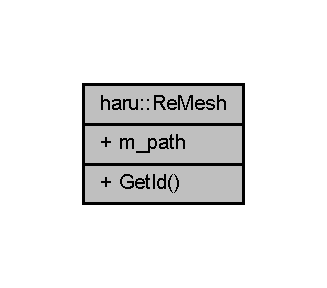
\includegraphics[width=157pt]{structharu_1_1_re_mesh__coll__graph}
\end{center}
\end{figure}
\subsection*{Public Member Functions}
\begin{DoxyCompactItemize}
\item 
G\+Luint \mbox{\hyperlink{structharu_1_1_re_mesh_a6be6fd0e97e1e9754baa68eef4383923}{Get\+Id}} ()
\end{DoxyCompactItemize}
\subsection*{Public Attributes}
\begin{DoxyCompactItemize}
\item 
std\+::string \mbox{\hyperlink{structharu_1_1_re_mesh_ae4a023863733f58bd9dabfde91f30f05}{m\+\_\+path}}
\end{DoxyCompactItemize}


\subsection{Member Function Documentation}
\mbox{\Hypertarget{structharu_1_1_re_mesh_a6be6fd0e97e1e9754baa68eef4383923}\label{structharu_1_1_re_mesh_a6be6fd0e97e1e9754baa68eef4383923}} 
\index{haru\+::\+Re\+Mesh@{haru\+::\+Re\+Mesh}!Get\+Id@{Get\+Id}}
\index{Get\+Id@{Get\+Id}!haru\+::\+Re\+Mesh@{haru\+::\+Re\+Mesh}}
\subsubsection{\texorpdfstring{Get\+Id()}{GetId()}}
{\footnotesize\ttfamily G\+Luint haru\+::\+Re\+Mesh\+::\+Get\+Id (\begin{DoxyParamCaption}{ }\end{DoxyParamCaption})}



\subsection{Member Data Documentation}
\mbox{\Hypertarget{structharu_1_1_re_mesh_ae4a023863733f58bd9dabfde91f30f05}\label{structharu_1_1_re_mesh_ae4a023863733f58bd9dabfde91f30f05}} 
\index{haru\+::\+Re\+Mesh@{haru\+::\+Re\+Mesh}!m\+\_\+path@{m\+\_\+path}}
\index{m\+\_\+path@{m\+\_\+path}!haru\+::\+Re\+Mesh@{haru\+::\+Re\+Mesh}}
\subsubsection{\texorpdfstring{m\+\_\+path}{m\_path}}
{\footnotesize\ttfamily std\+::string haru\+::\+Re\+Mesh\+::m\+\_\+path}



The documentation for this struct was generated from the following file\+:\begin{DoxyCompactItemize}
\item 
source/haruengine/\mbox{\hyperlink{_resource_8h}{Resource.\+h}}\end{DoxyCompactItemize}

\hypertarget{classharu_1_1_render_texture}{}\section{haru\+:\+:Render\+Texture Class Reference}
\label{classharu_1_1_render_texture}\index{haru\+::\+Render\+Texture@{haru\+::\+Render\+Texture}}


{\ttfamily \#include $<$Render\+Texture.\+h$>$}



Inheritance diagram for haru\+:\+:Render\+Texture\+:\nopagebreak
\begin{figure}[H]
\begin{center}
\leavevmode
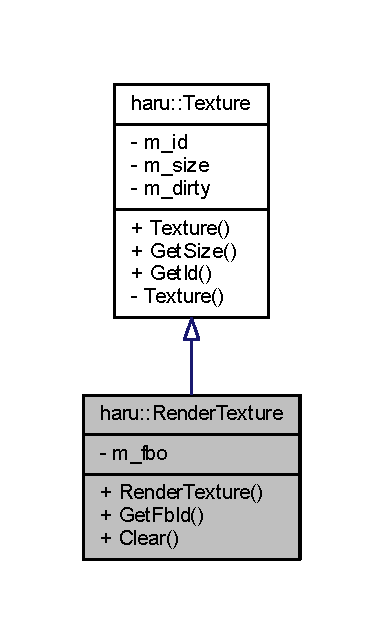
\includegraphics[width=184pt]{classharu_1_1_render_texture__inherit__graph}
\end{center}
\end{figure}


Collaboration diagram for haru\+:\+:Render\+Texture\+:\nopagebreak
\begin{figure}[H]
\begin{center}
\leavevmode
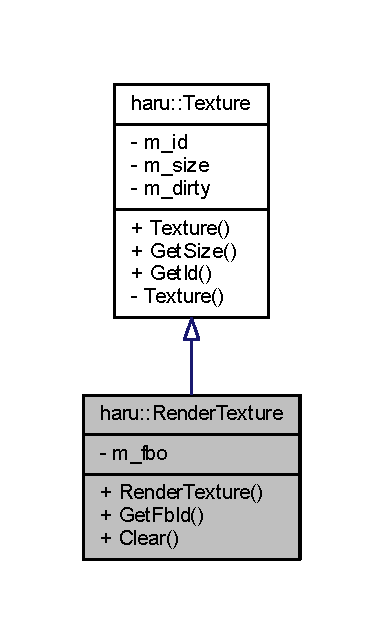
\includegraphics[width=184pt]{classharu_1_1_render_texture__coll__graph}
\end{center}
\end{figure}
\subsection*{Public Member Functions}
\begin{DoxyCompactItemize}
\item 
\mbox{\hyperlink{classharu_1_1_render_texture_a4b28ec612c35cbfa80f3205511351e7a}{Render\+Texture}} (int \+\_\+width, int \+\_\+height)
\item 
G\+Luint \mbox{\hyperlink{classharu_1_1_render_texture_acafa41032f3c155504d130c5ae43600b}{Get\+Fb\+Id}} ()
\item 
void \mbox{\hyperlink{classharu_1_1_render_texture_a923dfcb8a68d98c258de7f795a822721}{Clear}} ()
\end{DoxyCompactItemize}
\subsection*{Private Attributes}
\begin{DoxyCompactItemize}
\item 
G\+Luint \mbox{\hyperlink{classharu_1_1_render_texture_aa41c747cc61bf1c34fa64422cfdacc8c}{m\+\_\+fbo}}
\end{DoxyCompactItemize}


\subsection{Constructor \& Destructor Documentation}
\mbox{\Hypertarget{classharu_1_1_render_texture_a4b28ec612c35cbfa80f3205511351e7a}\label{classharu_1_1_render_texture_a4b28ec612c35cbfa80f3205511351e7a}} 
\index{haru\+::\+Render\+Texture@{haru\+::\+Render\+Texture}!Render\+Texture@{Render\+Texture}}
\index{Render\+Texture@{Render\+Texture}!haru\+::\+Render\+Texture@{haru\+::\+Render\+Texture}}
\subsubsection{\texorpdfstring{Render\+Texture()}{RenderTexture()}}
{\footnotesize\ttfamily haru\+::\+Render\+Texture\+::\+Render\+Texture (\begin{DoxyParamCaption}\item[{int}]{\+\_\+width,  }\item[{int}]{\+\_\+height }\end{DoxyParamCaption})}



\subsection{Member Function Documentation}
\mbox{\Hypertarget{classharu_1_1_render_texture_a923dfcb8a68d98c258de7f795a822721}\label{classharu_1_1_render_texture_a923dfcb8a68d98c258de7f795a822721}} 
\index{haru\+::\+Render\+Texture@{haru\+::\+Render\+Texture}!Clear@{Clear}}
\index{Clear@{Clear}!haru\+::\+Render\+Texture@{haru\+::\+Render\+Texture}}
\subsubsection{\texorpdfstring{Clear()}{Clear()}}
{\footnotesize\ttfamily void haru\+::\+Render\+Texture\+::\+Clear (\begin{DoxyParamCaption}{ }\end{DoxyParamCaption})}

\mbox{\Hypertarget{classharu_1_1_render_texture_acafa41032f3c155504d130c5ae43600b}\label{classharu_1_1_render_texture_acafa41032f3c155504d130c5ae43600b}} 
\index{haru\+::\+Render\+Texture@{haru\+::\+Render\+Texture}!Get\+Fb\+Id@{Get\+Fb\+Id}}
\index{Get\+Fb\+Id@{Get\+Fb\+Id}!haru\+::\+Render\+Texture@{haru\+::\+Render\+Texture}}
\subsubsection{\texorpdfstring{Get\+Fb\+Id()}{GetFbId()}}
{\footnotesize\ttfamily G\+Luint haru\+::\+Render\+Texture\+::\+Get\+Fb\+Id (\begin{DoxyParamCaption}{ }\end{DoxyParamCaption})}



\subsection{Member Data Documentation}
\mbox{\Hypertarget{classharu_1_1_render_texture_aa41c747cc61bf1c34fa64422cfdacc8c}\label{classharu_1_1_render_texture_aa41c747cc61bf1c34fa64422cfdacc8c}} 
\index{haru\+::\+Render\+Texture@{haru\+::\+Render\+Texture}!m\+\_\+fbo@{m\+\_\+fbo}}
\index{m\+\_\+fbo@{m\+\_\+fbo}!haru\+::\+Render\+Texture@{haru\+::\+Render\+Texture}}
\subsubsection{\texorpdfstring{m\+\_\+fbo}{m\_fbo}}
{\footnotesize\ttfamily G\+Luint haru\+::\+Render\+Texture\+::m\+\_\+fbo\hspace{0.3cm}{\ttfamily [private]}}



The documentation for this class was generated from the following files\+:\begin{DoxyCompactItemize}
\item 
source/haruengine/\mbox{\hyperlink{_render_texture_8h}{Render\+Texture.\+h}}\item 
source/haruengine/\mbox{\hyperlink{_render_texture_8cpp}{Render\+Texture.\+cpp}}\end{DoxyCompactItemize}

\hypertarget{classharu_1_1_resource}{}\section{haru\+:\+:Resource Class Reference}
\label{classharu_1_1_resource}\index{haru\+::\+Resource@{haru\+::\+Resource}}


{\ttfamily \#include $<$Resource.\+h$>$}



Collaboration diagram for haru\+:\+:Resource\+:\nopagebreak
\begin{figure}[H]
\begin{center}
\leavevmode
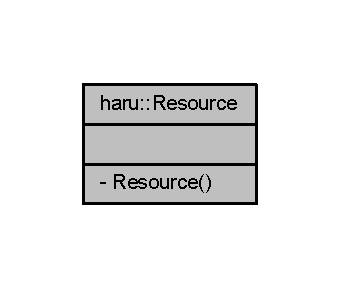
\includegraphics[width=163pt]{classharu_1_1_resource__coll__graph}
\end{center}
\end{figure}
\subsection*{Private Member Functions}
\begin{DoxyCompactItemize}
\item 
\mbox{\hyperlink{classharu_1_1_resource_a338ffdb66c7c406e5bc59870c4154550}{Resource}} ()
\end{DoxyCompactItemize}


\subsection{Constructor \& Destructor Documentation}
\mbox{\Hypertarget{classharu_1_1_resource_a338ffdb66c7c406e5bc59870c4154550}\label{classharu_1_1_resource_a338ffdb66c7c406e5bc59870c4154550}} 
\index{haru\+::\+Resource@{haru\+::\+Resource}!Resource@{Resource}}
\index{Resource@{Resource}!haru\+::\+Resource@{haru\+::\+Resource}}
\subsubsection{\texorpdfstring{Resource()}{Resource()}}
{\footnotesize\ttfamily haru\+::\+Resource\+::\+Resource (\begin{DoxyParamCaption}{ }\end{DoxyParamCaption})\hspace{0.3cm}{\ttfamily [private]}}



The documentation for this class was generated from the following file\+:\begin{DoxyCompactItemize}
\item 
source/haruengine/\mbox{\hyperlink{_resource_8h}{Resource.\+h}}\end{DoxyCompactItemize}

\hypertarget{classharu_1_1_root}{}\section{haru\+:\+:Root Class Reference}
\label{classharu_1_1_root}\index{haru\+::\+Root@{haru\+::\+Root}}


{\ttfamily \#include $<$Root.\+h$>$}



Collaboration diagram for haru\+:\+:Root\+:\nopagebreak
\begin{figure}[H]
\begin{center}
\leavevmode
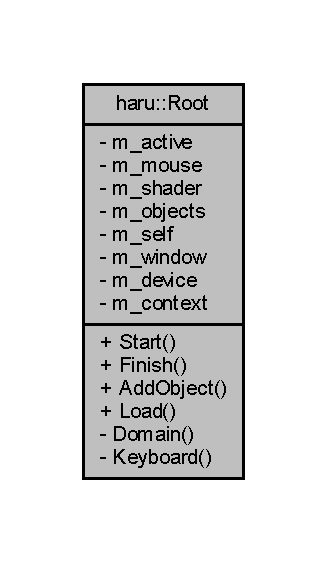
\includegraphics[width=157pt]{classharu_1_1_root__coll__graph}
\end{center}
\end{figure}
\subsection*{Public Member Functions}
\begin{DoxyCompactItemize}
\item 
void \mbox{\hyperlink{classharu_1_1_root_aedc20d4891295ccb1129a5b386a7906b}{Start}} ()
\item 
void \mbox{\hyperlink{classharu_1_1_root_aa0767148d14c4c9bc06bf41d3a44188f}{Finish}} ()
\item 
std\+::shared\+\_\+ptr$<$ \mbox{\hyperlink{classharu_1_1_object}{Object}} $>$ \mbox{\hyperlink{classharu_1_1_root_a058a9ead82bdc50ef1f8e08413c72131}{Add\+Object}} ()
\end{DoxyCompactItemize}
\subsection*{Static Public Member Functions}
\begin{DoxyCompactItemize}
\item 
static std\+::shared\+\_\+ptr$<$ \mbox{\hyperlink{classharu_1_1_root}{Root}} $>$ \mbox{\hyperlink{classharu_1_1_root_a99a344889111b264e42a1ad724a5ceae}{Load}} ()
\end{DoxyCompactItemize}
\subsection*{Private Member Functions}
\begin{DoxyCompactItemize}
\item 
std\+::shared\+\_\+ptr$<$ \mbox{\hyperlink{class_domain}{Domain}} $>$ \mbox{\hyperlink{classharu_1_1_root_a1fd00f081aeeaf09eea1347bdd22ba2a}{Domain}} ()
\item 
std\+::shared\+\_\+ptr$<$ \mbox{\hyperlink{class_keyboard}{Keyboard}} $>$ \mbox{\hyperlink{classharu_1_1_root_a4d3ca0f98e581f98868f76e003c6d710}{Keyboard}} ()
\end{DoxyCompactItemize}
\subsection*{Private Attributes}
\begin{DoxyCompactItemize}
\item 
bool \mbox{\hyperlink{classharu_1_1_root_a5e251a25155fd4cb55b488b6520e1bd4}{m\+\_\+active}}
\item 
std\+::shared\+\_\+ptr$<$ \mbox{\hyperlink{classharu_1_1_mouse}{Mouse}} $>$ \mbox{\hyperlink{classharu_1_1_root_a1d9f5606aebb0fda4a6eb5ca5970c9d1}{m\+\_\+mouse}}
\item 
std\+::shared\+\_\+ptr$<$ \mbox{\hyperlink{classharu_1_1_shader_program}{Shader\+Program}} $>$ \mbox{\hyperlink{classharu_1_1_root_af62f9d3dc17742091234295bd4c6bac4}{m\+\_\+shader}}
\item 
std\+::vector$<$ std\+::shared\+\_\+ptr$<$ \mbox{\hyperlink{classharu_1_1_object}{Object}} $>$ $>$ \mbox{\hyperlink{classharu_1_1_root_a1c2da39d062cc0ccaba26ba446baaa88}{m\+\_\+objects}}
\item 
std\+::weak\+\_\+ptr$<$ \mbox{\hyperlink{classharu_1_1_root}{Root}} $>$ \mbox{\hyperlink{classharu_1_1_root_a36ccda976146da69253d0de01641dbec}{m\+\_\+self}}
\item 
S\+D\+L\+\_\+\+Window $\ast$ \mbox{\hyperlink{classharu_1_1_root_a91725127201f71d5a1f2aebfafac499c}{m\+\_\+window}}
\item 
A\+L\+Cdevice $\ast$ \mbox{\hyperlink{classharu_1_1_root_afaeed3289f7697f80c3b71a68c98db2f}{m\+\_\+device}}
\item 
A\+L\+Ccontext $\ast$ \mbox{\hyperlink{classharu_1_1_root_a922896e42c7813ef55bff4011d12ab88}{m\+\_\+context}}
\end{DoxyCompactItemize}


\subsection{Member Function Documentation}
\mbox{\Hypertarget{classharu_1_1_root_a058a9ead82bdc50ef1f8e08413c72131}\label{classharu_1_1_root_a058a9ead82bdc50ef1f8e08413c72131}} 
\index{haru\+::\+Root@{haru\+::\+Root}!Add\+Object@{Add\+Object}}
\index{Add\+Object@{Add\+Object}!haru\+::\+Root@{haru\+::\+Root}}
\subsubsection{\texorpdfstring{Add\+Object()}{AddObject()}}
{\footnotesize\ttfamily std\+::shared\+\_\+ptr$<$ \mbox{\hyperlink{classharu_1_1_object}{Object}} $>$ haru\+::\+Root\+::\+Add\+Object (\begin{DoxyParamCaption}{ }\end{DoxyParamCaption})}

\mbox{\Hypertarget{classharu_1_1_root_a1fd00f081aeeaf09eea1347bdd22ba2a}\label{classharu_1_1_root_a1fd00f081aeeaf09eea1347bdd22ba2a}} 
\index{haru\+::\+Root@{haru\+::\+Root}!Domain@{Domain}}
\index{Domain@{Domain}!haru\+::\+Root@{haru\+::\+Root}}
\subsubsection{\texorpdfstring{Domain()}{Domain()}}
{\footnotesize\ttfamily std\+::shared\+\_\+ptr$<$ \mbox{\hyperlink{class_domain}{Domain}} $>$ haru\+::\+Root\+::\+Domain (\begin{DoxyParamCaption}{ }\end{DoxyParamCaption})\hspace{0.3cm}{\ttfamily [private]}}

\mbox{\Hypertarget{classharu_1_1_root_aa0767148d14c4c9bc06bf41d3a44188f}\label{classharu_1_1_root_aa0767148d14c4c9bc06bf41d3a44188f}} 
\index{haru\+::\+Root@{haru\+::\+Root}!Finish@{Finish}}
\index{Finish@{Finish}!haru\+::\+Root@{haru\+::\+Root}}
\subsubsection{\texorpdfstring{Finish()}{Finish()}}
{\footnotesize\ttfamily void haru\+::\+Root\+::\+Finish (\begin{DoxyParamCaption}{ }\end{DoxyParamCaption})}

\mbox{\Hypertarget{classharu_1_1_root_a4d3ca0f98e581f98868f76e003c6d710}\label{classharu_1_1_root_a4d3ca0f98e581f98868f76e003c6d710}} 
\index{haru\+::\+Root@{haru\+::\+Root}!Keyboard@{Keyboard}}
\index{Keyboard@{Keyboard}!haru\+::\+Root@{haru\+::\+Root}}
\subsubsection{\texorpdfstring{Keyboard()}{Keyboard()}}
{\footnotesize\ttfamily std\+::shared\+\_\+ptr$<$ \mbox{\hyperlink{class_keyboard}{Keyboard}} $>$ haru\+::\+Root\+::\+Keyboard (\begin{DoxyParamCaption}{ }\end{DoxyParamCaption})\hspace{0.3cm}{\ttfamily [private]}}

\mbox{\Hypertarget{classharu_1_1_root_a99a344889111b264e42a1ad724a5ceae}\label{classharu_1_1_root_a99a344889111b264e42a1ad724a5ceae}} 
\index{haru\+::\+Root@{haru\+::\+Root}!Load@{Load}}
\index{Load@{Load}!haru\+::\+Root@{haru\+::\+Root}}
\subsubsection{\texorpdfstring{Load()}{Load()}}
{\footnotesize\ttfamily std\+::shared\+\_\+ptr$<$ \mbox{\hyperlink{classharu_1_1_root}{Root}} $>$ haru\+::\+Root\+::\+Load (\begin{DoxyParamCaption}{ }\end{DoxyParamCaption})\hspace{0.3cm}{\ttfamily [static]}}

Here is the caller graph for this function\+:
\nopagebreak
\begin{figure}[H]
\begin{center}
\leavevmode
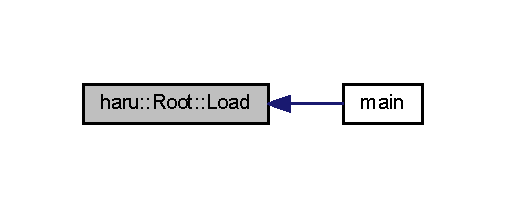
\includegraphics[width=243pt]{classharu_1_1_root_a99a344889111b264e42a1ad724a5ceae_icgraph}
\end{center}
\end{figure}
\mbox{\Hypertarget{classharu_1_1_root_aedc20d4891295ccb1129a5b386a7906b}\label{classharu_1_1_root_aedc20d4891295ccb1129a5b386a7906b}} 
\index{haru\+::\+Root@{haru\+::\+Root}!Start@{Start}}
\index{Start@{Start}!haru\+::\+Root@{haru\+::\+Root}}
\subsubsection{\texorpdfstring{Start()}{Start()}}
{\footnotesize\ttfamily void haru\+::\+Root\+::\+Start (\begin{DoxyParamCaption}{ }\end{DoxyParamCaption})}



\subsection{Member Data Documentation}
\mbox{\Hypertarget{classharu_1_1_root_a5e251a25155fd4cb55b488b6520e1bd4}\label{classharu_1_1_root_a5e251a25155fd4cb55b488b6520e1bd4}} 
\index{haru\+::\+Root@{haru\+::\+Root}!m\+\_\+active@{m\+\_\+active}}
\index{m\+\_\+active@{m\+\_\+active}!haru\+::\+Root@{haru\+::\+Root}}
\subsubsection{\texorpdfstring{m\+\_\+active}{m\_active}}
{\footnotesize\ttfamily bool haru\+::\+Root\+::m\+\_\+active\hspace{0.3cm}{\ttfamily [private]}}

\mbox{\Hypertarget{classharu_1_1_root_a922896e42c7813ef55bff4011d12ab88}\label{classharu_1_1_root_a922896e42c7813ef55bff4011d12ab88}} 
\index{haru\+::\+Root@{haru\+::\+Root}!m\+\_\+context@{m\+\_\+context}}
\index{m\+\_\+context@{m\+\_\+context}!haru\+::\+Root@{haru\+::\+Root}}
\subsubsection{\texorpdfstring{m\+\_\+context}{m\_context}}
{\footnotesize\ttfamily A\+L\+Ccontext$\ast$ haru\+::\+Root\+::m\+\_\+context\hspace{0.3cm}{\ttfamily [private]}}

\mbox{\Hypertarget{classharu_1_1_root_afaeed3289f7697f80c3b71a68c98db2f}\label{classharu_1_1_root_afaeed3289f7697f80c3b71a68c98db2f}} 
\index{haru\+::\+Root@{haru\+::\+Root}!m\+\_\+device@{m\+\_\+device}}
\index{m\+\_\+device@{m\+\_\+device}!haru\+::\+Root@{haru\+::\+Root}}
\subsubsection{\texorpdfstring{m\+\_\+device}{m\_device}}
{\footnotesize\ttfamily A\+L\+Cdevice$\ast$ haru\+::\+Root\+::m\+\_\+device\hspace{0.3cm}{\ttfamily [private]}}

\mbox{\Hypertarget{classharu_1_1_root_a1d9f5606aebb0fda4a6eb5ca5970c9d1}\label{classharu_1_1_root_a1d9f5606aebb0fda4a6eb5ca5970c9d1}} 
\index{haru\+::\+Root@{haru\+::\+Root}!m\+\_\+mouse@{m\+\_\+mouse}}
\index{m\+\_\+mouse@{m\+\_\+mouse}!haru\+::\+Root@{haru\+::\+Root}}
\subsubsection{\texorpdfstring{m\+\_\+mouse}{m\_mouse}}
{\footnotesize\ttfamily std\+::shared\+\_\+ptr$<$\mbox{\hyperlink{classharu_1_1_mouse}{Mouse}}$>$ haru\+::\+Root\+::m\+\_\+mouse\hspace{0.3cm}{\ttfamily [private]}}

\mbox{\Hypertarget{classharu_1_1_root_a1c2da39d062cc0ccaba26ba446baaa88}\label{classharu_1_1_root_a1c2da39d062cc0ccaba26ba446baaa88}} 
\index{haru\+::\+Root@{haru\+::\+Root}!m\+\_\+objects@{m\+\_\+objects}}
\index{m\+\_\+objects@{m\+\_\+objects}!haru\+::\+Root@{haru\+::\+Root}}
\subsubsection{\texorpdfstring{m\+\_\+objects}{m\_objects}}
{\footnotesize\ttfamily std\+::vector$<$std\+::shared\+\_\+ptr$<$\mbox{\hyperlink{classharu_1_1_object}{Object}}$>$ $>$ haru\+::\+Root\+::m\+\_\+objects\hspace{0.3cm}{\ttfamily [private]}}

\mbox{\Hypertarget{classharu_1_1_root_a36ccda976146da69253d0de01641dbec}\label{classharu_1_1_root_a36ccda976146da69253d0de01641dbec}} 
\index{haru\+::\+Root@{haru\+::\+Root}!m\+\_\+self@{m\+\_\+self}}
\index{m\+\_\+self@{m\+\_\+self}!haru\+::\+Root@{haru\+::\+Root}}
\subsubsection{\texorpdfstring{m\+\_\+self}{m\_self}}
{\footnotesize\ttfamily std\+::weak\+\_\+ptr$<$\mbox{\hyperlink{classharu_1_1_root}{Root}}$>$ haru\+::\+Root\+::m\+\_\+self\hspace{0.3cm}{\ttfamily [private]}}

\mbox{\Hypertarget{classharu_1_1_root_af62f9d3dc17742091234295bd4c6bac4}\label{classharu_1_1_root_af62f9d3dc17742091234295bd4c6bac4}} 
\index{haru\+::\+Root@{haru\+::\+Root}!m\+\_\+shader@{m\+\_\+shader}}
\index{m\+\_\+shader@{m\+\_\+shader}!haru\+::\+Root@{haru\+::\+Root}}
\subsubsection{\texorpdfstring{m\+\_\+shader}{m\_shader}}
{\footnotesize\ttfamily std\+::shared\+\_\+ptr$<$\mbox{\hyperlink{classharu_1_1_shader_program}{Shader\+Program}}$>$ haru\+::\+Root\+::m\+\_\+shader\hspace{0.3cm}{\ttfamily [private]}}

\mbox{\Hypertarget{classharu_1_1_root_a91725127201f71d5a1f2aebfafac499c}\label{classharu_1_1_root_a91725127201f71d5a1f2aebfafac499c}} 
\index{haru\+::\+Root@{haru\+::\+Root}!m\+\_\+window@{m\+\_\+window}}
\index{m\+\_\+window@{m\+\_\+window}!haru\+::\+Root@{haru\+::\+Root}}
\subsubsection{\texorpdfstring{m\+\_\+window}{m\_window}}
{\footnotesize\ttfamily S\+D\+L\+\_\+\+Window$\ast$ haru\+::\+Root\+::m\+\_\+window\hspace{0.3cm}{\ttfamily [private]}}



The documentation for this class was generated from the following files\+:\begin{DoxyCompactItemize}
\item 
source/haruengine/\mbox{\hyperlink{_root_8h}{Root.\+h}}\item 
source/haruengine/\mbox{\hyperlink{_root_8cpp}{Root.\+cpp}}\end{DoxyCompactItemize}

\hypertarget{structharu_1_1_sampler}{}\section{haru\+:\+:Sampler Struct Reference}
\label{structharu_1_1_sampler}\index{haru\+::\+Sampler@{haru\+::\+Sampler}}


{\ttfamily \#include $<$Shader\+Program.\+h$>$}



Collaboration diagram for haru\+:\+:Sampler\+:\nopagebreak
\begin{figure}[H]
\begin{center}
\leavevmode
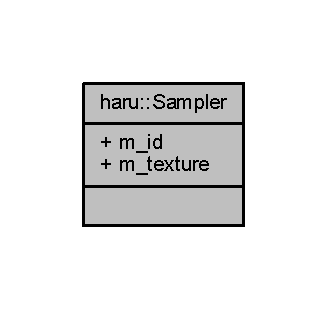
\includegraphics[width=157pt]{structharu_1_1_sampler__coll__graph}
\end{center}
\end{figure}
\subsection*{Public Attributes}
\begin{DoxyCompactItemize}
\item 
G\+Lint \mbox{\hyperlink{structharu_1_1_sampler_a363e0a0661392660270c1fdc356dcee7}{m\+\_\+id}}
\item 
std\+::shared\+\_\+ptr$<$ \mbox{\hyperlink{classharu_1_1_texture}{Texture}} $>$ \mbox{\hyperlink{structharu_1_1_sampler_a63c7dfdf6db2dd4ab18c1014ff7044af}{m\+\_\+texture}}
\end{DoxyCompactItemize}


\subsection{Member Data Documentation}
\mbox{\Hypertarget{structharu_1_1_sampler_a363e0a0661392660270c1fdc356dcee7}\label{structharu_1_1_sampler_a363e0a0661392660270c1fdc356dcee7}} 
\index{haru\+::\+Sampler@{haru\+::\+Sampler}!m\+\_\+id@{m\+\_\+id}}
\index{m\+\_\+id@{m\+\_\+id}!haru\+::\+Sampler@{haru\+::\+Sampler}}
\subsubsection{\texorpdfstring{m\+\_\+id}{m\_id}}
{\footnotesize\ttfamily G\+Lint haru\+::\+Sampler\+::m\+\_\+id}

\mbox{\Hypertarget{structharu_1_1_sampler_a63c7dfdf6db2dd4ab18c1014ff7044af}\label{structharu_1_1_sampler_a63c7dfdf6db2dd4ab18c1014ff7044af}} 
\index{haru\+::\+Sampler@{haru\+::\+Sampler}!m\+\_\+texture@{m\+\_\+texture}}
\index{m\+\_\+texture@{m\+\_\+texture}!haru\+::\+Sampler@{haru\+::\+Sampler}}
\subsubsection{\texorpdfstring{m\+\_\+texture}{m\_texture}}
{\footnotesize\ttfamily std\+::shared\+\_\+ptr$<$\mbox{\hyperlink{classharu_1_1_texture}{Texture}}$>$ haru\+::\+Sampler\+::m\+\_\+texture}



The documentation for this struct was generated from the following file\+:\begin{DoxyCompactItemize}
\item 
source/haruengine/\mbox{\hyperlink{_shader_program_8h}{Shader\+Program.\+h}}\end{DoxyCompactItemize}

\hypertarget{classharu_1_1_segment}{}\section{haru\+:\+:Segment Class Reference}
\label{classharu_1_1_segment}\index{haru\+::\+Segment@{haru\+::\+Segment}}


{\ttfamily \#include $<$Segment.\+h$>$}



Inheritance diagram for haru\+:\+:Segment\+:\nopagebreak
\begin{figure}[H]
\begin{center}
\leavevmode
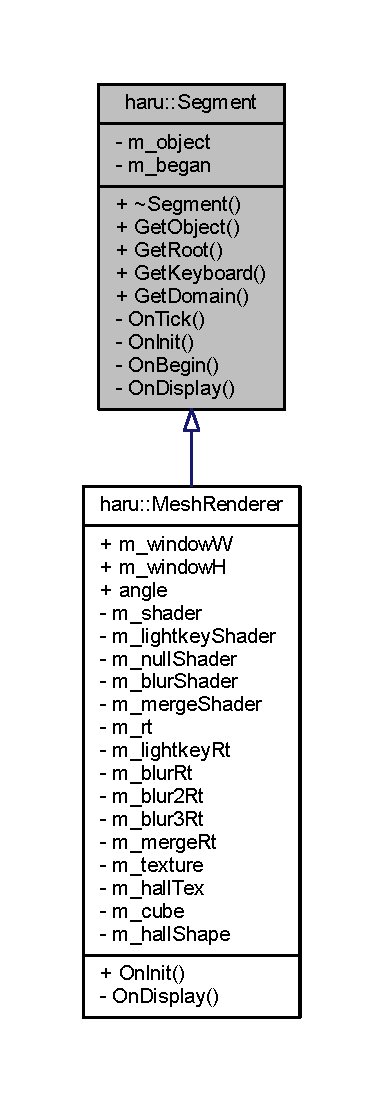
\includegraphics[width=184pt]{classharu_1_1_segment__inherit__graph}
\end{center}
\end{figure}


Collaboration diagram for haru\+:\+:Segment\+:\nopagebreak
\begin{figure}[H]
\begin{center}
\leavevmode
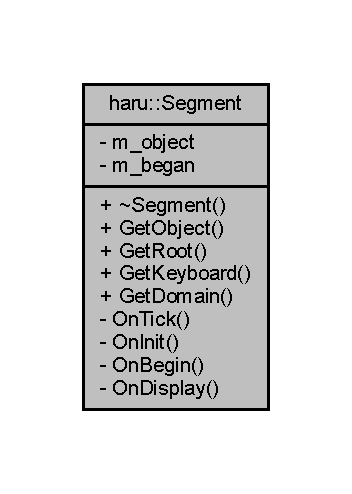
\includegraphics[width=169pt]{classharu_1_1_segment__coll__graph}
\end{center}
\end{figure}
\subsection*{Public Member Functions}
\begin{DoxyCompactItemize}
\item 
virtual \mbox{\hyperlink{classharu_1_1_segment_ac21fa3784567cb3c94280c40f4c006ba}{$\sim$\+Segment}} ()
\item 
std\+::shared\+\_\+ptr$<$ \mbox{\hyperlink{classharu_1_1_object}{Object}} $>$ \mbox{\hyperlink{classharu_1_1_segment_ae4262d0dbfca541db24d43e8925e9d8a}{Get\+Object}} ()
\item 
std\+::shared\+\_\+ptr$<$ \mbox{\hyperlink{classharu_1_1_root}{Root}} $>$ \mbox{\hyperlink{classharu_1_1_segment_adf664884cf9c2b20fc3c8b6944f1ff63}{Get\+Root}} ()
\item 
std\+::shared\+\_\+ptr$<$ \mbox{\hyperlink{class_keyboard}{Keyboard}} $>$ \mbox{\hyperlink{classharu_1_1_segment_ad33423dcc7119727b1fd2cd2a70ecdbf}{Get\+Keyboard}} ()
\item 
std\+::shared\+\_\+ptr$<$ \mbox{\hyperlink{class_domain}{Domain}} $>$ \mbox{\hyperlink{classharu_1_1_segment_ab00d15d78e1d3ae9f3199fd90ef52dcb}{Get\+Domain}} ()
\end{DoxyCompactItemize}
\subsection*{Private Member Functions}
\begin{DoxyCompactItemize}
\item 
virtual void \mbox{\hyperlink{classharu_1_1_segment_ad8b0861ccbf13afe613ff07622c1507b}{On\+Tick}} ()
\item 
virtual void \mbox{\hyperlink{classharu_1_1_segment_adc41c8e5769e0057ade94abf669c6dbc}{On\+Init}} ()
\item 
virtual void \mbox{\hyperlink{classharu_1_1_segment_aa628559af83f147fbc9d1aa468918e55}{On\+Begin}} ()
\item 
virtual void \mbox{\hyperlink{classharu_1_1_segment_a5bb0f5cf9aecda465804016d3ed4092c}{On\+Display}} ()
\end{DoxyCompactItemize}
\subsection*{Private Attributes}
\begin{DoxyCompactItemize}
\item 
std\+::weak\+\_\+ptr$<$ \mbox{\hyperlink{classharu_1_1_object}{Object}} $>$ \mbox{\hyperlink{classharu_1_1_segment_af7740dcdd156244b9b1ac2cba85b6120}{m\+\_\+object}}
\item 
bool \mbox{\hyperlink{classharu_1_1_segment_a57c2851dcf8880898a1175b3fe25bae7}{m\+\_\+began}}
\end{DoxyCompactItemize}
\subsection*{Friends}
\begin{DoxyCompactItemize}
\item 
class \mbox{\hyperlink{classharu_1_1_segment_a0720b5f434e636e22a3ed34f847eec57}{Object}}
\end{DoxyCompactItemize}


\subsection{Constructor \& Destructor Documentation}
\mbox{\Hypertarget{classharu_1_1_segment_ac21fa3784567cb3c94280c40f4c006ba}\label{classharu_1_1_segment_ac21fa3784567cb3c94280c40f4c006ba}} 
\index{haru\+::\+Segment@{haru\+::\+Segment}!````~Segment@{$\sim$\+Segment}}
\index{````~Segment@{$\sim$\+Segment}!haru\+::\+Segment@{haru\+::\+Segment}}
\subsubsection{\texorpdfstring{$\sim$\+Segment()}{~Segment()}}
{\footnotesize\ttfamily haru\+::\+Segment\+::$\sim$\+Segment (\begin{DoxyParamCaption}{ }\end{DoxyParamCaption})\hspace{0.3cm}{\ttfamily [virtual]}}



\subsection{Member Function Documentation}
\mbox{\Hypertarget{classharu_1_1_segment_ab00d15d78e1d3ae9f3199fd90ef52dcb}\label{classharu_1_1_segment_ab00d15d78e1d3ae9f3199fd90ef52dcb}} 
\index{haru\+::\+Segment@{haru\+::\+Segment}!Get\+Domain@{Get\+Domain}}
\index{Get\+Domain@{Get\+Domain}!haru\+::\+Segment@{haru\+::\+Segment}}
\subsubsection{\texorpdfstring{Get\+Domain()}{GetDomain()}}
{\footnotesize\ttfamily std\+::shared\+\_\+ptr$<$ \mbox{\hyperlink{class_domain}{Domain}} $>$ haru\+::\+Segment\+::\+Get\+Domain (\begin{DoxyParamCaption}{ }\end{DoxyParamCaption})}

\mbox{\Hypertarget{classharu_1_1_segment_ad33423dcc7119727b1fd2cd2a70ecdbf}\label{classharu_1_1_segment_ad33423dcc7119727b1fd2cd2a70ecdbf}} 
\index{haru\+::\+Segment@{haru\+::\+Segment}!Get\+Keyboard@{Get\+Keyboard}}
\index{Get\+Keyboard@{Get\+Keyboard}!haru\+::\+Segment@{haru\+::\+Segment}}
\subsubsection{\texorpdfstring{Get\+Keyboard()}{GetKeyboard()}}
{\footnotesize\ttfamily std\+::shared\+\_\+ptr$<$ \mbox{\hyperlink{class_keyboard}{Keyboard}} $>$ haru\+::\+Segment\+::\+Get\+Keyboard (\begin{DoxyParamCaption}{ }\end{DoxyParamCaption})}

\mbox{\Hypertarget{classharu_1_1_segment_ae4262d0dbfca541db24d43e8925e9d8a}\label{classharu_1_1_segment_ae4262d0dbfca541db24d43e8925e9d8a}} 
\index{haru\+::\+Segment@{haru\+::\+Segment}!Get\+Object@{Get\+Object}}
\index{Get\+Object@{Get\+Object}!haru\+::\+Segment@{haru\+::\+Segment}}
\subsubsection{\texorpdfstring{Get\+Object()}{GetObject()}}
{\footnotesize\ttfamily std\+::shared\+\_\+ptr$<$ \mbox{\hyperlink{classharu_1_1_object}{Object}} $>$ haru\+::\+Segment\+::\+Get\+Object (\begin{DoxyParamCaption}{ }\end{DoxyParamCaption})}

Here is the caller graph for this function\+:
\nopagebreak
\begin{figure}[H]
\begin{center}
\leavevmode
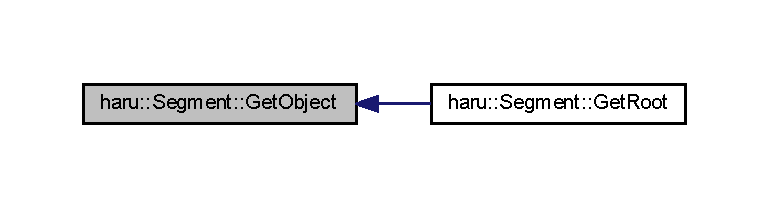
\includegraphics[width=350pt]{classharu_1_1_segment_ae4262d0dbfca541db24d43e8925e9d8a_icgraph}
\end{center}
\end{figure}
\mbox{\Hypertarget{classharu_1_1_segment_adf664884cf9c2b20fc3c8b6944f1ff63}\label{classharu_1_1_segment_adf664884cf9c2b20fc3c8b6944f1ff63}} 
\index{haru\+::\+Segment@{haru\+::\+Segment}!Get\+Root@{Get\+Root}}
\index{Get\+Root@{Get\+Root}!haru\+::\+Segment@{haru\+::\+Segment}}
\subsubsection{\texorpdfstring{Get\+Root()}{GetRoot()}}
{\footnotesize\ttfamily std\+::shared\+\_\+ptr$<$ \mbox{\hyperlink{classharu_1_1_root}{Root}} $>$ haru\+::\+Segment\+::\+Get\+Root (\begin{DoxyParamCaption}{ }\end{DoxyParamCaption})}

Here is the call graph for this function\+:
\nopagebreak
\begin{figure}[H]
\begin{center}
\leavevmode
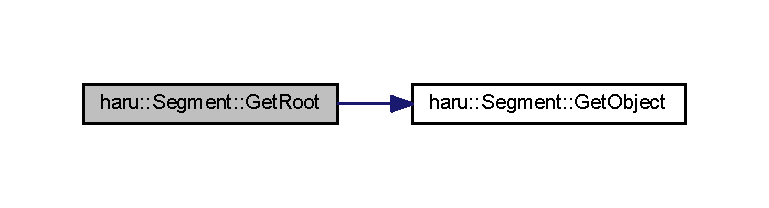
\includegraphics[width=350pt]{classharu_1_1_segment_adf664884cf9c2b20fc3c8b6944f1ff63_cgraph}
\end{center}
\end{figure}
\mbox{\Hypertarget{classharu_1_1_segment_aa628559af83f147fbc9d1aa468918e55}\label{classharu_1_1_segment_aa628559af83f147fbc9d1aa468918e55}} 
\index{haru\+::\+Segment@{haru\+::\+Segment}!On\+Begin@{On\+Begin}}
\index{On\+Begin@{On\+Begin}!haru\+::\+Segment@{haru\+::\+Segment}}
\subsubsection{\texorpdfstring{On\+Begin()}{OnBegin()}}
{\footnotesize\ttfamily void haru\+::\+Segment\+::\+On\+Begin (\begin{DoxyParamCaption}{ }\end{DoxyParamCaption})\hspace{0.3cm}{\ttfamily [private]}, {\ttfamily [virtual]}}

\mbox{\Hypertarget{classharu_1_1_segment_a5bb0f5cf9aecda465804016d3ed4092c}\label{classharu_1_1_segment_a5bb0f5cf9aecda465804016d3ed4092c}} 
\index{haru\+::\+Segment@{haru\+::\+Segment}!On\+Display@{On\+Display}}
\index{On\+Display@{On\+Display}!haru\+::\+Segment@{haru\+::\+Segment}}
\subsubsection{\texorpdfstring{On\+Display()}{OnDisplay()}}
{\footnotesize\ttfamily void haru\+::\+Segment\+::\+On\+Display (\begin{DoxyParamCaption}{ }\end{DoxyParamCaption})\hspace{0.3cm}{\ttfamily [private]}, {\ttfamily [virtual]}}



Reimplemented in \mbox{\hyperlink{classharu_1_1_mesh_renderer_ac927c9cc1d392ca8305ca995ddc0b7a6}{haru\+::\+Mesh\+Renderer}}.

\mbox{\Hypertarget{classharu_1_1_segment_adc41c8e5769e0057ade94abf669c6dbc}\label{classharu_1_1_segment_adc41c8e5769e0057ade94abf669c6dbc}} 
\index{haru\+::\+Segment@{haru\+::\+Segment}!On\+Init@{On\+Init}}
\index{On\+Init@{On\+Init}!haru\+::\+Segment@{haru\+::\+Segment}}
\subsubsection{\texorpdfstring{On\+Init()}{OnInit()}}
{\footnotesize\ttfamily void haru\+::\+Segment\+::\+On\+Init (\begin{DoxyParamCaption}{ }\end{DoxyParamCaption})\hspace{0.3cm}{\ttfamily [private]}, {\ttfamily [virtual]}}



Reimplemented in \mbox{\hyperlink{classharu_1_1_mesh_renderer_a5a6a5b945fc7560d166e9d16058aec53}{haru\+::\+Mesh\+Renderer}}.

\mbox{\Hypertarget{classharu_1_1_segment_ad8b0861ccbf13afe613ff07622c1507b}\label{classharu_1_1_segment_ad8b0861ccbf13afe613ff07622c1507b}} 
\index{haru\+::\+Segment@{haru\+::\+Segment}!On\+Tick@{On\+Tick}}
\index{On\+Tick@{On\+Tick}!haru\+::\+Segment@{haru\+::\+Segment}}
\subsubsection{\texorpdfstring{On\+Tick()}{OnTick()}}
{\footnotesize\ttfamily void haru\+::\+Segment\+::\+On\+Tick (\begin{DoxyParamCaption}{ }\end{DoxyParamCaption})\hspace{0.3cm}{\ttfamily [private]}, {\ttfamily [virtual]}}



\subsection{Friends And Related Function Documentation}
\mbox{\Hypertarget{classharu_1_1_segment_a0720b5f434e636e22a3ed34f847eec57}\label{classharu_1_1_segment_a0720b5f434e636e22a3ed34f847eec57}} 
\index{haru\+::\+Segment@{haru\+::\+Segment}!Object@{Object}}
\index{Object@{Object}!haru\+::\+Segment@{haru\+::\+Segment}}
\subsubsection{\texorpdfstring{Object}{Object}}
{\footnotesize\ttfamily friend class \mbox{\hyperlink{classharu_1_1_object}{Object}}\hspace{0.3cm}{\ttfamily [friend]}}



\subsection{Member Data Documentation}
\mbox{\Hypertarget{classharu_1_1_segment_a57c2851dcf8880898a1175b3fe25bae7}\label{classharu_1_1_segment_a57c2851dcf8880898a1175b3fe25bae7}} 
\index{haru\+::\+Segment@{haru\+::\+Segment}!m\+\_\+began@{m\+\_\+began}}
\index{m\+\_\+began@{m\+\_\+began}!haru\+::\+Segment@{haru\+::\+Segment}}
\subsubsection{\texorpdfstring{m\+\_\+began}{m\_began}}
{\footnotesize\ttfamily bool haru\+::\+Segment\+::m\+\_\+began\hspace{0.3cm}{\ttfamily [private]}}

\mbox{\Hypertarget{classharu_1_1_segment_af7740dcdd156244b9b1ac2cba85b6120}\label{classharu_1_1_segment_af7740dcdd156244b9b1ac2cba85b6120}} 
\index{haru\+::\+Segment@{haru\+::\+Segment}!m\+\_\+object@{m\+\_\+object}}
\index{m\+\_\+object@{m\+\_\+object}!haru\+::\+Segment@{haru\+::\+Segment}}
\subsubsection{\texorpdfstring{m\+\_\+object}{m\_object}}
{\footnotesize\ttfamily std\+::weak\+\_\+ptr$<$\mbox{\hyperlink{classharu_1_1_object}{Object}}$>$ haru\+::\+Segment\+::m\+\_\+object\hspace{0.3cm}{\ttfamily [private]}}



The documentation for this class was generated from the following files\+:\begin{DoxyCompactItemize}
\item 
source/haruengine/\mbox{\hyperlink{_segment_8h}{Segment.\+h}}\item 
source/haruengine/\mbox{\hyperlink{_segment_8cpp}{Segment.\+cpp}}\end{DoxyCompactItemize}

\hypertarget{classharu_1_1_shader_program}{}\section{haru\+:\+:Shader\+Program Class Reference}
\label{classharu_1_1_shader_program}\index{haru\+::\+Shader\+Program@{haru\+::\+Shader\+Program}}


{\ttfamily \#include $<$Shader\+Program.\+h$>$}



Collaboration diagram for haru\+:\+:Shader\+Program\+:\nopagebreak
\begin{figure}[H]
\begin{center}
\leavevmode
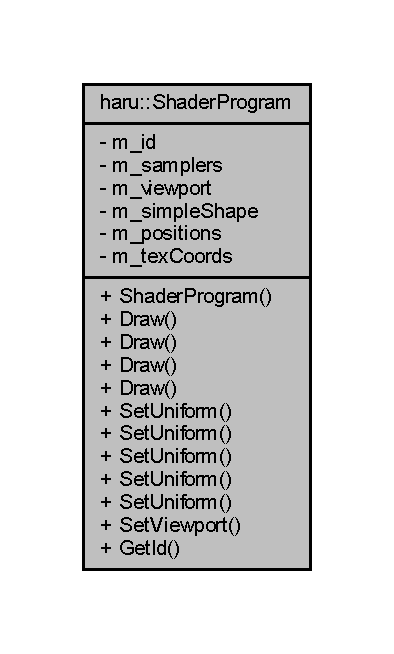
\includegraphics[width=189pt]{classharu_1_1_shader_program__coll__graph}
\end{center}
\end{figure}
\subsection*{Public Member Functions}
\begin{DoxyCompactItemize}
\item 
\mbox{\hyperlink{classharu_1_1_shader_program_acfb9528364468c5cbabb1f581643ae25}{Shader\+Program}} (std\+::string \+\_\+vert, std\+::string \+\_\+frag)
\item 
void \mbox{\hyperlink{classharu_1_1_shader_program_ab23193ba8426b49073e64646b7de6320}{Draw}} ()
\item 
void \mbox{\hyperlink{classharu_1_1_shader_program_a6e322ac38c9358486ccee3c06aef4de1}{Draw}} (std\+::shared\+\_\+ptr$<$ \mbox{\hyperlink{classharu_1_1_render_texture}{Render\+Texture}} $>$ \+\_\+render\+Texture)
\item 
void \mbox{\hyperlink{classharu_1_1_shader_program_af76596f322a345e67ad8ee1395cc76c4}{Draw}} (std\+::shared\+\_\+ptr$<$ \mbox{\hyperlink{classharu_1_1_vertex_array}{Vertex\+Array}} $>$ \+\_\+vertex\+Array)
\item 
void \mbox{\hyperlink{classharu_1_1_shader_program_af06e97b4b8eec4d8fd197f58df319206}{Draw}} (std\+::shared\+\_\+ptr$<$ \mbox{\hyperlink{classharu_1_1_render_texture}{Render\+Texture}} $>$ \+\_\+render\+Texture, std\+::shared\+\_\+ptr$<$ \mbox{\hyperlink{classharu_1_1_vertex_array}{Vertex\+Array}} $>$ \+\_\+vertex\+Array)
\item 
void \mbox{\hyperlink{classharu_1_1_shader_program_a558038555953abdd400d17b6af6a821b}{Set\+Uniform}} (std\+::string \+\_\+uniform, glm\+::vec4 \+\_\+value)
\item 
void \mbox{\hyperlink{classharu_1_1_shader_program_abd818797df7d006a1d8d2646653e576a}{Set\+Uniform}} (std\+::string \+\_\+uniform, float \+\_\+value)
\item 
void \mbox{\hyperlink{classharu_1_1_shader_program_a6cdbf2ff9c5bce4b7b1c039a1d9af142}{Set\+Uniform}} (std\+::string \+\_\+uniform, int \+\_\+value)
\item 
void \mbox{\hyperlink{classharu_1_1_shader_program_a9d36534e1ffd87f185da4b2bb7945723}{Set\+Uniform}} (std\+::string \+\_\+uniform, glm\+::mat4 \+\_\+value)
\item 
void \mbox{\hyperlink{classharu_1_1_shader_program_a9ea7128d64215e9e79076a0b36a69849}{Set\+Uniform}} (std\+::string \+\_\+uniform, std\+::shared\+\_\+ptr$<$ \mbox{\hyperlink{classharu_1_1_texture}{Texture}} $>$ \+\_\+texture)
\item 
void \mbox{\hyperlink{classharu_1_1_shader_program_a9534e78aa5537cf3e7f63a7c8d166ba7}{Set\+Viewport}} (glm\+::vec4 \+\_\+viewport)
\item 
G\+Luint \mbox{\hyperlink{classharu_1_1_shader_program_a6079bce91bd203b0915d974035701cfd}{Get\+Id}} ()
\end{DoxyCompactItemize}
\subsection*{Private Attributes}
\begin{DoxyCompactItemize}
\item 
G\+Luint \mbox{\hyperlink{classharu_1_1_shader_program_a9aefbe81aaa09ee5d881c708d14c4175}{m\+\_\+id}}
\item 
std\+::vector$<$ \mbox{\hyperlink{structharu_1_1_sampler}{Sampler}} $>$ \mbox{\hyperlink{classharu_1_1_shader_program_acb7b3e2ef877a1022fccf4951567d1bf}{m\+\_\+samplers}}
\item 
glm\+::vec4 \mbox{\hyperlink{classharu_1_1_shader_program_a2eb3daf1a2dc547187d934a5db92ab6a}{m\+\_\+viewport}}
\item 
std\+::shared\+\_\+ptr$<$ \mbox{\hyperlink{classharu_1_1_vertex_array}{Vertex\+Array}} $>$ \mbox{\hyperlink{classharu_1_1_shader_program_a294aa6017a95424af663d11de22c8a30}{m\+\_\+simple\+Shape}}
\item 
std\+::shared\+\_\+ptr$<$ \mbox{\hyperlink{classharu_1_1_vertex_buffer}{Vertex\+Buffer}} $>$ \mbox{\hyperlink{classharu_1_1_shader_program_a2c35054cf33234db86676f9c94bef3a6}{m\+\_\+positions}}
\item 
std\+::shared\+\_\+ptr$<$ \mbox{\hyperlink{classharu_1_1_vertex_buffer}{Vertex\+Buffer}} $>$ \mbox{\hyperlink{classharu_1_1_shader_program_acbf6bb784e05081a29ef90a04ae2269d}{m\+\_\+tex\+Coords}}
\end{DoxyCompactItemize}


\subsection{Constructor \& Destructor Documentation}
\mbox{\Hypertarget{classharu_1_1_shader_program_acfb9528364468c5cbabb1f581643ae25}\label{classharu_1_1_shader_program_acfb9528364468c5cbabb1f581643ae25}} 
\index{haru\+::\+Shader\+Program@{haru\+::\+Shader\+Program}!Shader\+Program@{Shader\+Program}}
\index{Shader\+Program@{Shader\+Program}!haru\+::\+Shader\+Program@{haru\+::\+Shader\+Program}}
\subsubsection{\texorpdfstring{Shader\+Program()}{ShaderProgram()}}
{\footnotesize\ttfamily haru\+::\+Shader\+Program\+::\+Shader\+Program (\begin{DoxyParamCaption}\item[{std\+::string}]{\+\_\+vert,  }\item[{std\+::string}]{\+\_\+frag }\end{DoxyParamCaption})}



\subsection{Member Function Documentation}
\mbox{\Hypertarget{classharu_1_1_shader_program_ab23193ba8426b49073e64646b7de6320}\label{classharu_1_1_shader_program_ab23193ba8426b49073e64646b7de6320}} 
\index{haru\+::\+Shader\+Program@{haru\+::\+Shader\+Program}!Draw@{Draw}}
\index{Draw@{Draw}!haru\+::\+Shader\+Program@{haru\+::\+Shader\+Program}}
\subsubsection{\texorpdfstring{Draw()}{Draw()}\hspace{0.1cm}{\footnotesize\ttfamily [1/4]}}
{\footnotesize\ttfamily void haru\+::\+Shader\+Program\+::\+Draw (\begin{DoxyParamCaption}{ }\end{DoxyParamCaption})}

Here is the caller graph for this function\+:
\nopagebreak
\begin{figure}[H]
\begin{center}
\leavevmode
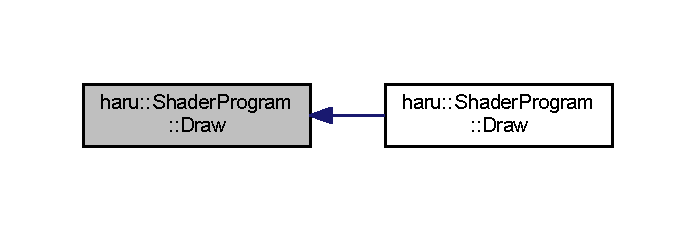
\includegraphics[width=334pt]{classharu_1_1_shader_program_ab23193ba8426b49073e64646b7de6320_icgraph}
\end{center}
\end{figure}
\mbox{\Hypertarget{classharu_1_1_shader_program_a6e322ac38c9358486ccee3c06aef4de1}\label{classharu_1_1_shader_program_a6e322ac38c9358486ccee3c06aef4de1}} 
\index{haru\+::\+Shader\+Program@{haru\+::\+Shader\+Program}!Draw@{Draw}}
\index{Draw@{Draw}!haru\+::\+Shader\+Program@{haru\+::\+Shader\+Program}}
\subsubsection{\texorpdfstring{Draw()}{Draw()}\hspace{0.1cm}{\footnotesize\ttfamily [2/4]}}
{\footnotesize\ttfamily void haru\+::\+Shader\+Program\+::\+Draw (\begin{DoxyParamCaption}\item[{std\+::shared\+\_\+ptr$<$ \mbox{\hyperlink{classharu_1_1_render_texture}{Render\+Texture}} $>$}]{\+\_\+render\+Texture }\end{DoxyParamCaption})}

Here is the call graph for this function\+:
\nopagebreak
\begin{figure}[H]
\begin{center}
\leavevmode
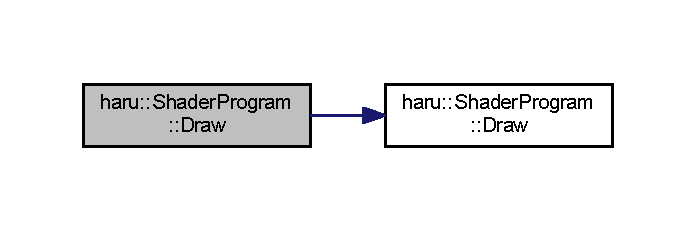
\includegraphics[width=334pt]{classharu_1_1_shader_program_a6e322ac38c9358486ccee3c06aef4de1_cgraph}
\end{center}
\end{figure}
\mbox{\Hypertarget{classharu_1_1_shader_program_af76596f322a345e67ad8ee1395cc76c4}\label{classharu_1_1_shader_program_af76596f322a345e67ad8ee1395cc76c4}} 
\index{haru\+::\+Shader\+Program@{haru\+::\+Shader\+Program}!Draw@{Draw}}
\index{Draw@{Draw}!haru\+::\+Shader\+Program@{haru\+::\+Shader\+Program}}
\subsubsection{\texorpdfstring{Draw()}{Draw()}\hspace{0.1cm}{\footnotesize\ttfamily [3/4]}}
{\footnotesize\ttfamily void haru\+::\+Shader\+Program\+::\+Draw (\begin{DoxyParamCaption}\item[{std\+::shared\+\_\+ptr$<$ \mbox{\hyperlink{classharu_1_1_vertex_array}{Vertex\+Array}} $>$}]{\+\_\+vertex\+Array }\end{DoxyParamCaption})}

\mbox{\Hypertarget{classharu_1_1_shader_program_af06e97b4b8eec4d8fd197f58df319206}\label{classharu_1_1_shader_program_af06e97b4b8eec4d8fd197f58df319206}} 
\index{haru\+::\+Shader\+Program@{haru\+::\+Shader\+Program}!Draw@{Draw}}
\index{Draw@{Draw}!haru\+::\+Shader\+Program@{haru\+::\+Shader\+Program}}
\subsubsection{\texorpdfstring{Draw()}{Draw()}\hspace{0.1cm}{\footnotesize\ttfamily [4/4]}}
{\footnotesize\ttfamily void haru\+::\+Shader\+Program\+::\+Draw (\begin{DoxyParamCaption}\item[{std\+::shared\+\_\+ptr$<$ \mbox{\hyperlink{classharu_1_1_render_texture}{Render\+Texture}} $>$}]{\+\_\+render\+Texture,  }\item[{std\+::shared\+\_\+ptr$<$ \mbox{\hyperlink{classharu_1_1_vertex_array}{Vertex\+Array}} $>$}]{\+\_\+vertex\+Array }\end{DoxyParamCaption})}

Here is the call graph for this function\+:
\nopagebreak
\begin{figure}[H]
\begin{center}
\leavevmode
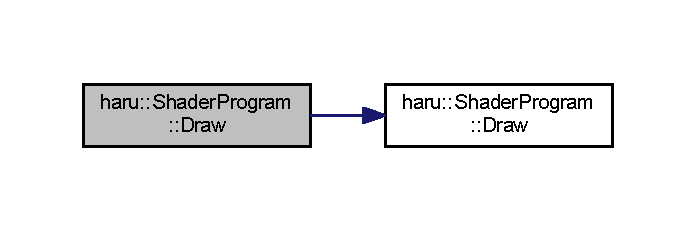
\includegraphics[width=334pt]{classharu_1_1_shader_program_af06e97b4b8eec4d8fd197f58df319206_cgraph}
\end{center}
\end{figure}
\mbox{\Hypertarget{classharu_1_1_shader_program_a6079bce91bd203b0915d974035701cfd}\label{classharu_1_1_shader_program_a6079bce91bd203b0915d974035701cfd}} 
\index{haru\+::\+Shader\+Program@{haru\+::\+Shader\+Program}!Get\+Id@{Get\+Id}}
\index{Get\+Id@{Get\+Id}!haru\+::\+Shader\+Program@{haru\+::\+Shader\+Program}}
\subsubsection{\texorpdfstring{Get\+Id()}{GetId()}}
{\footnotesize\ttfamily G\+Luint haru\+::\+Shader\+Program\+::\+Get\+Id (\begin{DoxyParamCaption}{ }\end{DoxyParamCaption})}

\mbox{\Hypertarget{classharu_1_1_shader_program_a558038555953abdd400d17b6af6a821b}\label{classharu_1_1_shader_program_a558038555953abdd400d17b6af6a821b}} 
\index{haru\+::\+Shader\+Program@{haru\+::\+Shader\+Program}!Set\+Uniform@{Set\+Uniform}}
\index{Set\+Uniform@{Set\+Uniform}!haru\+::\+Shader\+Program@{haru\+::\+Shader\+Program}}
\subsubsection{\texorpdfstring{Set\+Uniform()}{SetUniform()}\hspace{0.1cm}{\footnotesize\ttfamily [1/5]}}
{\footnotesize\ttfamily void haru\+::\+Shader\+Program\+::\+Set\+Uniform (\begin{DoxyParamCaption}\item[{std\+::string}]{\+\_\+uniform,  }\item[{glm\+::vec4}]{\+\_\+value }\end{DoxyParamCaption})}

\mbox{\Hypertarget{classharu_1_1_shader_program_abd818797df7d006a1d8d2646653e576a}\label{classharu_1_1_shader_program_abd818797df7d006a1d8d2646653e576a}} 
\index{haru\+::\+Shader\+Program@{haru\+::\+Shader\+Program}!Set\+Uniform@{Set\+Uniform}}
\index{Set\+Uniform@{Set\+Uniform}!haru\+::\+Shader\+Program@{haru\+::\+Shader\+Program}}
\subsubsection{\texorpdfstring{Set\+Uniform()}{SetUniform()}\hspace{0.1cm}{\footnotesize\ttfamily [2/5]}}
{\footnotesize\ttfamily void haru\+::\+Shader\+Program\+::\+Set\+Uniform (\begin{DoxyParamCaption}\item[{std\+::string}]{\+\_\+uniform,  }\item[{float}]{\+\_\+value }\end{DoxyParamCaption})}

\mbox{\Hypertarget{classharu_1_1_shader_program_a6cdbf2ff9c5bce4b7b1c039a1d9af142}\label{classharu_1_1_shader_program_a6cdbf2ff9c5bce4b7b1c039a1d9af142}} 
\index{haru\+::\+Shader\+Program@{haru\+::\+Shader\+Program}!Set\+Uniform@{Set\+Uniform}}
\index{Set\+Uniform@{Set\+Uniform}!haru\+::\+Shader\+Program@{haru\+::\+Shader\+Program}}
\subsubsection{\texorpdfstring{Set\+Uniform()}{SetUniform()}\hspace{0.1cm}{\footnotesize\ttfamily [3/5]}}
{\footnotesize\ttfamily void haru\+::\+Shader\+Program\+::\+Set\+Uniform (\begin{DoxyParamCaption}\item[{std\+::string}]{\+\_\+uniform,  }\item[{int}]{\+\_\+value }\end{DoxyParamCaption})}

\mbox{\Hypertarget{classharu_1_1_shader_program_a9d36534e1ffd87f185da4b2bb7945723}\label{classharu_1_1_shader_program_a9d36534e1ffd87f185da4b2bb7945723}} 
\index{haru\+::\+Shader\+Program@{haru\+::\+Shader\+Program}!Set\+Uniform@{Set\+Uniform}}
\index{Set\+Uniform@{Set\+Uniform}!haru\+::\+Shader\+Program@{haru\+::\+Shader\+Program}}
\subsubsection{\texorpdfstring{Set\+Uniform()}{SetUniform()}\hspace{0.1cm}{\footnotesize\ttfamily [4/5]}}
{\footnotesize\ttfamily void haru\+::\+Shader\+Program\+::\+Set\+Uniform (\begin{DoxyParamCaption}\item[{std\+::string}]{\+\_\+uniform,  }\item[{glm\+::mat4}]{\+\_\+value }\end{DoxyParamCaption})}

\mbox{\Hypertarget{classharu_1_1_shader_program_a9ea7128d64215e9e79076a0b36a69849}\label{classharu_1_1_shader_program_a9ea7128d64215e9e79076a0b36a69849}} 
\index{haru\+::\+Shader\+Program@{haru\+::\+Shader\+Program}!Set\+Uniform@{Set\+Uniform}}
\index{Set\+Uniform@{Set\+Uniform}!haru\+::\+Shader\+Program@{haru\+::\+Shader\+Program}}
\subsubsection{\texorpdfstring{Set\+Uniform()}{SetUniform()}\hspace{0.1cm}{\footnotesize\ttfamily [5/5]}}
{\footnotesize\ttfamily void haru\+::\+Shader\+Program\+::\+Set\+Uniform (\begin{DoxyParamCaption}\item[{std\+::string}]{\+\_\+uniform,  }\item[{std\+::shared\+\_\+ptr$<$ \mbox{\hyperlink{classharu_1_1_texture}{Texture}} $>$}]{\+\_\+texture }\end{DoxyParamCaption})}

\mbox{\Hypertarget{classharu_1_1_shader_program_a9534e78aa5537cf3e7f63a7c8d166ba7}\label{classharu_1_1_shader_program_a9534e78aa5537cf3e7f63a7c8d166ba7}} 
\index{haru\+::\+Shader\+Program@{haru\+::\+Shader\+Program}!Set\+Viewport@{Set\+Viewport}}
\index{Set\+Viewport@{Set\+Viewport}!haru\+::\+Shader\+Program@{haru\+::\+Shader\+Program}}
\subsubsection{\texorpdfstring{Set\+Viewport()}{SetViewport()}}
{\footnotesize\ttfamily void haru\+::\+Shader\+Program\+::\+Set\+Viewport (\begin{DoxyParamCaption}\item[{glm\+::vec4}]{\+\_\+viewport }\end{DoxyParamCaption})}



\subsection{Member Data Documentation}
\mbox{\Hypertarget{classharu_1_1_shader_program_a9aefbe81aaa09ee5d881c708d14c4175}\label{classharu_1_1_shader_program_a9aefbe81aaa09ee5d881c708d14c4175}} 
\index{haru\+::\+Shader\+Program@{haru\+::\+Shader\+Program}!m\+\_\+id@{m\+\_\+id}}
\index{m\+\_\+id@{m\+\_\+id}!haru\+::\+Shader\+Program@{haru\+::\+Shader\+Program}}
\subsubsection{\texorpdfstring{m\+\_\+id}{m\_id}}
{\footnotesize\ttfamily G\+Luint haru\+::\+Shader\+Program\+::m\+\_\+id\hspace{0.3cm}{\ttfamily [private]}}

\mbox{\Hypertarget{classharu_1_1_shader_program_a2c35054cf33234db86676f9c94bef3a6}\label{classharu_1_1_shader_program_a2c35054cf33234db86676f9c94bef3a6}} 
\index{haru\+::\+Shader\+Program@{haru\+::\+Shader\+Program}!m\+\_\+positions@{m\+\_\+positions}}
\index{m\+\_\+positions@{m\+\_\+positions}!haru\+::\+Shader\+Program@{haru\+::\+Shader\+Program}}
\subsubsection{\texorpdfstring{m\+\_\+positions}{m\_positions}}
{\footnotesize\ttfamily std\+::shared\+\_\+ptr$<$\mbox{\hyperlink{classharu_1_1_vertex_buffer}{Vertex\+Buffer}}$>$ haru\+::\+Shader\+Program\+::m\+\_\+positions\hspace{0.3cm}{\ttfamily [private]}}

\mbox{\Hypertarget{classharu_1_1_shader_program_acb7b3e2ef877a1022fccf4951567d1bf}\label{classharu_1_1_shader_program_acb7b3e2ef877a1022fccf4951567d1bf}} 
\index{haru\+::\+Shader\+Program@{haru\+::\+Shader\+Program}!m\+\_\+samplers@{m\+\_\+samplers}}
\index{m\+\_\+samplers@{m\+\_\+samplers}!haru\+::\+Shader\+Program@{haru\+::\+Shader\+Program}}
\subsubsection{\texorpdfstring{m\+\_\+samplers}{m\_samplers}}
{\footnotesize\ttfamily std\+::vector$<$\mbox{\hyperlink{structharu_1_1_sampler}{Sampler}}$>$ haru\+::\+Shader\+Program\+::m\+\_\+samplers\hspace{0.3cm}{\ttfamily [private]}}

\mbox{\Hypertarget{classharu_1_1_shader_program_a294aa6017a95424af663d11de22c8a30}\label{classharu_1_1_shader_program_a294aa6017a95424af663d11de22c8a30}} 
\index{haru\+::\+Shader\+Program@{haru\+::\+Shader\+Program}!m\+\_\+simple\+Shape@{m\+\_\+simple\+Shape}}
\index{m\+\_\+simple\+Shape@{m\+\_\+simple\+Shape}!haru\+::\+Shader\+Program@{haru\+::\+Shader\+Program}}
\subsubsection{\texorpdfstring{m\+\_\+simple\+Shape}{m\_simpleShape}}
{\footnotesize\ttfamily std\+::shared\+\_\+ptr$<$\mbox{\hyperlink{classharu_1_1_vertex_array}{Vertex\+Array}}$>$ haru\+::\+Shader\+Program\+::m\+\_\+simple\+Shape\hspace{0.3cm}{\ttfamily [private]}}

\mbox{\Hypertarget{classharu_1_1_shader_program_acbf6bb784e05081a29ef90a04ae2269d}\label{classharu_1_1_shader_program_acbf6bb784e05081a29ef90a04ae2269d}} 
\index{haru\+::\+Shader\+Program@{haru\+::\+Shader\+Program}!m\+\_\+tex\+Coords@{m\+\_\+tex\+Coords}}
\index{m\+\_\+tex\+Coords@{m\+\_\+tex\+Coords}!haru\+::\+Shader\+Program@{haru\+::\+Shader\+Program}}
\subsubsection{\texorpdfstring{m\+\_\+tex\+Coords}{m\_texCoords}}
{\footnotesize\ttfamily std\+::shared\+\_\+ptr$<$\mbox{\hyperlink{classharu_1_1_vertex_buffer}{Vertex\+Buffer}}$>$ haru\+::\+Shader\+Program\+::m\+\_\+tex\+Coords\hspace{0.3cm}{\ttfamily [private]}}

\mbox{\Hypertarget{classharu_1_1_shader_program_a2eb3daf1a2dc547187d934a5db92ab6a}\label{classharu_1_1_shader_program_a2eb3daf1a2dc547187d934a5db92ab6a}} 
\index{haru\+::\+Shader\+Program@{haru\+::\+Shader\+Program}!m\+\_\+viewport@{m\+\_\+viewport}}
\index{m\+\_\+viewport@{m\+\_\+viewport}!haru\+::\+Shader\+Program@{haru\+::\+Shader\+Program}}
\subsubsection{\texorpdfstring{m\+\_\+viewport}{m\_viewport}}
{\footnotesize\ttfamily glm\+::vec4 haru\+::\+Shader\+Program\+::m\+\_\+viewport\hspace{0.3cm}{\ttfamily [private]}}



The documentation for this class was generated from the following files\+:\begin{DoxyCompactItemize}
\item 
source/haruengine/\mbox{\hyperlink{_shader_program_8h}{Shader\+Program.\+h}}\item 
source/haruengine/\mbox{\hyperlink{_shader_program_8cpp}{Shader\+Program.\+cpp}}\end{DoxyCompactItemize}

\hypertarget{classharu_1_1_texture}{}\section{haru\+:\+:Texture Class Reference}
\label{classharu_1_1_texture}\index{haru\+::\+Texture@{haru\+::\+Texture}}


{\ttfamily \#include $<$Texture.\+h$>$}



Inheritance diagram for haru\+:\+:Texture\+:\nopagebreak
\begin{figure}[H]
\begin{center}
\leavevmode
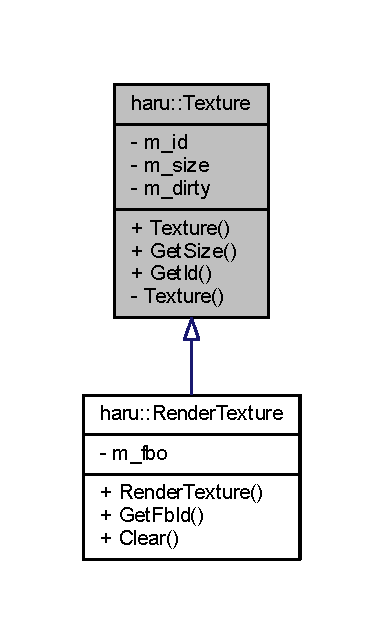
\includegraphics[width=184pt]{classharu_1_1_texture__inherit__graph}
\end{center}
\end{figure}


Collaboration diagram for haru\+:\+:Texture\+:\nopagebreak
\begin{figure}[H]
\begin{center}
\leavevmode
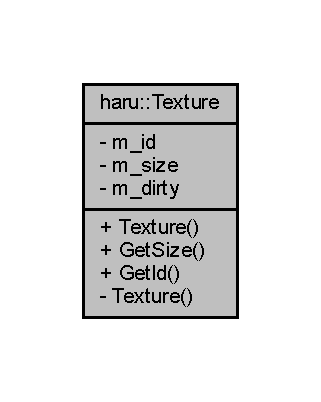
\includegraphics[width=154pt]{classharu_1_1_texture__coll__graph}
\end{center}
\end{figure}
\subsection*{Public Member Functions}
\begin{DoxyCompactItemize}
\item 
\mbox{\hyperlink{classharu_1_1_texture_a422b89c2d2b128a0ceb835c33134ec5f}{Texture}} (std\+::string \+\_\+path)
\item 
glm\+::vec2 \mbox{\hyperlink{classharu_1_1_texture_a8ca167a24b26121d9f4547c4a947693c}{Get\+Size}} ()
\item 
G\+Luint \mbox{\hyperlink{classharu_1_1_texture_aaf9f37304ea11cec8c9a4400850f314d}{Get\+Id}} ()
\end{DoxyCompactItemize}
\subsection*{Private Member Functions}
\begin{DoxyCompactItemize}
\item 
\mbox{\hyperlink{classharu_1_1_texture_a088277a42ce0ffa25e5df90856d2a70b}{Texture}} (int \+\_\+width, int \+\_\+height)
\end{DoxyCompactItemize}
\subsection*{Private Attributes}
\begin{DoxyCompactItemize}
\item 
G\+Luint \mbox{\hyperlink{classharu_1_1_texture_a7fe6446509151f52d72bb1c18a06cc7b}{m\+\_\+id}}
\item 
glm\+::vec2 \mbox{\hyperlink{classharu_1_1_texture_a8a15e433e4eef90ef52bb2243b91ef00}{m\+\_\+size}}
\item 
bool \mbox{\hyperlink{classharu_1_1_texture_aec50ecc4f9a591dd3b465e8ce5a3356e}{m\+\_\+dirty}}
\end{DoxyCompactItemize}
\subsection*{Friends}
\begin{DoxyCompactItemize}
\item 
class \mbox{\hyperlink{classharu_1_1_texture_a2548fc9744f5e43e0276d5627ca178de}{Render\+Texture}}
\end{DoxyCompactItemize}


\subsection{Constructor \& Destructor Documentation}
\mbox{\Hypertarget{classharu_1_1_texture_a088277a42ce0ffa25e5df90856d2a70b}\label{classharu_1_1_texture_a088277a42ce0ffa25e5df90856d2a70b}} 
\index{haru\+::\+Texture@{haru\+::\+Texture}!Texture@{Texture}}
\index{Texture@{Texture}!haru\+::\+Texture@{haru\+::\+Texture}}
\subsubsection{\texorpdfstring{Texture()}{Texture()}\hspace{0.1cm}{\footnotesize\ttfamily [1/2]}}
{\footnotesize\ttfamily haru\+::\+Texture\+::\+Texture (\begin{DoxyParamCaption}\item[{int}]{\+\_\+width,  }\item[{int}]{\+\_\+height }\end{DoxyParamCaption})\hspace{0.3cm}{\ttfamily [private]}}

\mbox{\Hypertarget{classharu_1_1_texture_a422b89c2d2b128a0ceb835c33134ec5f}\label{classharu_1_1_texture_a422b89c2d2b128a0ceb835c33134ec5f}} 
\index{haru\+::\+Texture@{haru\+::\+Texture}!Texture@{Texture}}
\index{Texture@{Texture}!haru\+::\+Texture@{haru\+::\+Texture}}
\subsubsection{\texorpdfstring{Texture()}{Texture()}\hspace{0.1cm}{\footnotesize\ttfamily [2/2]}}
{\footnotesize\ttfamily haru\+::\+Texture\+::\+Texture (\begin{DoxyParamCaption}\item[{std\+::string}]{\+\_\+path }\end{DoxyParamCaption})}



\subsection{Member Function Documentation}
\mbox{\Hypertarget{classharu_1_1_texture_aaf9f37304ea11cec8c9a4400850f314d}\label{classharu_1_1_texture_aaf9f37304ea11cec8c9a4400850f314d}} 
\index{haru\+::\+Texture@{haru\+::\+Texture}!Get\+Id@{Get\+Id}}
\index{Get\+Id@{Get\+Id}!haru\+::\+Texture@{haru\+::\+Texture}}
\subsubsection{\texorpdfstring{Get\+Id()}{GetId()}}
{\footnotesize\ttfamily G\+Luint haru\+::\+Texture\+::\+Get\+Id (\begin{DoxyParamCaption}{ }\end{DoxyParamCaption})}

\mbox{\Hypertarget{classharu_1_1_texture_a8ca167a24b26121d9f4547c4a947693c}\label{classharu_1_1_texture_a8ca167a24b26121d9f4547c4a947693c}} 
\index{haru\+::\+Texture@{haru\+::\+Texture}!Get\+Size@{Get\+Size}}
\index{Get\+Size@{Get\+Size}!haru\+::\+Texture@{haru\+::\+Texture}}
\subsubsection{\texorpdfstring{Get\+Size()}{GetSize()}}
{\footnotesize\ttfamily glm\+::vec2 haru\+::\+Texture\+::\+Get\+Size (\begin{DoxyParamCaption}{ }\end{DoxyParamCaption})}



\subsection{Friends And Related Function Documentation}
\mbox{\Hypertarget{classharu_1_1_texture_a2548fc9744f5e43e0276d5627ca178de}\label{classharu_1_1_texture_a2548fc9744f5e43e0276d5627ca178de}} 
\index{haru\+::\+Texture@{haru\+::\+Texture}!Render\+Texture@{Render\+Texture}}
\index{Render\+Texture@{Render\+Texture}!haru\+::\+Texture@{haru\+::\+Texture}}
\subsubsection{\texorpdfstring{Render\+Texture}{RenderTexture}}
{\footnotesize\ttfamily friend class \mbox{\hyperlink{classharu_1_1_render_texture}{Render\+Texture}}\hspace{0.3cm}{\ttfamily [friend]}}



\subsection{Member Data Documentation}
\mbox{\Hypertarget{classharu_1_1_texture_aec50ecc4f9a591dd3b465e8ce5a3356e}\label{classharu_1_1_texture_aec50ecc4f9a591dd3b465e8ce5a3356e}} 
\index{haru\+::\+Texture@{haru\+::\+Texture}!m\+\_\+dirty@{m\+\_\+dirty}}
\index{m\+\_\+dirty@{m\+\_\+dirty}!haru\+::\+Texture@{haru\+::\+Texture}}
\subsubsection{\texorpdfstring{m\+\_\+dirty}{m\_dirty}}
{\footnotesize\ttfamily bool haru\+::\+Texture\+::m\+\_\+dirty\hspace{0.3cm}{\ttfamily [private]}}

\mbox{\Hypertarget{classharu_1_1_texture_a7fe6446509151f52d72bb1c18a06cc7b}\label{classharu_1_1_texture_a7fe6446509151f52d72bb1c18a06cc7b}} 
\index{haru\+::\+Texture@{haru\+::\+Texture}!m\+\_\+id@{m\+\_\+id}}
\index{m\+\_\+id@{m\+\_\+id}!haru\+::\+Texture@{haru\+::\+Texture}}
\subsubsection{\texorpdfstring{m\+\_\+id}{m\_id}}
{\footnotesize\ttfamily G\+Luint haru\+::\+Texture\+::m\+\_\+id\hspace{0.3cm}{\ttfamily [private]}}

\mbox{\Hypertarget{classharu_1_1_texture_a8a15e433e4eef90ef52bb2243b91ef00}\label{classharu_1_1_texture_a8a15e433e4eef90ef52bb2243b91ef00}} 
\index{haru\+::\+Texture@{haru\+::\+Texture}!m\+\_\+size@{m\+\_\+size}}
\index{m\+\_\+size@{m\+\_\+size}!haru\+::\+Texture@{haru\+::\+Texture}}
\subsubsection{\texorpdfstring{m\+\_\+size}{m\_size}}
{\footnotesize\ttfamily glm\+::vec2 haru\+::\+Texture\+::m\+\_\+size\hspace{0.3cm}{\ttfamily [private]}}



The documentation for this class was generated from the following files\+:\begin{DoxyCompactItemize}
\item 
source/haruengine/\mbox{\hyperlink{_texture_8h}{Texture.\+h}}\item 
source/haruengine/\mbox{\hyperlink{_texture_8cpp}{Texture.\+cpp}}\end{DoxyCompactItemize}

\hypertarget{classharu_1_1_transform}{}\section{haru\+:\+:Transform Class Reference}
\label{classharu_1_1_transform}\index{haru\+::\+Transform@{haru\+::\+Transform}}


{\ttfamily \#include $<$Transform.\+h$>$}



Collaboration diagram for haru\+:\+:Transform\+:\nopagebreak
\begin{figure}[H]
\begin{center}
\leavevmode
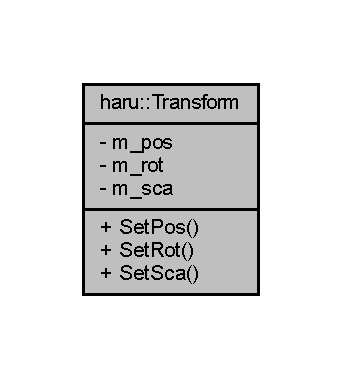
\includegraphics[width=164pt]{classharu_1_1_transform__coll__graph}
\end{center}
\end{figure}
\subsection*{Public Member Functions}
\begin{DoxyCompactItemize}
\item 
void \mbox{\hyperlink{classharu_1_1_transform_a6fd0db91da93d5e88ae6c71559563823}{Set\+Pos}} (glm\+::vec3 \+\_\+pos)
\item 
void \mbox{\hyperlink{classharu_1_1_transform_a8c27baa1c0c35b0a9bd8e1e60f158262}{Set\+Rot}} (glm\+::vec3 \+\_\+rot)
\item 
void \mbox{\hyperlink{classharu_1_1_transform_a16f09008ba3b2effca7f1004caa61ef3}{Set\+Sca}} (glm\+::vec3 \+\_\+sca)
\end{DoxyCompactItemize}
\subsection*{Private Attributes}
\begin{DoxyCompactItemize}
\item 
glm\+::vec3 \mbox{\hyperlink{classharu_1_1_transform_a35eaba7475c13b6ad5925d112e4970ac}{m\+\_\+pos}}
\item 
glm\+::vec3 \mbox{\hyperlink{classharu_1_1_transform_af4ed94d05315ca5235e8a7ee7dd11990}{m\+\_\+rot}}
\item 
glm\+::vec3 \mbox{\hyperlink{classharu_1_1_transform_a1bba1e129d40a560ac0615b8e2de0d6e}{m\+\_\+sca}}
\end{DoxyCompactItemize}


\subsection{Member Function Documentation}
\mbox{\Hypertarget{classharu_1_1_transform_a6fd0db91da93d5e88ae6c71559563823}\label{classharu_1_1_transform_a6fd0db91da93d5e88ae6c71559563823}} 
\index{haru\+::\+Transform@{haru\+::\+Transform}!Set\+Pos@{Set\+Pos}}
\index{Set\+Pos@{Set\+Pos}!haru\+::\+Transform@{haru\+::\+Transform}}
\subsubsection{\texorpdfstring{Set\+Pos()}{SetPos()}}
{\footnotesize\ttfamily void haru\+::\+Transform\+::\+Set\+Pos (\begin{DoxyParamCaption}\item[{glm\+::vec3}]{\+\_\+pos }\end{DoxyParamCaption})}

\mbox{\Hypertarget{classharu_1_1_transform_a8c27baa1c0c35b0a9bd8e1e60f158262}\label{classharu_1_1_transform_a8c27baa1c0c35b0a9bd8e1e60f158262}} 
\index{haru\+::\+Transform@{haru\+::\+Transform}!Set\+Rot@{Set\+Rot}}
\index{Set\+Rot@{Set\+Rot}!haru\+::\+Transform@{haru\+::\+Transform}}
\subsubsection{\texorpdfstring{Set\+Rot()}{SetRot()}}
{\footnotesize\ttfamily void haru\+::\+Transform\+::\+Set\+Rot (\begin{DoxyParamCaption}\item[{glm\+::vec3}]{\+\_\+rot }\end{DoxyParamCaption})}

\mbox{\Hypertarget{classharu_1_1_transform_a16f09008ba3b2effca7f1004caa61ef3}\label{classharu_1_1_transform_a16f09008ba3b2effca7f1004caa61ef3}} 
\index{haru\+::\+Transform@{haru\+::\+Transform}!Set\+Sca@{Set\+Sca}}
\index{Set\+Sca@{Set\+Sca}!haru\+::\+Transform@{haru\+::\+Transform}}
\subsubsection{\texorpdfstring{Set\+Sca()}{SetSca()}}
{\footnotesize\ttfamily void haru\+::\+Transform\+::\+Set\+Sca (\begin{DoxyParamCaption}\item[{glm\+::vec3}]{\+\_\+sca }\end{DoxyParamCaption})}



\subsection{Member Data Documentation}
\mbox{\Hypertarget{classharu_1_1_transform_a35eaba7475c13b6ad5925d112e4970ac}\label{classharu_1_1_transform_a35eaba7475c13b6ad5925d112e4970ac}} 
\index{haru\+::\+Transform@{haru\+::\+Transform}!m\+\_\+pos@{m\+\_\+pos}}
\index{m\+\_\+pos@{m\+\_\+pos}!haru\+::\+Transform@{haru\+::\+Transform}}
\subsubsection{\texorpdfstring{m\+\_\+pos}{m\_pos}}
{\footnotesize\ttfamily glm\+::vec3 haru\+::\+Transform\+::m\+\_\+pos\hspace{0.3cm}{\ttfamily [private]}}

\mbox{\Hypertarget{classharu_1_1_transform_af4ed94d05315ca5235e8a7ee7dd11990}\label{classharu_1_1_transform_af4ed94d05315ca5235e8a7ee7dd11990}} 
\index{haru\+::\+Transform@{haru\+::\+Transform}!m\+\_\+rot@{m\+\_\+rot}}
\index{m\+\_\+rot@{m\+\_\+rot}!haru\+::\+Transform@{haru\+::\+Transform}}
\subsubsection{\texorpdfstring{m\+\_\+rot}{m\_rot}}
{\footnotesize\ttfamily glm\+::vec3 haru\+::\+Transform\+::m\+\_\+rot\hspace{0.3cm}{\ttfamily [private]}}

\mbox{\Hypertarget{classharu_1_1_transform_a1bba1e129d40a560ac0615b8e2de0d6e}\label{classharu_1_1_transform_a1bba1e129d40a560ac0615b8e2de0d6e}} 
\index{haru\+::\+Transform@{haru\+::\+Transform}!m\+\_\+sca@{m\+\_\+sca}}
\index{m\+\_\+sca@{m\+\_\+sca}!haru\+::\+Transform@{haru\+::\+Transform}}
\subsubsection{\texorpdfstring{m\+\_\+sca}{m\_sca}}
{\footnotesize\ttfamily glm\+::vec3 haru\+::\+Transform\+::m\+\_\+sca\hspace{0.3cm}{\ttfamily [private]}}



The documentation for this class was generated from the following files\+:\begin{DoxyCompactItemize}
\item 
source/haruengine/\mbox{\hyperlink{_transform_8h}{Transform.\+h}}\item 
source/haruengine/\mbox{\hyperlink{_transform_8cpp}{Transform.\+cpp}}\end{DoxyCompactItemize}

\hypertarget{classharu_1_1_vertex_array}{}\section{haru\+:\+:Vertex\+Array Class Reference}
\label{classharu_1_1_vertex_array}\index{haru\+::\+Vertex\+Array@{haru\+::\+Vertex\+Array}}


{\ttfamily \#include $<$Vertex\+Array.\+h$>$}



Collaboration diagram for haru\+:\+:Vertex\+Array\+:\nopagebreak
\begin{figure}[H]
\begin{center}
\leavevmode
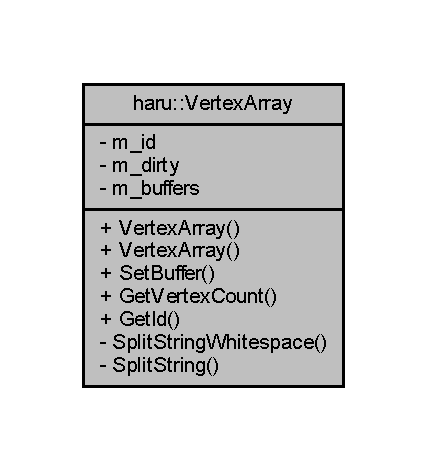
\includegraphics[width=205pt]{classharu_1_1_vertex_array__coll__graph}
\end{center}
\end{figure}
\subsection*{Public Member Functions}
\begin{DoxyCompactItemize}
\item 
\mbox{\hyperlink{classharu_1_1_vertex_array_a53d1c5c6eb05c265f05ed9d06d748f02}{Vertex\+Array}} ()
\item 
\mbox{\hyperlink{classharu_1_1_vertex_array_a8d90e298064690ca3e0ad7fc9aec81b6}{Vertex\+Array}} (std\+::string \+\_\+path)
\item 
void \mbox{\hyperlink{classharu_1_1_vertex_array_aef555fb0ec34f06ed93b9f0d489bf188}{Set\+Buffer}} (std\+::string \+\_\+attribute, std\+::shared\+\_\+ptr$<$ \mbox{\hyperlink{classharu_1_1_vertex_buffer}{Vertex\+Buffer}} $>$ \+\_\+buffer)
\item 
int \mbox{\hyperlink{classharu_1_1_vertex_array_af444883400ad80eacbc8bf32d40a51e1}{Get\+Vertex\+Count}} ()
\item 
G\+Luint \mbox{\hyperlink{classharu_1_1_vertex_array_a9e0954bbf40bfd23997bd4a396e037c0}{Get\+Id}} ()
\end{DoxyCompactItemize}
\subsection*{Private Member Functions}
\begin{DoxyCompactItemize}
\item 
void \mbox{\hyperlink{classharu_1_1_vertex_array_a4881c24fdca7f802456d1b8823a0c4ce}{Split\+String\+Whitespace}} (std\+::string \&\+\_\+input, std\+::vector$<$ std\+::string $>$ \&\+\_\+output)
\item 
void \mbox{\hyperlink{classharu_1_1_vertex_array_a8ca455fffbc9f554851fe18eb8a26bfa}{Split\+String}} (std\+::string \&\+\_\+input, char \+\_\+splitter, std\+::vector$<$ std\+::string $>$ \&\+\_\+output)
\end{DoxyCompactItemize}
\subsection*{Private Attributes}
\begin{DoxyCompactItemize}
\item 
G\+Luint \mbox{\hyperlink{classharu_1_1_vertex_array_a61e6c2025f2bb9da20280c6b607e4c22}{m\+\_\+id}}
\item 
bool \mbox{\hyperlink{classharu_1_1_vertex_array_a7cc151adcf4133de6d7130e206e08b9d}{m\+\_\+dirty}}
\item 
std\+::vector$<$ std\+::shared\+\_\+ptr$<$ \mbox{\hyperlink{classharu_1_1_vertex_buffer}{Vertex\+Buffer}} $>$ $>$ \mbox{\hyperlink{classharu_1_1_vertex_array_a66f9492ccad01a67ed2dff56feefef46}{m\+\_\+buffers}}
\end{DoxyCompactItemize}


\subsection{Constructor \& Destructor Documentation}
\mbox{\Hypertarget{classharu_1_1_vertex_array_a53d1c5c6eb05c265f05ed9d06d748f02}\label{classharu_1_1_vertex_array_a53d1c5c6eb05c265f05ed9d06d748f02}} 
\index{haru\+::\+Vertex\+Array@{haru\+::\+Vertex\+Array}!Vertex\+Array@{Vertex\+Array}}
\index{Vertex\+Array@{Vertex\+Array}!haru\+::\+Vertex\+Array@{haru\+::\+Vertex\+Array}}
\subsubsection{\texorpdfstring{Vertex\+Array()}{VertexArray()}\hspace{0.1cm}{\footnotesize\ttfamily [1/2]}}
{\footnotesize\ttfamily haru\+::\+Vertex\+Array\+::\+Vertex\+Array (\begin{DoxyParamCaption}{ }\end{DoxyParamCaption})}

\mbox{\Hypertarget{classharu_1_1_vertex_array_a8d90e298064690ca3e0ad7fc9aec81b6}\label{classharu_1_1_vertex_array_a8d90e298064690ca3e0ad7fc9aec81b6}} 
\index{haru\+::\+Vertex\+Array@{haru\+::\+Vertex\+Array}!Vertex\+Array@{Vertex\+Array}}
\index{Vertex\+Array@{Vertex\+Array}!haru\+::\+Vertex\+Array@{haru\+::\+Vertex\+Array}}
\subsubsection{\texorpdfstring{Vertex\+Array()}{VertexArray()}\hspace{0.1cm}{\footnotesize\ttfamily [2/2]}}
{\footnotesize\ttfamily haru\+::\+Vertex\+Array\+::\+Vertex\+Array (\begin{DoxyParamCaption}\item[{std\+::string}]{\+\_\+path }\end{DoxyParamCaption})}

Here is the call graph for this function\+:
\nopagebreak
\begin{figure}[H]
\begin{center}
\leavevmode
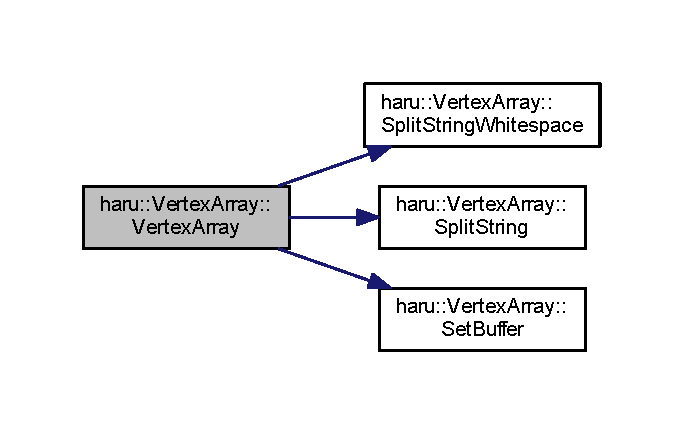
\includegraphics[width=328pt]{classharu_1_1_vertex_array_a8d90e298064690ca3e0ad7fc9aec81b6_cgraph}
\end{center}
\end{figure}


\subsection{Member Function Documentation}
\mbox{\Hypertarget{classharu_1_1_vertex_array_a9e0954bbf40bfd23997bd4a396e037c0}\label{classharu_1_1_vertex_array_a9e0954bbf40bfd23997bd4a396e037c0}} 
\index{haru\+::\+Vertex\+Array@{haru\+::\+Vertex\+Array}!Get\+Id@{Get\+Id}}
\index{Get\+Id@{Get\+Id}!haru\+::\+Vertex\+Array@{haru\+::\+Vertex\+Array}}
\subsubsection{\texorpdfstring{Get\+Id()}{GetId()}}
{\footnotesize\ttfamily G\+Luint haru\+::\+Vertex\+Array\+::\+Get\+Id (\begin{DoxyParamCaption}{ }\end{DoxyParamCaption})}

\mbox{\Hypertarget{classharu_1_1_vertex_array_af444883400ad80eacbc8bf32d40a51e1}\label{classharu_1_1_vertex_array_af444883400ad80eacbc8bf32d40a51e1}} 
\index{haru\+::\+Vertex\+Array@{haru\+::\+Vertex\+Array}!Get\+Vertex\+Count@{Get\+Vertex\+Count}}
\index{Get\+Vertex\+Count@{Get\+Vertex\+Count}!haru\+::\+Vertex\+Array@{haru\+::\+Vertex\+Array}}
\subsubsection{\texorpdfstring{Get\+Vertex\+Count()}{GetVertexCount()}}
{\footnotesize\ttfamily int haru\+::\+Vertex\+Array\+::\+Get\+Vertex\+Count (\begin{DoxyParamCaption}{ }\end{DoxyParamCaption})}

\mbox{\Hypertarget{classharu_1_1_vertex_array_aef555fb0ec34f06ed93b9f0d489bf188}\label{classharu_1_1_vertex_array_aef555fb0ec34f06ed93b9f0d489bf188}} 
\index{haru\+::\+Vertex\+Array@{haru\+::\+Vertex\+Array}!Set\+Buffer@{Set\+Buffer}}
\index{Set\+Buffer@{Set\+Buffer}!haru\+::\+Vertex\+Array@{haru\+::\+Vertex\+Array}}
\subsubsection{\texorpdfstring{Set\+Buffer()}{SetBuffer()}}
{\footnotesize\ttfamily void haru\+::\+Vertex\+Array\+::\+Set\+Buffer (\begin{DoxyParamCaption}\item[{std\+::string}]{\+\_\+attribute,  }\item[{std\+::shared\+\_\+ptr$<$ \mbox{\hyperlink{classharu_1_1_vertex_buffer}{Vertex\+Buffer}} $>$}]{\+\_\+buffer }\end{DoxyParamCaption})}

Here is the caller graph for this function\+:
\nopagebreak
\begin{figure}[H]
\begin{center}
\leavevmode
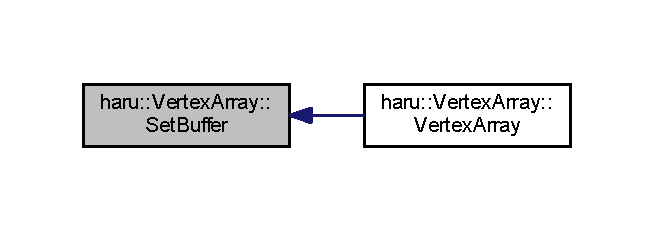
\includegraphics[width=314pt]{classharu_1_1_vertex_array_aef555fb0ec34f06ed93b9f0d489bf188_icgraph}
\end{center}
\end{figure}
\mbox{\Hypertarget{classharu_1_1_vertex_array_a8ca455fffbc9f554851fe18eb8a26bfa}\label{classharu_1_1_vertex_array_a8ca455fffbc9f554851fe18eb8a26bfa}} 
\index{haru\+::\+Vertex\+Array@{haru\+::\+Vertex\+Array}!Split\+String@{Split\+String}}
\index{Split\+String@{Split\+String}!haru\+::\+Vertex\+Array@{haru\+::\+Vertex\+Array}}
\subsubsection{\texorpdfstring{Split\+String()}{SplitString()}}
{\footnotesize\ttfamily void haru\+::\+Vertex\+Array\+::\+Split\+String (\begin{DoxyParamCaption}\item[{std\+::string \&}]{\+\_\+input,  }\item[{char}]{\+\_\+splitter,  }\item[{std\+::vector$<$ std\+::string $>$ \&}]{\+\_\+output }\end{DoxyParamCaption})\hspace{0.3cm}{\ttfamily [private]}}

Here is the caller graph for this function\+:
\nopagebreak
\begin{figure}[H]
\begin{center}
\leavevmode
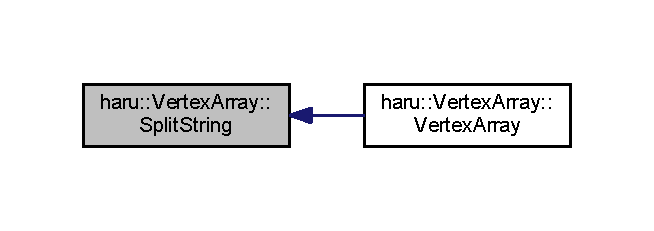
\includegraphics[width=314pt]{classharu_1_1_vertex_array_a8ca455fffbc9f554851fe18eb8a26bfa_icgraph}
\end{center}
\end{figure}
\mbox{\Hypertarget{classharu_1_1_vertex_array_a4881c24fdca7f802456d1b8823a0c4ce}\label{classharu_1_1_vertex_array_a4881c24fdca7f802456d1b8823a0c4ce}} 
\index{haru\+::\+Vertex\+Array@{haru\+::\+Vertex\+Array}!Split\+String\+Whitespace@{Split\+String\+Whitespace}}
\index{Split\+String\+Whitespace@{Split\+String\+Whitespace}!haru\+::\+Vertex\+Array@{haru\+::\+Vertex\+Array}}
\subsubsection{\texorpdfstring{Split\+String\+Whitespace()}{SplitStringWhitespace()}}
{\footnotesize\ttfamily void haru\+::\+Vertex\+Array\+::\+Split\+String\+Whitespace (\begin{DoxyParamCaption}\item[{std\+::string \&}]{\+\_\+input,  }\item[{std\+::vector$<$ std\+::string $>$ \&}]{\+\_\+output }\end{DoxyParamCaption})\hspace{0.3cm}{\ttfamily [private]}}

Here is the caller graph for this function\+:
\nopagebreak
\begin{figure}[H]
\begin{center}
\leavevmode
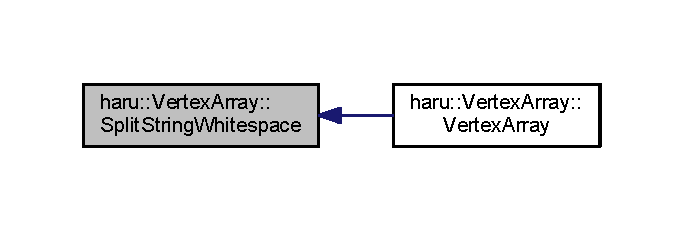
\includegraphics[width=328pt]{classharu_1_1_vertex_array_a4881c24fdca7f802456d1b8823a0c4ce_icgraph}
\end{center}
\end{figure}


\subsection{Member Data Documentation}
\mbox{\Hypertarget{classharu_1_1_vertex_array_a66f9492ccad01a67ed2dff56feefef46}\label{classharu_1_1_vertex_array_a66f9492ccad01a67ed2dff56feefef46}} 
\index{haru\+::\+Vertex\+Array@{haru\+::\+Vertex\+Array}!m\+\_\+buffers@{m\+\_\+buffers}}
\index{m\+\_\+buffers@{m\+\_\+buffers}!haru\+::\+Vertex\+Array@{haru\+::\+Vertex\+Array}}
\subsubsection{\texorpdfstring{m\+\_\+buffers}{m\_buffers}}
{\footnotesize\ttfamily std\+::vector$<$std\+::shared\+\_\+ptr$<$\mbox{\hyperlink{classharu_1_1_vertex_buffer}{Vertex\+Buffer}}$>$ $>$ haru\+::\+Vertex\+Array\+::m\+\_\+buffers\hspace{0.3cm}{\ttfamily [private]}}

\mbox{\Hypertarget{classharu_1_1_vertex_array_a7cc151adcf4133de6d7130e206e08b9d}\label{classharu_1_1_vertex_array_a7cc151adcf4133de6d7130e206e08b9d}} 
\index{haru\+::\+Vertex\+Array@{haru\+::\+Vertex\+Array}!m\+\_\+dirty@{m\+\_\+dirty}}
\index{m\+\_\+dirty@{m\+\_\+dirty}!haru\+::\+Vertex\+Array@{haru\+::\+Vertex\+Array}}
\subsubsection{\texorpdfstring{m\+\_\+dirty}{m\_dirty}}
{\footnotesize\ttfamily bool haru\+::\+Vertex\+Array\+::m\+\_\+dirty\hspace{0.3cm}{\ttfamily [private]}}

\mbox{\Hypertarget{classharu_1_1_vertex_array_a61e6c2025f2bb9da20280c6b607e4c22}\label{classharu_1_1_vertex_array_a61e6c2025f2bb9da20280c6b607e4c22}} 
\index{haru\+::\+Vertex\+Array@{haru\+::\+Vertex\+Array}!m\+\_\+id@{m\+\_\+id}}
\index{m\+\_\+id@{m\+\_\+id}!haru\+::\+Vertex\+Array@{haru\+::\+Vertex\+Array}}
\subsubsection{\texorpdfstring{m\+\_\+id}{m\_id}}
{\footnotesize\ttfamily G\+Luint haru\+::\+Vertex\+Array\+::m\+\_\+id\hspace{0.3cm}{\ttfamily [private]}}



The documentation for this class was generated from the following files\+:\begin{DoxyCompactItemize}
\item 
source/haruengine/\mbox{\hyperlink{_vertex_array_8h}{Vertex\+Array.\+h}}\item 
source/haruengine/\mbox{\hyperlink{_vertex_array_8cpp}{Vertex\+Array.\+cpp}}\end{DoxyCompactItemize}

\hypertarget{classharu_1_1_vertex_buffer}{}\section{haru\+:\+:Vertex\+Buffer Class Reference}
\label{classharu_1_1_vertex_buffer}\index{haru\+::\+Vertex\+Buffer@{haru\+::\+Vertex\+Buffer}}


{\ttfamily \#include $<$Vertex\+Buffer.\+h$>$}



Collaboration diagram for haru\+:\+:Vertex\+Buffer\+:\nopagebreak
\begin{figure}[H]
\begin{center}
\leavevmode
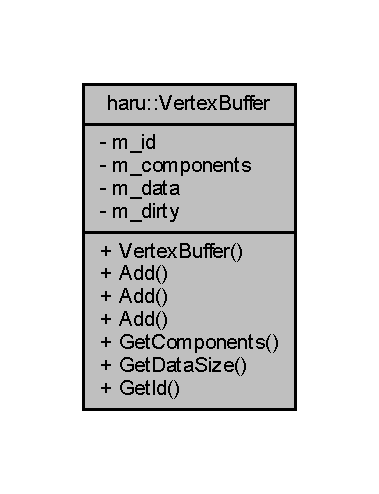
\includegraphics[width=182pt]{classharu_1_1_vertex_buffer__coll__graph}
\end{center}
\end{figure}
\subsection*{Public Member Functions}
\begin{DoxyCompactItemize}
\item 
\mbox{\hyperlink{classharu_1_1_vertex_buffer_a97d2aa926c9d0f52e23687a7f283744f}{Vertex\+Buffer}} ()
\item 
void \mbox{\hyperlink{classharu_1_1_vertex_buffer_a5342e907f32b100831c4380086ecbd32}{Add}} (glm\+::vec2 \+\_\+value)
\item 
void \mbox{\hyperlink{classharu_1_1_vertex_buffer_a1494c4813a370bc9cefa125d1f6ecfda}{Add}} (glm\+::vec3 \+\_\+value)
\item 
void \mbox{\hyperlink{classharu_1_1_vertex_buffer_a6f121147bd44ce3c9a8487a3c9650262}{Add}} (glm\+::vec4 \+\_\+value)
\item 
int \mbox{\hyperlink{classharu_1_1_vertex_buffer_a8f98140e1a99aa3490189914d1498031}{Get\+Components}} ()
\item 
int \mbox{\hyperlink{classharu_1_1_vertex_buffer_aa5e656255932e3be2d53ba4ab1165667}{Get\+Data\+Size}} ()
\item 
G\+Luint \mbox{\hyperlink{classharu_1_1_vertex_buffer_a9cf4caf3c2221d4229d1d263979ac74a}{Get\+Id}} ()
\end{DoxyCompactItemize}
\subsection*{Private Attributes}
\begin{DoxyCompactItemize}
\item 
G\+Luint \mbox{\hyperlink{classharu_1_1_vertex_buffer_a63aad09771ce7a6722d56e56c0e09922}{m\+\_\+id}}
\item 
int \mbox{\hyperlink{classharu_1_1_vertex_buffer_ab606ca1fca949eb662749ac4986fc638}{m\+\_\+components}}
\item 
std\+::vector$<$ G\+Lfloat $>$ \mbox{\hyperlink{classharu_1_1_vertex_buffer_a0e1dd6e128d66ccb719c7efec8afcc19}{m\+\_\+data}}
\item 
bool \mbox{\hyperlink{classharu_1_1_vertex_buffer_a42cc7fd939921990cad71e1e3856725c}{m\+\_\+dirty}}
\end{DoxyCompactItemize}


\subsection{Constructor \& Destructor Documentation}
\mbox{\Hypertarget{classharu_1_1_vertex_buffer_a97d2aa926c9d0f52e23687a7f283744f}\label{classharu_1_1_vertex_buffer_a97d2aa926c9d0f52e23687a7f283744f}} 
\index{haru\+::\+Vertex\+Buffer@{haru\+::\+Vertex\+Buffer}!Vertex\+Buffer@{Vertex\+Buffer}}
\index{Vertex\+Buffer@{Vertex\+Buffer}!haru\+::\+Vertex\+Buffer@{haru\+::\+Vertex\+Buffer}}
\subsubsection{\texorpdfstring{Vertex\+Buffer()}{VertexBuffer()}}
{\footnotesize\ttfamily haru\+::\+Vertex\+Buffer\+::\+Vertex\+Buffer (\begin{DoxyParamCaption}{ }\end{DoxyParamCaption})}



\subsection{Member Function Documentation}
\mbox{\Hypertarget{classharu_1_1_vertex_buffer_a5342e907f32b100831c4380086ecbd32}\label{classharu_1_1_vertex_buffer_a5342e907f32b100831c4380086ecbd32}} 
\index{haru\+::\+Vertex\+Buffer@{haru\+::\+Vertex\+Buffer}!Add@{Add}}
\index{Add@{Add}!haru\+::\+Vertex\+Buffer@{haru\+::\+Vertex\+Buffer}}
\subsubsection{\texorpdfstring{Add()}{Add()}\hspace{0.1cm}{\footnotesize\ttfamily [1/3]}}
{\footnotesize\ttfamily void haru\+::\+Vertex\+Buffer\+::\+Add (\begin{DoxyParamCaption}\item[{glm\+::vec2}]{\+\_\+value }\end{DoxyParamCaption})}

\mbox{\Hypertarget{classharu_1_1_vertex_buffer_a1494c4813a370bc9cefa125d1f6ecfda}\label{classharu_1_1_vertex_buffer_a1494c4813a370bc9cefa125d1f6ecfda}} 
\index{haru\+::\+Vertex\+Buffer@{haru\+::\+Vertex\+Buffer}!Add@{Add}}
\index{Add@{Add}!haru\+::\+Vertex\+Buffer@{haru\+::\+Vertex\+Buffer}}
\subsubsection{\texorpdfstring{Add()}{Add()}\hspace{0.1cm}{\footnotesize\ttfamily [2/3]}}
{\footnotesize\ttfamily void haru\+::\+Vertex\+Buffer\+::\+Add (\begin{DoxyParamCaption}\item[{glm\+::vec3}]{\+\_\+value }\end{DoxyParamCaption})}

\mbox{\Hypertarget{classharu_1_1_vertex_buffer_a6f121147bd44ce3c9a8487a3c9650262}\label{classharu_1_1_vertex_buffer_a6f121147bd44ce3c9a8487a3c9650262}} 
\index{haru\+::\+Vertex\+Buffer@{haru\+::\+Vertex\+Buffer}!Add@{Add}}
\index{Add@{Add}!haru\+::\+Vertex\+Buffer@{haru\+::\+Vertex\+Buffer}}
\subsubsection{\texorpdfstring{Add()}{Add()}\hspace{0.1cm}{\footnotesize\ttfamily [3/3]}}
{\footnotesize\ttfamily void haru\+::\+Vertex\+Buffer\+::\+Add (\begin{DoxyParamCaption}\item[{glm\+::vec4}]{\+\_\+value }\end{DoxyParamCaption})}

\mbox{\Hypertarget{classharu_1_1_vertex_buffer_a8f98140e1a99aa3490189914d1498031}\label{classharu_1_1_vertex_buffer_a8f98140e1a99aa3490189914d1498031}} 
\index{haru\+::\+Vertex\+Buffer@{haru\+::\+Vertex\+Buffer}!Get\+Components@{Get\+Components}}
\index{Get\+Components@{Get\+Components}!haru\+::\+Vertex\+Buffer@{haru\+::\+Vertex\+Buffer}}
\subsubsection{\texorpdfstring{Get\+Components()}{GetComponents()}}
{\footnotesize\ttfamily int haru\+::\+Vertex\+Buffer\+::\+Get\+Components (\begin{DoxyParamCaption}{ }\end{DoxyParamCaption})}

\mbox{\Hypertarget{classharu_1_1_vertex_buffer_aa5e656255932e3be2d53ba4ab1165667}\label{classharu_1_1_vertex_buffer_aa5e656255932e3be2d53ba4ab1165667}} 
\index{haru\+::\+Vertex\+Buffer@{haru\+::\+Vertex\+Buffer}!Get\+Data\+Size@{Get\+Data\+Size}}
\index{Get\+Data\+Size@{Get\+Data\+Size}!haru\+::\+Vertex\+Buffer@{haru\+::\+Vertex\+Buffer}}
\subsubsection{\texorpdfstring{Get\+Data\+Size()}{GetDataSize()}}
{\footnotesize\ttfamily int haru\+::\+Vertex\+Buffer\+::\+Get\+Data\+Size (\begin{DoxyParamCaption}{ }\end{DoxyParamCaption})}

\mbox{\Hypertarget{classharu_1_1_vertex_buffer_a9cf4caf3c2221d4229d1d263979ac74a}\label{classharu_1_1_vertex_buffer_a9cf4caf3c2221d4229d1d263979ac74a}} 
\index{haru\+::\+Vertex\+Buffer@{haru\+::\+Vertex\+Buffer}!Get\+Id@{Get\+Id}}
\index{Get\+Id@{Get\+Id}!haru\+::\+Vertex\+Buffer@{haru\+::\+Vertex\+Buffer}}
\subsubsection{\texorpdfstring{Get\+Id()}{GetId()}}
{\footnotesize\ttfamily G\+Luint haru\+::\+Vertex\+Buffer\+::\+Get\+Id (\begin{DoxyParamCaption}{ }\end{DoxyParamCaption})}



\subsection{Member Data Documentation}
\mbox{\Hypertarget{classharu_1_1_vertex_buffer_ab606ca1fca949eb662749ac4986fc638}\label{classharu_1_1_vertex_buffer_ab606ca1fca949eb662749ac4986fc638}} 
\index{haru\+::\+Vertex\+Buffer@{haru\+::\+Vertex\+Buffer}!m\+\_\+components@{m\+\_\+components}}
\index{m\+\_\+components@{m\+\_\+components}!haru\+::\+Vertex\+Buffer@{haru\+::\+Vertex\+Buffer}}
\subsubsection{\texorpdfstring{m\+\_\+components}{m\_components}}
{\footnotesize\ttfamily int haru\+::\+Vertex\+Buffer\+::m\+\_\+components\hspace{0.3cm}{\ttfamily [private]}}

\mbox{\Hypertarget{classharu_1_1_vertex_buffer_a0e1dd6e128d66ccb719c7efec8afcc19}\label{classharu_1_1_vertex_buffer_a0e1dd6e128d66ccb719c7efec8afcc19}} 
\index{haru\+::\+Vertex\+Buffer@{haru\+::\+Vertex\+Buffer}!m\+\_\+data@{m\+\_\+data}}
\index{m\+\_\+data@{m\+\_\+data}!haru\+::\+Vertex\+Buffer@{haru\+::\+Vertex\+Buffer}}
\subsubsection{\texorpdfstring{m\+\_\+data}{m\_data}}
{\footnotesize\ttfamily std\+::vector$<$G\+Lfloat$>$ haru\+::\+Vertex\+Buffer\+::m\+\_\+data\hspace{0.3cm}{\ttfamily [private]}}

\mbox{\Hypertarget{classharu_1_1_vertex_buffer_a42cc7fd939921990cad71e1e3856725c}\label{classharu_1_1_vertex_buffer_a42cc7fd939921990cad71e1e3856725c}} 
\index{haru\+::\+Vertex\+Buffer@{haru\+::\+Vertex\+Buffer}!m\+\_\+dirty@{m\+\_\+dirty}}
\index{m\+\_\+dirty@{m\+\_\+dirty}!haru\+::\+Vertex\+Buffer@{haru\+::\+Vertex\+Buffer}}
\subsubsection{\texorpdfstring{m\+\_\+dirty}{m\_dirty}}
{\footnotesize\ttfamily bool haru\+::\+Vertex\+Buffer\+::m\+\_\+dirty\hspace{0.3cm}{\ttfamily [private]}}

\mbox{\Hypertarget{classharu_1_1_vertex_buffer_a63aad09771ce7a6722d56e56c0e09922}\label{classharu_1_1_vertex_buffer_a63aad09771ce7a6722d56e56c0e09922}} 
\index{haru\+::\+Vertex\+Buffer@{haru\+::\+Vertex\+Buffer}!m\+\_\+id@{m\+\_\+id}}
\index{m\+\_\+id@{m\+\_\+id}!haru\+::\+Vertex\+Buffer@{haru\+::\+Vertex\+Buffer}}
\subsubsection{\texorpdfstring{m\+\_\+id}{m\_id}}
{\footnotesize\ttfamily G\+Luint haru\+::\+Vertex\+Buffer\+::m\+\_\+id\hspace{0.3cm}{\ttfamily [private]}}



The documentation for this class was generated from the following files\+:\begin{DoxyCompactItemize}
\item 
source/haruengine/\mbox{\hyperlink{_vertex_buffer_8h}{Vertex\+Buffer.\+h}}\item 
source/haruengine/\mbox{\hyperlink{_vertex_buffer_8cpp}{Vertex\+Buffer.\+cpp}}\end{DoxyCompactItemize}

\chapter{File Documentation}
\hypertarget{main_8cpp}{}\section{source/game/main.cpp File Reference}
\label{main_8cpp}\index{source/game/main.\+cpp@{source/game/main.\+cpp}}
{\ttfamily \#include $<$haruengine/haru.\+h$>$}\newline
{\ttfamily \#include $<$iostream$>$}\newline
Include dependency graph for main.\+cpp\+:\nopagebreak
\begin{figure}[H]
\begin{center}
\leavevmode
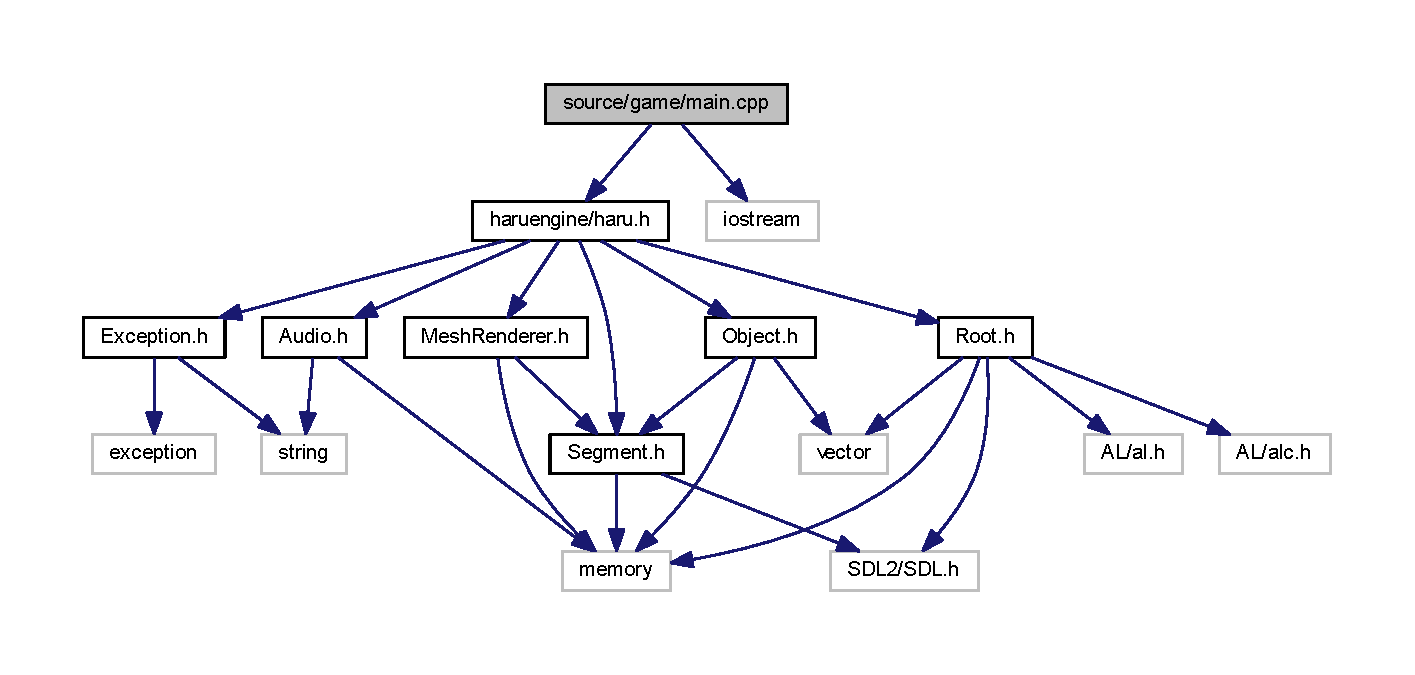
\includegraphics[width=350pt]{main_8cpp__incl}
\end{center}
\end{figure}
\subsection*{Functions}
\begin{DoxyCompactItemize}
\item 
int \mbox{\hyperlink{main_8cpp_ae66f6b31b5ad750f1fe042a706a4e3d4}{main}} ()
\end{DoxyCompactItemize}


\subsection{Function Documentation}
\mbox{\Hypertarget{main_8cpp_ae66f6b31b5ad750f1fe042a706a4e3d4}\label{main_8cpp_ae66f6b31b5ad750f1fe042a706a4e3d4}} 
\index{main.\+cpp@{main.\+cpp}!main@{main}}
\index{main@{main}!main.\+cpp@{main.\+cpp}}
\subsubsection{\texorpdfstring{main()}{main()}}
{\footnotesize\ttfamily int main (\begin{DoxyParamCaption}{ }\end{DoxyParamCaption})}

Here is the call graph for this function\+:\nopagebreak
\begin{figure}[H]
\begin{center}
\leavevmode
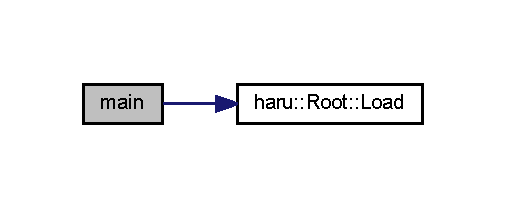
\includegraphics[width=243pt]{main_8cpp_ae66f6b31b5ad750f1fe042a706a4e3d4_cgraph}
\end{center}
\end{figure}

\hypertarget{_audio_8cpp}{}\section{source/haruengine/\+Audio.cpp File Reference}
\label{_audio_8cpp}\index{source/haruengine/\+Audio.\+cpp@{source/haruengine/\+Audio.\+cpp}}
{\ttfamily \#include \char`\"{}Audio.\+h\char`\"{}}\newline
{\ttfamily \#include $<$A\+L/al.\+h$>$}\newline
{\ttfamily \#include $<$vorbis/vorbisfile.\+h$>$}\newline
{\ttfamily \#include $<$iostream$>$}\newline
{\ttfamily \#include $<$vector$>$}\newline
Include dependency graph for Audio.\+cpp\+:\nopagebreak
\begin{figure}[H]
\begin{center}
\leavevmode
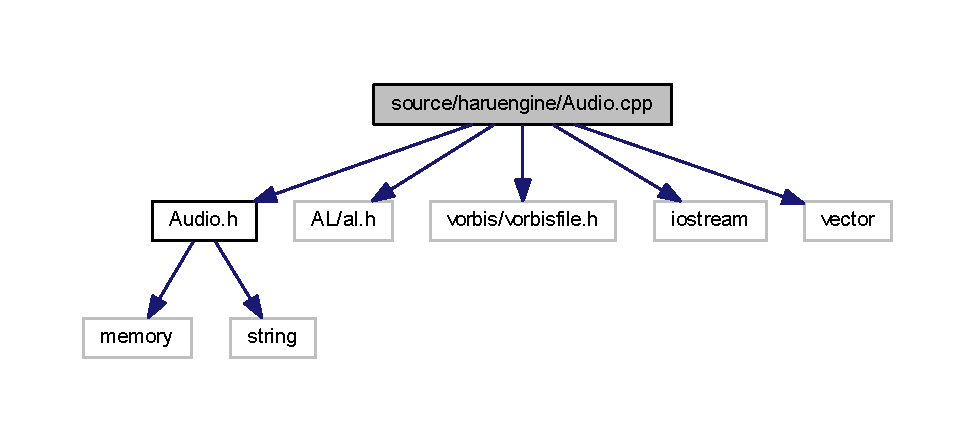
\includegraphics[width=350pt]{_audio_8cpp__incl}
\end{center}
\end{figure}
\subsection*{Classes}
\begin{DoxyCompactItemize}
\item 
struct \mbox{\hyperlink{structharu_1_1_audio_impl}{haru\+::\+Audio\+Impl}}
\end{DoxyCompactItemize}
\subsection*{Namespaces}
\begin{DoxyCompactItemize}
\item 
 \mbox{\hyperlink{namespaceharu}{haru}}
\end{DoxyCompactItemize}

\hypertarget{_audio_8h}{}\section{source/haruengine/\+Audio.h File Reference}
\label{_audio_8h}\index{source/haruengine/\+Audio.\+h@{source/haruengine/\+Audio.\+h}}
{\ttfamily \#include $<$memory$>$}\newline
{\ttfamily \#include $<$string$>$}\newline
Include dependency graph for Audio.\+h\+:\nopagebreak
\begin{figure}[H]
\begin{center}
\leavevmode
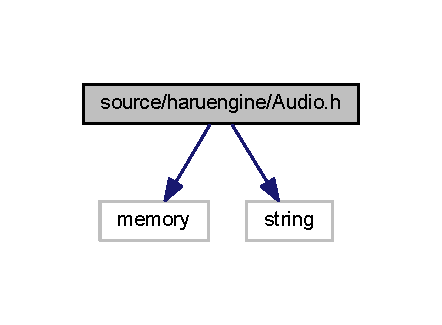
\includegraphics[width=212pt]{_audio_8h__incl}
\end{center}
\end{figure}
This graph shows which files directly or indirectly include this file\+:\nopagebreak
\begin{figure}[H]
\begin{center}
\leavevmode
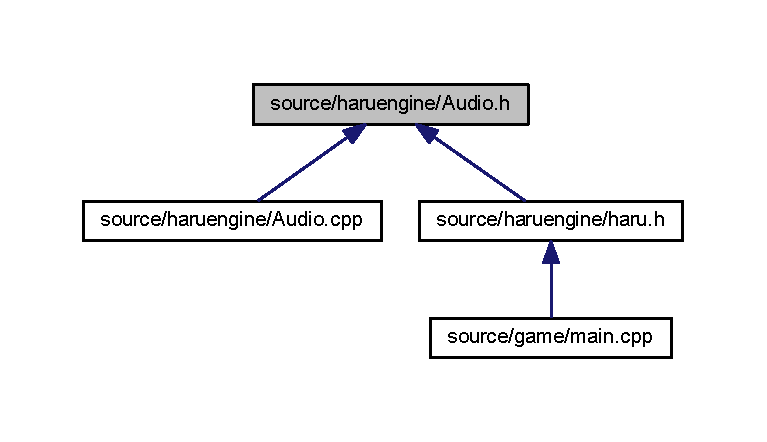
\includegraphics[width=350pt]{_audio_8h__dep__incl}
\end{center}
\end{figure}
\subsection*{Classes}
\begin{DoxyCompactItemize}
\item 
class \mbox{\hyperlink{classharu_1_1_audio}{haru\+::\+Audio}}
\end{DoxyCompactItemize}
\subsection*{Namespaces}
\begin{DoxyCompactItemize}
\item 
 \mbox{\hyperlink{namespaceharu}{haru}}
\end{DoxyCompactItemize}

\hypertarget{_domain_8cpp}{}\section{source/haruengine/\+Domain.cpp File Reference}
\label{_domain_8cpp}\index{source/haruengine/\+Domain.\+cpp@{source/haruengine/\+Domain.\+cpp}}
{\ttfamily \#include \char`\"{}Domain.\+h\char`\"{}}\newline
Include dependency graph for Domain.\+cpp\+:\nopagebreak
\begin{figure}[H]
\begin{center}
\leavevmode
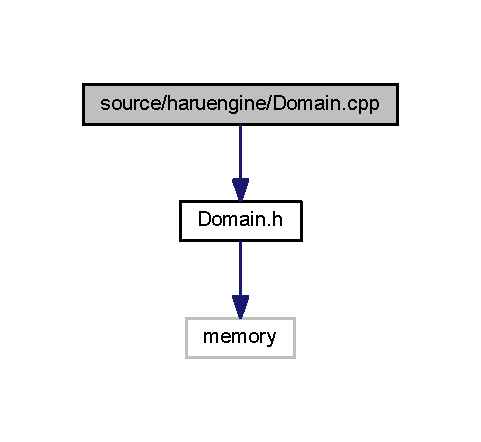
\includegraphics[width=231pt]{_domain_8cpp__incl}
\end{center}
\end{figure}

\hypertarget{_domain_8h}{}\section{source/haruengine/\+Domain.h File Reference}
\label{_domain_8h}\index{source/haruengine/\+Domain.\+h@{source/haruengine/\+Domain.\+h}}
{\ttfamily \#include $<$memory$>$}\newline
Include dependency graph for Domain.\+h\+:\nopagebreak
\begin{figure}[H]
\begin{center}
\leavevmode
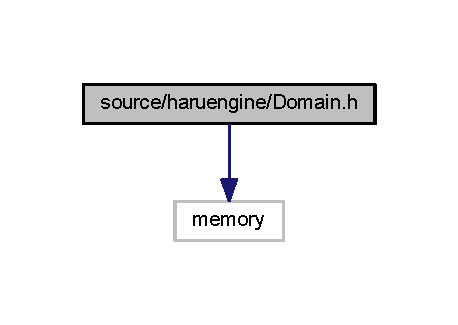
\includegraphics[width=220pt]{_domain_8h__incl}
\end{center}
\end{figure}
This graph shows which files directly or indirectly include this file\+:\nopagebreak
\begin{figure}[H]
\begin{center}
\leavevmode
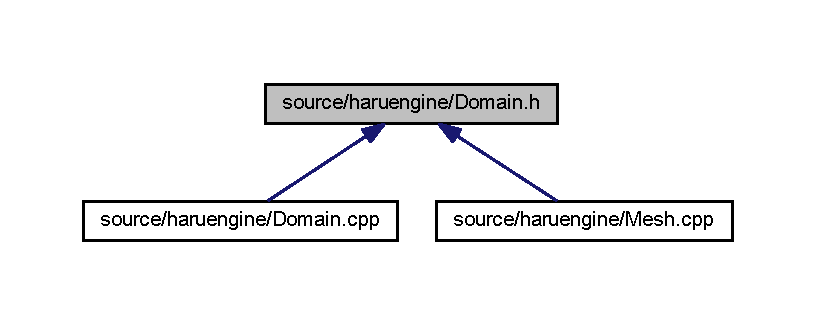
\includegraphics[width=350pt]{_domain_8h__dep__incl}
\end{center}
\end{figure}
\subsection*{Classes}
\begin{DoxyCompactItemize}
\item 
class \mbox{\hyperlink{class_domain}{Domain}}
\end{DoxyCompactItemize}

\hypertarget{_e_screen_8cpp}{}\section{source/haruengine/\+E\+Screen.cpp File Reference}
\label{_e_screen_8cpp}\index{source/haruengine/\+E\+Screen.\+cpp@{source/haruengine/\+E\+Screen.\+cpp}}
{\ttfamily \#include \char`\"{}E\+Screen.\+h\char`\"{}}\newline
Include dependency graph for E\+Screen.\+cpp\+:\nopagebreak
\begin{figure}[H]
\begin{center}
\leavevmode
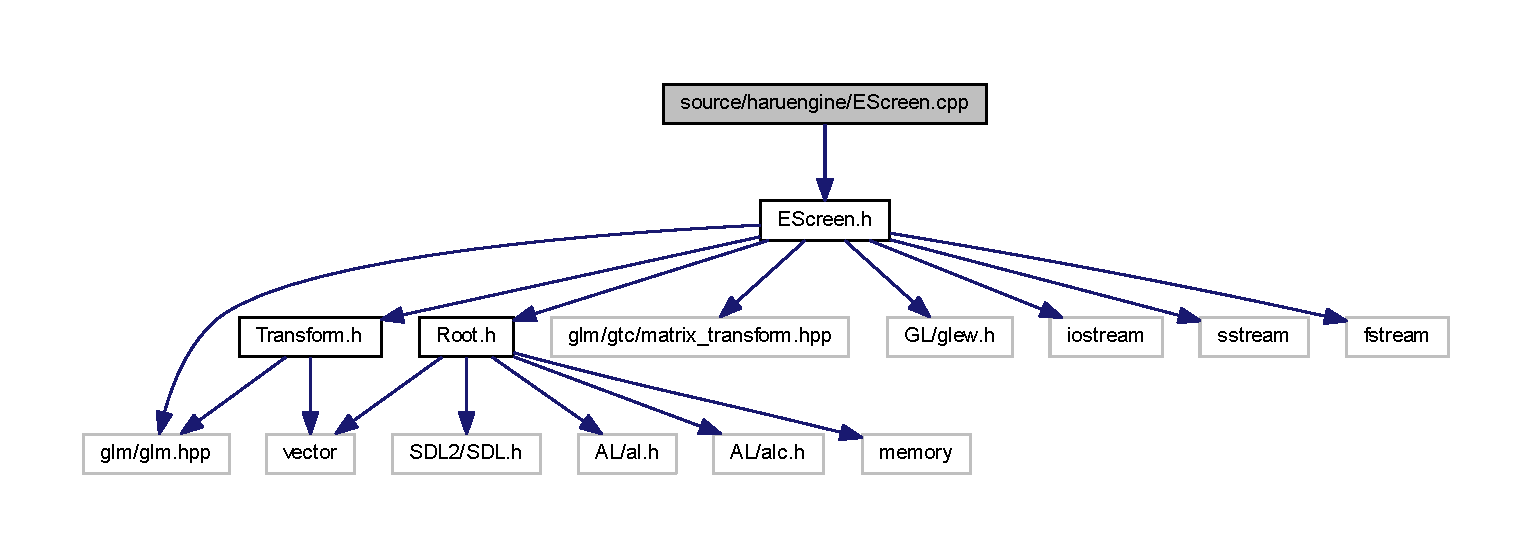
\includegraphics[width=350pt]{_e_screen_8cpp__incl}
\end{center}
\end{figure}
\subsection*{Namespaces}
\begin{DoxyCompactItemize}
\item 
 \mbox{\hyperlink{namespaceharu}{haru}}
\end{DoxyCompactItemize}

\hypertarget{_e_screen_8h}{}\section{source/haruengine/\+E\+Screen.h File Reference}
\label{_e_screen_8h}\index{source/haruengine/\+E\+Screen.\+h@{source/haruengine/\+E\+Screen.\+h}}
{\ttfamily \#include \char`\"{}Transform.\+h\char`\"{}}\newline
{\ttfamily \#include \char`\"{}Root.\+h\char`\"{}}\newline
{\ttfamily \#include $<$glm/glm.\+hpp$>$}\newline
{\ttfamily \#include $<$glm/gtc/matrix\+\_\+transform.\+hpp$>$}\newline
{\ttfamily \#include $<$G\+L/glew.\+h$>$}\newline
{\ttfamily \#include $<$iostream$>$}\newline
{\ttfamily \#include $<$sstream$>$}\newline
{\ttfamily \#include $<$fstream$>$}\newline
Include dependency graph for E\+Screen.\+h\+:\nopagebreak
\begin{figure}[H]
\begin{center}
\leavevmode
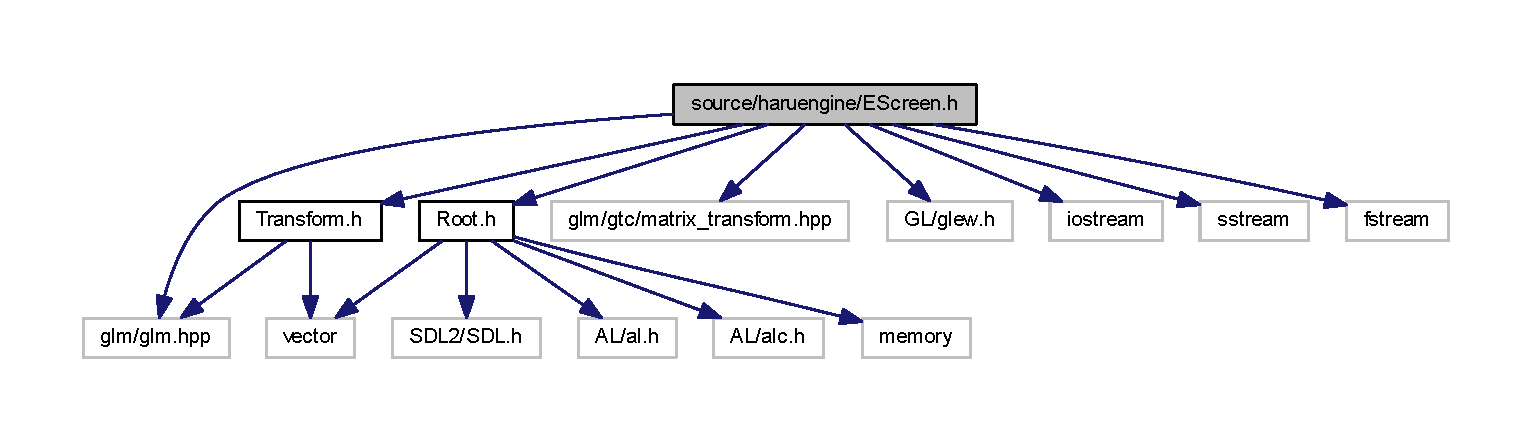
\includegraphics[width=350pt]{_e_screen_8h__incl}
\end{center}
\end{figure}
This graph shows which files directly or indirectly include this file\+:\nopagebreak
\begin{figure}[H]
\begin{center}
\leavevmode
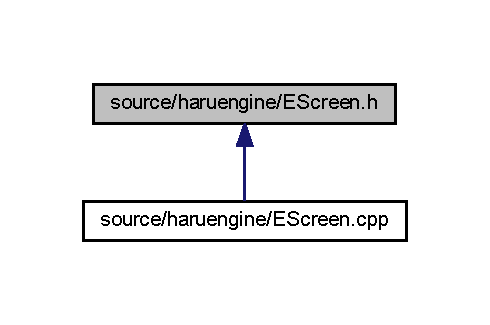
\includegraphics[width=235pt]{_e_screen_8h__dep__incl}
\end{center}
\end{figure}
\subsection*{Classes}
\begin{DoxyCompactItemize}
\item 
class \mbox{\hyperlink{classharu_1_1_e_screen}{haru\+::\+E\+Screen}}
\end{DoxyCompactItemize}
\subsection*{Namespaces}
\begin{DoxyCompactItemize}
\item 
 \mbox{\hyperlink{namespaceharu}{haru}}
\end{DoxyCompactItemize}

\hypertarget{_exception_8cpp}{}\section{source/haruengine/\+Exception.cpp File Reference}
\label{_exception_8cpp}\index{source/haruengine/\+Exception.\+cpp@{source/haruengine/\+Exception.\+cpp}}
{\ttfamily \#include \char`\"{}Exception.\+h\char`\"{}}\newline
{\ttfamily \#include $<$iostream$>$}\newline
Include dependency graph for Exception.\+cpp\+:\nopagebreak
\begin{figure}[H]
\begin{center}
\leavevmode
\includegraphics[width=263pt]{_exception_8cpp__incl}
\end{center}
\end{figure}
\subsection*{Namespaces}
\begin{DoxyCompactItemize}
\item 
 \mbox{\hyperlink{namespaceharu}{haru}}
\end{DoxyCompactItemize}

\hypertarget{_exception_8h}{}\section{source/haruengine/\+Exception.h File Reference}
\label{_exception_8h}\index{source/haruengine/\+Exception.\+h@{source/haruengine/\+Exception.\+h}}
{\ttfamily \#include $<$exception$>$}\newline
{\ttfamily \#include $<$string$>$}\newline
Include dependency graph for Exception.\+h\+:\nopagebreak
\begin{figure}[H]
\begin{center}
\leavevmode
\includegraphics[width=231pt]{_exception_8h__incl}
\end{center}
\end{figure}
This graph shows which files directly or indirectly include this file\+:\nopagebreak
\begin{figure}[H]
\begin{center}
\leavevmode
\includegraphics[width=350pt]{_exception_8h__dep__incl}
\end{center}
\end{figure}
\subsection*{Classes}
\begin{DoxyCompactItemize}
\item 
class \mbox{\hyperlink{classharu_1_1_exception}{haru\+::\+Exception}}
\end{DoxyCompactItemize}
\subsection*{Namespaces}
\begin{DoxyCompactItemize}
\item 
 \mbox{\hyperlink{namespaceharu}{haru}}
\end{DoxyCompactItemize}

\hypertarget{_game_manager_8cpp}{}\section{source/haruengine/\+Game\+Manager.cpp File Reference}
\label{_game_manager_8cpp}\index{source/haruengine/\+Game\+Manager.\+cpp@{source/haruengine/\+Game\+Manager.\+cpp}}
{\ttfamily \#include \char`\"{}Game\+Manager.\+h\char`\"{}}\newline
Include dependency graph for Game\+Manager.\+cpp\+:\nopagebreak
\begin{figure}[H]
\begin{center}
\leavevmode
\includegraphics[width=350pt]{_game_manager_8cpp__incl}
\end{center}
\end{figure}
\subsection*{Namespaces}
\begin{DoxyCompactItemize}
\item 
 \mbox{\hyperlink{namespaceharu}{haru}}
\end{DoxyCompactItemize}

\hypertarget{_game_manager_8h}{}\section{source/haruengine/\+Game\+Manager.h File Reference}
\label{_game_manager_8h}\index{source/haruengine/\+Game\+Manager.\+h@{source/haruengine/\+Game\+Manager.\+h}}
{\ttfamily \#include $<$vector$>$}\newline
{\ttfamily \#include $<$iostream$>$}\newline
{\ttfamily \#include $<$memory$>$}\newline
{\ttfamily \#include $<$string$>$}\newline
{\ttfamily \#include $<$S\+D\+L2/\+S\+D\+L.\+h$>$}\newline
{\ttfamily \#include $<$list$>$}\newline
{\ttfamily \#include \char`\"{}Resource.\+h\char`\"{}}\newline
Include dependency graph for Game\+Manager.\+h\+:\nopagebreak
\begin{figure}[H]
\begin{center}
\leavevmode
\includegraphics[width=350pt]{_game_manager_8h__incl}
\end{center}
\end{figure}
This graph shows which files directly or indirectly include this file\+:\nopagebreak
\begin{figure}[H]
\begin{center}
\leavevmode
\includegraphics[width=262pt]{_game_manager_8h__dep__incl}
\end{center}
\end{figure}
\subsection*{Classes}
\begin{DoxyCompactItemize}
\item 
class \mbox{\hyperlink{classharu_1_1_game_manager}{haru\+::\+Game\+Manager}}
\end{DoxyCompactItemize}
\subsection*{Namespaces}
\begin{DoxyCompactItemize}
\item 
 \mbox{\hyperlink{namespaceharu}{haru}}
\end{DoxyCompactItemize}

\hypertarget{haru_8h}{}\section{source/haruengine/haru.h File Reference}
\label{haru_8h}\index{source/haruengine/haru.\+h@{source/haruengine/haru.\+h}}
{\ttfamily \#include \char`\"{}Audio.\+h\char`\"{}}\newline
{\ttfamily \#include \char`\"{}Exception.\+h\char`\"{}}\newline
{\ttfamily \#include \char`\"{}Mesh\+Renderer.\+h\char`\"{}}\newline
{\ttfamily \#include \char`\"{}Object.\+h\char`\"{}}\newline
{\ttfamily \#include \char`\"{}Root.\+h\char`\"{}}\newline
{\ttfamily \#include \char`\"{}Segment.\+h\char`\"{}}\newline
Include dependency graph for haru.\+h\+:\nopagebreak
\begin{figure}[H]
\begin{center}
\leavevmode
\includegraphics[width=350pt]{haru_8h__incl}
\end{center}
\end{figure}
This graph shows which files directly or indirectly include this file\+:\nopagebreak
\begin{figure}[H]
\begin{center}
\leavevmode
\includegraphics[width=206pt]{haru_8h__dep__incl}
\end{center}
\end{figure}

\hypertarget{_keyboard_8cpp}{}\section{source/haruengine/\+Keyboard.cpp File Reference}
\label{_keyboard_8cpp}\index{source/haruengine/\+Keyboard.\+cpp@{source/haruengine/\+Keyboard.\+cpp}}
{\ttfamily \#include \char`\"{}Keyboard.\+h\char`\"{}}\newline
Include dependency graph for Keyboard.\+cpp\+:\nopagebreak
\begin{figure}[H]
\begin{center}
\leavevmode
\includegraphics[width=350pt]{_keyboard_8cpp__incl}
\end{center}
\end{figure}

\hypertarget{_keyboard_8h}{}\section{source/haruengine/\+Keyboard.h File Reference}
\label{_keyboard_8h}\index{source/haruengine/\+Keyboard.\+h@{source/haruengine/\+Keyboard.\+h}}
{\ttfamily \#include $<$vector$>$}\newline
{\ttfamily \#include $<$iostream$>$}\newline
{\ttfamily \#include $<$memory$>$}\newline
{\ttfamily \#include $<$S\+D\+L2/\+S\+D\+L.\+h$>$}\newline
Include dependency graph for Keyboard.\+h\+:\nopagebreak
\begin{figure}[H]
\begin{center}
\leavevmode
\includegraphics[width=350pt]{_keyboard_8h__incl}
\end{center}
\end{figure}
This graph shows which files directly or indirectly include this file\+:\nopagebreak
\begin{figure}[H]
\begin{center}
\leavevmode
\includegraphics[width=239pt]{_keyboard_8h__dep__incl}
\end{center}
\end{figure}
\subsection*{Classes}
\begin{DoxyCompactItemize}
\item 
class \mbox{\hyperlink{class_keyboard}{Keyboard}}
\end{DoxyCompactItemize}

\hypertarget{_lighting_8cpp}{}\section{source/haruengine/\+Lighting.cpp File Reference}
\label{_lighting_8cpp}\index{source/haruengine/\+Lighting.\+cpp@{source/haruengine/\+Lighting.\+cpp}}
{\ttfamily \#include \char`\"{}Lighting.\+h\char`\"{}}\newline
Include dependency graph for Lighting.\+cpp\+:\nopagebreak
\begin{figure}[H]
\begin{center}
\leavevmode
\includegraphics[width=350pt]{_lighting_8cpp__incl}
\end{center}
\end{figure}
\subsection*{Namespaces}
\begin{DoxyCompactItemize}
\item 
 \mbox{\hyperlink{namespaceharu}{haru}}
\end{DoxyCompactItemize}

\hypertarget{_lighting_8h}{}\section{source/haruengine/\+Lighting.h File Reference}
\label{_lighting_8h}\index{source/haruengine/\+Lighting.\+h@{source/haruengine/\+Lighting.\+h}}
{\ttfamily \#include $<$vector$>$}\newline
{\ttfamily \#include $<$iostream$>$}\newline
{\ttfamily \#include $<$memory$>$}\newline
{\ttfamily \#include $<$S\+D\+L2/\+S\+D\+L.\+h$>$}\newline
Include dependency graph for Lighting.\+h\+:\nopagebreak
\begin{figure}[H]
\begin{center}
\leavevmode
\includegraphics[width=350pt]{_lighting_8h__incl}
\end{center}
\end{figure}
This graph shows which files directly or indirectly include this file\+:\nopagebreak
\begin{figure}[H]
\begin{center}
\leavevmode
\includegraphics[width=232pt]{_lighting_8h__dep__incl}
\end{center}
\end{figure}
\subsection*{Classes}
\begin{DoxyCompactItemize}
\item 
class \mbox{\hyperlink{classharu_1_1_lighting}{haru\+::\+Lighting}}
\end{DoxyCompactItemize}
\subsection*{Namespaces}
\begin{DoxyCompactItemize}
\item 
 \mbox{\hyperlink{namespaceharu}{haru}}
\end{DoxyCompactItemize}

\hypertarget{_mesh_8cpp}{}\section{source/haruengine/\+Mesh.cpp File Reference}
\label{_mesh_8cpp}\index{source/haruengine/\+Mesh.\+cpp@{source/haruengine/\+Mesh.\+cpp}}
{\ttfamily \#include \char`\"{}Domain.\+h\char`\"{}}\newline
Include dependency graph for Mesh.\+cpp\+:\nopagebreak
\begin{figure}[H]
\begin{center}
\leavevmode
\includegraphics[width=222pt]{_mesh_8cpp__incl}
\end{center}
\end{figure}

\hypertarget{_mesh_8h}{}\section{source/haruengine/\+Mesh.h File Reference}
\label{_mesh_8h}\index{source/haruengine/\+Mesh.\+h@{source/haruengine/\+Mesh.\+h}}
{\ttfamily \#include $<$memory$>$}\newline
Include dependency graph for Mesh.\+h\+:\nopagebreak
\begin{figure}[H]
\begin{center}
\leavevmode
\includegraphics[width=211pt]{_mesh_8h__incl}
\end{center}
\end{figure}
\subsection*{Classes}
\begin{DoxyCompactItemize}
\item 
class \mbox{\hyperlink{class_domain}{Domain}}
\end{DoxyCompactItemize}

\hypertarget{_mesh_renderer_8cpp}{}\section{source/haruengine/\+Mesh\+Renderer.cpp File Reference}
\label{_mesh_renderer_8cpp}\index{source/haruengine/\+Mesh\+Renderer.\+cpp@{source/haruengine/\+Mesh\+Renderer.\+cpp}}
{\ttfamily \#include \char`\"{}Mesh\+Renderer.\+h\char`\"{}}\newline
{\ttfamily \#include \char`\"{}Vertex\+Array.\+h\char`\"{}}\newline
{\ttfamily \#include \char`\"{}Vertex\+Buffer.\+h\char`\"{}}\newline
{\ttfamily \#include \char`\"{}Shader\+Program.\+h\char`\"{}}\newline
{\ttfamily \#include \char`\"{}Texture.\+h\char`\"{}}\newline
{\ttfamily \#include \char`\"{}Render\+Texture.\+h\char`\"{}}\newline
{\ttfamily \#include $<$iostream$>$}\newline
{\ttfamily \#include $<$S\+D\+L2/\+S\+D\+L.\+h$>$}\newline
{\ttfamily \#include $<$G\+L/glew.\+h$>$}\newline
{\ttfamily \#include $<$glm/ext.\+hpp$>$}\newline
Include dependency graph for Mesh\+Renderer.\+cpp\+:\nopagebreak
\begin{figure}[H]
\begin{center}
\leavevmode
\includegraphics[width=350pt]{_mesh_renderer_8cpp__incl}
\end{center}
\end{figure}
\subsection*{Namespaces}
\begin{DoxyCompactItemize}
\item 
 \mbox{\hyperlink{namespaceharu}{haru}}
\end{DoxyCompactItemize}

\hypertarget{_mesh_renderer_8h}{}\section{source/haruengine/\+Mesh\+Renderer.h File Reference}
\label{_mesh_renderer_8h}\index{source/haruengine/\+Mesh\+Renderer.\+h@{source/haruengine/\+Mesh\+Renderer.\+h}}
{\ttfamily \#include \char`\"{}Segment.\+h\char`\"{}}\newline
{\ttfamily \#include $<$memory$>$}\newline
Include dependency graph for Mesh\+Renderer.\+h\+:\nopagebreak
\begin{figure}[H]
\begin{center}
\leavevmode
\includegraphics[width=251pt]{_mesh_renderer_8h__incl}
\end{center}
\end{figure}
This graph shows which files directly or indirectly include this file\+:\nopagebreak
\begin{figure}[H]
\begin{center}
\leavevmode
\includegraphics[width=350pt]{_mesh_renderer_8h__dep__incl}
\end{center}
\end{figure}
\subsection*{Classes}
\begin{DoxyCompactItemize}
\item 
class \mbox{\hyperlink{classharu_1_1_mesh_renderer}{haru\+::\+Mesh\+Renderer}}
\end{DoxyCompactItemize}
\subsection*{Namespaces}
\begin{DoxyCompactItemize}
\item 
 \mbox{\hyperlink{namespaceharu}{haru}}
\end{DoxyCompactItemize}

\hypertarget{_mouse_8cpp}{}\section{source/haruengine/\+Mouse.cpp File Reference}
\label{_mouse_8cpp}\index{source/haruengine/\+Mouse.\+cpp@{source/haruengine/\+Mouse.\+cpp}}
{\ttfamily \#include \char`\"{}Mouse.\+h\char`\"{}}\newline
Include dependency graph for Mouse.\+cpp\+:\nopagebreak
\begin{figure}[H]
\begin{center}
\leavevmode
\includegraphics[width=350pt]{_mouse_8cpp__incl}
\end{center}
\end{figure}
\subsection*{Namespaces}
\begin{DoxyCompactItemize}
\item 
 \mbox{\hyperlink{namespaceharu}{haru}}
\end{DoxyCompactItemize}

\hypertarget{_mouse_8h}{}\section{source/haruengine/\+Mouse.h File Reference}
\label{_mouse_8h}\index{source/haruengine/\+Mouse.\+h@{source/haruengine/\+Mouse.\+h}}
{\ttfamily \#include $<$vector$>$}\newline
{\ttfamily \#include $<$iostream$>$}\newline
{\ttfamily \#include $<$memory$>$}\newline
{\ttfamily \#include $<$S\+D\+L2/\+S\+D\+L.\+h$>$}\newline
Include dependency graph for Mouse.\+h\+:\nopagebreak
\begin{figure}[H]
\begin{center}
\leavevmode
\includegraphics[width=350pt]{_mouse_8h__incl}
\end{center}
\end{figure}
This graph shows which files directly or indirectly include this file\+:\nopagebreak
\begin{figure}[H]
\begin{center}
\leavevmode
\includegraphics[width=350pt]{_mouse_8h__dep__incl}
\end{center}
\end{figure}
\subsection*{Classes}
\begin{DoxyCompactItemize}
\item 
class \mbox{\hyperlink{classharu_1_1_mouse}{haru\+::\+Mouse}}
\end{DoxyCompactItemize}
\subsection*{Namespaces}
\begin{DoxyCompactItemize}
\item 
 \mbox{\hyperlink{namespaceharu}{haru}}
\end{DoxyCompactItemize}

\hypertarget{_object_8cpp}{}\section{source/haruengine/\+Object.cpp File Reference}
\label{_object_8cpp}\index{source/haruengine/\+Object.\+cpp@{source/haruengine/\+Object.\+cpp}}
{\ttfamily \#include \char`\"{}Object.\+h\char`\"{}}\newline
Include dependency graph for Object.\+cpp\+:\nopagebreak
\begin{figure}[H]
\begin{center}
\leavevmode
\includegraphics[width=258pt]{_object_8cpp__incl}
\end{center}
\end{figure}
\subsection*{Namespaces}
\begin{DoxyCompactItemize}
\item 
 \mbox{\hyperlink{namespaceharu}{haru}}
\end{DoxyCompactItemize}

\hypertarget{_object_8h}{}\section{source/haruengine/\+Object.h File Reference}
\label{_object_8h}\index{source/haruengine/\+Object.\+h@{source/haruengine/\+Object.\+h}}
{\ttfamily \#include \char`\"{}Segment.\+h\char`\"{}}\newline
{\ttfamily \#include $<$memory$>$}\newline
{\ttfamily \#include $<$vector$>$}\newline
Include dependency graph for Object.\+h\+:\nopagebreak
\begin{figure}[H]
\begin{center}
\leavevmode
\includegraphics[width=258pt]{_object_8h__incl}
\end{center}
\end{figure}
This graph shows which files directly or indirectly include this file\+:\nopagebreak
\begin{figure}[H]
\begin{center}
\leavevmode
\includegraphics[width=350pt]{_object_8h__dep__incl}
\end{center}
\end{figure}
\subsection*{Classes}
\begin{DoxyCompactItemize}
\item 
class \mbox{\hyperlink{classharu_1_1_object}{haru\+::\+Object}}
\end{DoxyCompactItemize}
\subsection*{Namespaces}
\begin{DoxyCompactItemize}
\item 
 \mbox{\hyperlink{namespaceharu}{haru}}
\end{DoxyCompactItemize}
\subsection*{Macros}
\begin{DoxyCompactItemize}
\item 
\#define \mbox{\hyperlink{_object_8h_a906c0d8c6dda742c60617304004287aa}{A\+D\+D\+S\+E\+G\+M\+E\+NT}}
\end{DoxyCompactItemize}


\subsection{Macro Definition Documentation}
\mbox{\Hypertarget{_object_8h_a906c0d8c6dda742c60617304004287aa}\label{_object_8h_a906c0d8c6dda742c60617304004287aa}} 
\index{Object.\+h@{Object.\+h}!A\+D\+D\+S\+E\+G\+M\+E\+NT@{A\+D\+D\+S\+E\+G\+M\+E\+NT}}
\index{A\+D\+D\+S\+E\+G\+M\+E\+NT@{A\+D\+D\+S\+E\+G\+M\+E\+NT}!Object.\+h@{Object.\+h}}
\subsubsection{\texorpdfstring{A\+D\+D\+S\+E\+G\+M\+E\+NT}{ADDSEGMENT}}
{\footnotesize\ttfamily \#define A\+D\+D\+S\+E\+G\+M\+E\+NT}

{\bfseries Value\+:}
\begin{DoxyCode}
std::shared\_ptr<T> m\_rtn = std::make\_shared<T>(); \(\backslash\)
m\_rtn->m\_object = m\_self; \(\backslash\)
  m\_rtn->m\_began = \textcolor{keyword}{false}; \(\backslash\)
  m\_segments.push\_back(m\_rtn);
\end{DoxyCode}

\hypertarget{_render_texture_8cpp}{}\section{source/haruengine/\+Render\+Texture.cpp File Reference}
\label{_render_texture_8cpp}\index{source/haruengine/\+Render\+Texture.\+cpp@{source/haruengine/\+Render\+Texture.\+cpp}}
{\ttfamily \#include \char`\"{}Render\+Texture.\+h\char`\"{}}\newline
Include dependency graph for Render\+Texture.\+cpp\+:\nopagebreak
\begin{figure}[H]
\begin{center}
\leavevmode
\includegraphics[width=288pt]{_render_texture_8cpp__incl}
\end{center}
\end{figure}
\subsection*{Namespaces}
\begin{DoxyCompactItemize}
\item 
 \mbox{\hyperlink{namespaceharu}{haru}}
\end{DoxyCompactItemize}

\hypertarget{_render_texture_8h}{}\section{source/haruengine/\+Render\+Texture.h File Reference}
\label{_render_texture_8h}\index{source/haruengine/\+Render\+Texture.\+h@{source/haruengine/\+Render\+Texture.\+h}}
{\ttfamily \#include \char`\"{}Texture.\+h\char`\"{}}\newline
Include dependency graph for Render\+Texture.\+h\+:\nopagebreak
\begin{figure}[H]
\begin{center}
\leavevmode
\includegraphics[width=288pt]{_render_texture_8h__incl}
\end{center}
\end{figure}
This graph shows which files directly or indirectly include this file\+:\nopagebreak
\begin{figure}[H]
\begin{center}
\leavevmode
\includegraphics[width=350pt]{_render_texture_8h__dep__incl}
\end{center}
\end{figure}
\subsection*{Classes}
\begin{DoxyCompactItemize}
\item 
class \mbox{\hyperlink{classharu_1_1_render_texture}{haru\+::\+Render\+Texture}}
\end{DoxyCompactItemize}
\subsection*{Namespaces}
\begin{DoxyCompactItemize}
\item 
 \mbox{\hyperlink{namespaceharu}{haru}}
\end{DoxyCompactItemize}

\hypertarget{_resource_8cpp}{}\section{source/haruengine/\+Resource.cpp File Reference}
\label{_resource_8cpp}\index{source/haruengine/\+Resource.\+cpp@{source/haruengine/\+Resource.\+cpp}}
{\ttfamily \#include \char`\"{}Resource.\+h\char`\"{}}\newline
Include dependency graph for Resource.\+cpp\+:\nopagebreak
\begin{figure}[H]
\begin{center}
\leavevmode
\includegraphics[width=350pt]{_resource_8cpp__incl}
\end{center}
\end{figure}
\subsection*{Namespaces}
\begin{DoxyCompactItemize}
\item 
 \mbox{\hyperlink{namespaceharu}{haru}}
\end{DoxyCompactItemize}

\hypertarget{_resource_8h}{}\section{source/haruengine/\+Resource.h File Reference}
\label{_resource_8h}\index{source/haruengine/\+Resource.\+h@{source/haruengine/\+Resource.\+h}}
{\ttfamily \#include $<$memory$>$}\newline
{\ttfamily \#include $<$string$>$}\newline
{\ttfamily \#include $<$S\+D\+L2/\+S\+D\+L.\+h$>$}\newline
{\ttfamily \#include $<$G\+L/glew.\+h$>$}\newline
{\ttfamily \#include $<$glm/ext.\+hpp$>$}\newline
Include dependency graph for Resource.\+h\+:\nopagebreak
\begin{figure}[H]
\begin{center}
\leavevmode
\includegraphics[width=350pt]{_resource_8h__incl}
\end{center}
\end{figure}
This graph shows which files directly or indirectly include this file\+:\nopagebreak
\begin{figure}[H]
\begin{center}
\leavevmode
\includegraphics[width=350pt]{_resource_8h__dep__incl}
\end{center}
\end{figure}
\subsection*{Classes}
\begin{DoxyCompactItemize}
\item 
struct \mbox{\hyperlink{structharu_1_1_re_mesh}{haru\+::\+Re\+Mesh}}
\item 
class \mbox{\hyperlink{classharu_1_1_resource}{haru\+::\+Resource}}
\end{DoxyCompactItemize}
\subsection*{Namespaces}
\begin{DoxyCompactItemize}
\item 
 \mbox{\hyperlink{namespaceharu}{haru}}
\end{DoxyCompactItemize}

\hypertarget{_root_8cpp}{}\section{source/haruengine/\+Root.cpp File Reference}
\label{_root_8cpp}\index{source/haruengine/\+Root.\+cpp@{source/haruengine/\+Root.\+cpp}}
{\ttfamily \#include $<$S\+D\+L2/\+S\+D\+L.\+h$>$}\newline
{\ttfamily \#include $<$G\+L/glew.\+h$>$}\newline
{\ttfamily \#include $<$glm/ext.\+hpp$>$}\newline
{\ttfamily \#include $<$exception$>$}\newline
{\ttfamily \#include $<$iostream$>$}\newline
{\ttfamily \#include \char`\"{}Root.\+h\char`\"{}}\newline
{\ttfamily \#include \char`\"{}Object.\+h\char`\"{}}\newline
{\ttfamily \#include \char`\"{}Shader\+Program.\+h\char`\"{}}\newline
{\ttfamily \#include \char`\"{}Texture.\+h\char`\"{}}\newline
{\ttfamily \#include \char`\"{}Vertex\+Buffer.\+h\char`\"{}}\newline
{\ttfamily \#include \char`\"{}Vertex\+Array.\+h\char`\"{}}\newline
{\ttfamily \#include \char`\"{}Mesh\+Renderer.\+h\char`\"{}}\newline
{\ttfamily \#include \char`\"{}Mouse.\+h\char`\"{}}\newline
Include dependency graph for Root.\+cpp\+:\nopagebreak
\begin{figure}[H]
\begin{center}
\leavevmode
\includegraphics[width=350pt]{_root_8cpp__incl}
\end{center}
\end{figure}
\subsection*{Namespaces}
\begin{DoxyCompactItemize}
\item 
 \mbox{\hyperlink{namespaceharu}{haru}}
\end{DoxyCompactItemize}
\subsection*{Variables}
\begin{DoxyCompactItemize}
\item 
int \mbox{\hyperlink{_root_8cpp_a5db983b52658d8eda7eb301343db1009}{g\+\_\+windowW}} = 800
\item 
int \mbox{\hyperlink{_root_8cpp_a1c84ae6427c1b2251fd8cf0829b3aa8b}{g\+\_\+windowH}} = 800
\end{DoxyCompactItemize}


\subsection{Variable Documentation}
\mbox{\Hypertarget{_root_8cpp_a1c84ae6427c1b2251fd8cf0829b3aa8b}\label{_root_8cpp_a1c84ae6427c1b2251fd8cf0829b3aa8b}} 
\index{Root.\+cpp@{Root.\+cpp}!g\+\_\+windowH@{g\+\_\+windowH}}
\index{g\+\_\+windowH@{g\+\_\+windowH}!Root.\+cpp@{Root.\+cpp}}
\subsubsection{\texorpdfstring{g\+\_\+windowH}{g\_windowH}}
{\footnotesize\ttfamily int g\+\_\+windowH = 800}

\mbox{\Hypertarget{_root_8cpp_a5db983b52658d8eda7eb301343db1009}\label{_root_8cpp_a5db983b52658d8eda7eb301343db1009}} 
\index{Root.\+cpp@{Root.\+cpp}!g\+\_\+windowW@{g\+\_\+windowW}}
\index{g\+\_\+windowW@{g\+\_\+windowW}!Root.\+cpp@{Root.\+cpp}}
\subsubsection{\texorpdfstring{g\+\_\+windowW}{g\_windowW}}
{\footnotesize\ttfamily int g\+\_\+windowW = 800}


\hypertarget{_root_8h}{}\section{source/haruengine/\+Root.h File Reference}
\label{_root_8h}\index{source/haruengine/\+Root.\+h@{source/haruengine/\+Root.\+h}}
{\ttfamily \#include $<$S\+D\+L2/\+S\+D\+L.\+h$>$}\newline
{\ttfamily \#include $<$A\+L/al.\+h$>$}\newline
{\ttfamily \#include $<$A\+L/alc.\+h$>$}\newline
{\ttfamily \#include $<$memory$>$}\newline
{\ttfamily \#include $<$vector$>$}\newline
Include dependency graph for Root.\+h\+:\nopagebreak
\begin{figure}[H]
\begin{center}
\leavevmode
\includegraphics[width=350pt]{_root_8h__incl}
\end{center}
\end{figure}
This graph shows which files directly or indirectly include this file\+:\nopagebreak
\begin{figure}[H]
\begin{center}
\leavevmode
\includegraphics[width=350pt]{_root_8h__dep__incl}
\end{center}
\end{figure}
\subsection*{Classes}
\begin{DoxyCompactItemize}
\item 
class \mbox{\hyperlink{classharu_1_1_root}{haru\+::\+Root}}
\end{DoxyCompactItemize}
\subsection*{Namespaces}
\begin{DoxyCompactItemize}
\item 
 \mbox{\hyperlink{namespaceharu}{haru}}
\end{DoxyCompactItemize}

\hypertarget{_segment_8cpp}{}\section{source/haruengine/\+Segment.cpp File Reference}
\label{_segment_8cpp}\index{source/haruengine/\+Segment.\+cpp@{source/haruengine/\+Segment.\+cpp}}
{\ttfamily \#include \char`\"{}Segment.\+h\char`\"{}}\newline
{\ttfamily \#include \char`\"{}Object.\+h\char`\"{}}\newline
{\ttfamily \#include \char`\"{}Root.\+h\char`\"{}}\newline
Include dependency graph for Segment.\+cpp\+:\nopagebreak
\begin{figure}[H]
\begin{center}
\leavevmode
\includegraphics[width=350pt]{_segment_8cpp__incl}
\end{center}
\end{figure}
\subsection*{Namespaces}
\begin{DoxyCompactItemize}
\item 
 \mbox{\hyperlink{namespaceharu}{haru}}
\end{DoxyCompactItemize}

\hypertarget{_segment_8h}{}\section{source/haruengine/\+Segment.h File Reference}
\label{_segment_8h}\index{source/haruengine/\+Segment.\+h@{source/haruengine/\+Segment.\+h}}
{\ttfamily \#include $<$memory$>$}\newline
{\ttfamily \#include $<$S\+D\+L2/\+S\+D\+L.\+h$>$}\newline
Include dependency graph for Segment.\+h\+:\nopagebreak
\begin{figure}[H]
\begin{center}
\leavevmode
\includegraphics[width=229pt]{_segment_8h__incl}
\end{center}
\end{figure}
This graph shows which files directly or indirectly include this file\+:\nopagebreak
\begin{figure}[H]
\begin{center}
\leavevmode
\includegraphics[width=350pt]{_segment_8h__dep__incl}
\end{center}
\end{figure}
\subsection*{Classes}
\begin{DoxyCompactItemize}
\item 
class \mbox{\hyperlink{classharu_1_1_segment}{haru\+::\+Segment}}
\end{DoxyCompactItemize}
\subsection*{Namespaces}
\begin{DoxyCompactItemize}
\item 
 \mbox{\hyperlink{namespaceharu}{haru}}
\end{DoxyCompactItemize}

\hypertarget{_shader_program_8cpp}{}\section{source/haruengine/\+Shader\+Program.cpp File Reference}
\label{_shader_program_8cpp}\index{source/haruengine/\+Shader\+Program.\+cpp@{source/haruengine/\+Shader\+Program.\+cpp}}
{\ttfamily \#include \char`\"{}Shader\+Program.\+h\char`\"{}}\newline
{\ttfamily \#include \char`\"{}Vertex\+Buffer.\+h\char`\"{}}\newline
{\ttfamily \#include \char`\"{}Vertex\+Array.\+h\char`\"{}}\newline
{\ttfamily \#include \char`\"{}Texture.\+h\char`\"{}}\newline
{\ttfamily \#include \char`\"{}Render\+Texture.\+h\char`\"{}}\newline
{\ttfamily \#include $<$glm/ext.\+hpp$>$}\newline
{\ttfamily \#include $<$fstream$>$}\newline
{\ttfamily \#include $<$iostream$>$}\newline
Include dependency graph for Shader\+Program.\+cpp\+:\nopagebreak
\begin{figure}[H]
\begin{center}
\leavevmode
\includegraphics[width=350pt]{_shader_program_8cpp__incl}
\end{center}
\end{figure}
\subsection*{Namespaces}
\begin{DoxyCompactItemize}
\item 
 \mbox{\hyperlink{namespaceharu}{haru}}
\end{DoxyCompactItemize}

\hypertarget{_shader_program_8h}{}\section{source/haruengine/\+Shader\+Program.h File Reference}
\label{_shader_program_8h}\index{source/haruengine/\+Shader\+Program.\+h@{source/haruengine/\+Shader\+Program.\+h}}
{\ttfamily \#include $<$G\+L/glew.\+h$>$}\newline
{\ttfamily \#include $<$glm/glm.\+hpp$>$}\newline
{\ttfamily \#include $<$string$>$}\newline
{\ttfamily \#include $<$vector$>$}\newline
{\ttfamily \#include $<$memory$>$}\newline
Include dependency graph for Shader\+Program.\+h\+:\nopagebreak
\begin{figure}[H]
\begin{center}
\leavevmode
\includegraphics[width=350pt]{_shader_program_8h__incl}
\end{center}
\end{figure}
This graph shows which files directly or indirectly include this file\+:\nopagebreak
\begin{figure}[H]
\begin{center}
\leavevmode
\includegraphics[width=350pt]{_shader_program_8h__dep__incl}
\end{center}
\end{figure}
\subsection*{Classes}
\begin{DoxyCompactItemize}
\item 
struct \mbox{\hyperlink{structharu_1_1_sampler}{haru\+::\+Sampler}}
\item 
class \mbox{\hyperlink{classharu_1_1_shader_program}{haru\+::\+Shader\+Program}}
\end{DoxyCompactItemize}
\subsection*{Namespaces}
\begin{DoxyCompactItemize}
\item 
 \mbox{\hyperlink{namespaceharu}{haru}}
\end{DoxyCompactItemize}

\hypertarget{_texture_8cpp}{}\section{source/haruengine/\+Texture.cpp File Reference}
\label{_texture_8cpp}\index{source/haruengine/\+Texture.\+cpp@{source/haruengine/\+Texture.\+cpp}}
{\ttfamily \#include \char`\"{}Texture.\+h\char`\"{}}\newline
{\ttfamily \#include $<$stb\+\_\+image/stb\+\_\+image.\+h$>$}\newline
Include dependency graph for Texture.\+cpp\+:\nopagebreak
\begin{figure}[H]
\begin{center}
\leavevmode
\includegraphics[width=350pt]{_texture_8cpp__incl}
\end{center}
\end{figure}
\subsection*{Namespaces}
\begin{DoxyCompactItemize}
\item 
 \mbox{\hyperlink{namespaceharu}{haru}}
\end{DoxyCompactItemize}

\hypertarget{_texture_8h}{}\section{source/haruengine/\+Texture.h File Reference}
\label{_texture_8h}\index{source/haruengine/\+Texture.\+h@{source/haruengine/\+Texture.\+h}}
{\ttfamily \#include $<$G\+L/glew.\+h$>$}\newline
{\ttfamily \#include $<$glm/glm.\+hpp$>$}\newline
{\ttfamily \#include $<$string$>$}\newline
Include dependency graph for Texture.\+h\+:\nopagebreak
\begin{figure}[H]
\begin{center}
\leavevmode
\includegraphics[width=288pt]{_texture_8h__incl}
\end{center}
\end{figure}
This graph shows which files directly or indirectly include this file\+:\nopagebreak
\begin{figure}[H]
\begin{center}
\leavevmode
\includegraphics[width=350pt]{_texture_8h__dep__incl}
\end{center}
\end{figure}
\subsection*{Classes}
\begin{DoxyCompactItemize}
\item 
class \mbox{\hyperlink{classharu_1_1_texture}{haru\+::\+Texture}}
\end{DoxyCompactItemize}
\subsection*{Namespaces}
\begin{DoxyCompactItemize}
\item 
 \mbox{\hyperlink{namespaceharu}{haru}}
\end{DoxyCompactItemize}

\hypertarget{_transform_8cpp}{}\section{source/haruengine/\+Transform.cpp File Reference}
\label{_transform_8cpp}\index{source/haruengine/\+Transform.\+cpp@{source/haruengine/\+Transform.\+cpp}}
{\ttfamily \#include \char`\"{}Transform.\+h\char`\"{}}\newline
Include dependency graph for Transform.\+cpp\+:\nopagebreak
\begin{figure}[H]
\begin{center}
\leavevmode
\includegraphics[width=241pt]{_transform_8cpp__incl}
\end{center}
\end{figure}
\subsection*{Namespaces}
\begin{DoxyCompactItemize}
\item 
 \mbox{\hyperlink{namespaceharu}{haru}}
\end{DoxyCompactItemize}

\hypertarget{_transform_8h}{}\section{source/haruengine/\+Transform.h File Reference}
\label{_transform_8h}\index{source/haruengine/\+Transform.\+h@{source/haruengine/\+Transform.\+h}}
{\ttfamily \#include $<$vector$>$}\newline
{\ttfamily \#include $<$glm/glm.\+hpp$>$}\newline
Include dependency graph for Transform.\+h\+:\nopagebreak
\begin{figure}[H]
\begin{center}
\leavevmode
\includegraphics[width=230pt]{_transform_8h__incl}
\end{center}
\end{figure}
This graph shows which files directly or indirectly include this file\+:\nopagebreak
\begin{figure}[H]
\begin{center}
\leavevmode
\includegraphics[width=350pt]{_transform_8h__dep__incl}
\end{center}
\end{figure}
\subsection*{Classes}
\begin{DoxyCompactItemize}
\item 
class \mbox{\hyperlink{classharu_1_1_transform}{haru\+::\+Transform}}
\end{DoxyCompactItemize}
\subsection*{Namespaces}
\begin{DoxyCompactItemize}
\item 
 \mbox{\hyperlink{namespaceharu}{haru}}
\end{DoxyCompactItemize}

\hypertarget{_vertex_array_8cpp}{}\section{source/haruengine/\+Vertex\+Array.cpp File Reference}
\label{_vertex_array_8cpp}\index{source/haruengine/\+Vertex\+Array.\+cpp@{source/haruengine/\+Vertex\+Array.\+cpp}}
{\ttfamily \#include \char`\"{}Vertex\+Array.\+h\char`\"{}}\newline
{\ttfamily \#include \char`\"{}Vertex\+Buffer.\+h\char`\"{}}\newline
{\ttfamily \#include $<$fstream$>$}\newline
{\ttfamily \#include $<$iostream$>$}\newline
Include dependency graph for Vertex\+Array.\+cpp\+:\nopagebreak
\begin{figure}[H]
\begin{center}
\leavevmode
\includegraphics[width=350pt]{_vertex_array_8cpp__incl}
\end{center}
\end{figure}
\subsection*{Namespaces}
\begin{DoxyCompactItemize}
\item 
 \mbox{\hyperlink{namespaceharu}{haru}}
\end{DoxyCompactItemize}

\hypertarget{_vertex_array_8h}{}\section{source/haruengine/\+Vertex\+Array.h File Reference}
\label{_vertex_array_8h}\index{source/haruengine/\+Vertex\+Array.\+h@{source/haruengine/\+Vertex\+Array.\+h}}
{\ttfamily \#include $<$G\+L/glew.\+h$>$}\newline
{\ttfamily \#include $<$glm/glm.\+hpp$>$}\newline
{\ttfamily \#include $<$vector$>$}\newline
{\ttfamily \#include $<$string$>$}\newline
{\ttfamily \#include $<$memory$>$}\newline
Include dependency graph for Vertex\+Array.\+h\+:\nopagebreak
\begin{figure}[H]
\begin{center}
\leavevmode
\includegraphics[width=350pt]{_vertex_array_8h__incl}
\end{center}
\end{figure}
This graph shows which files directly or indirectly include this file\+:\nopagebreak
\begin{figure}[H]
\begin{center}
\leavevmode
\includegraphics[width=350pt]{_vertex_array_8h__dep__incl}
\end{center}
\end{figure}
\subsection*{Classes}
\begin{DoxyCompactItemize}
\item 
class \mbox{\hyperlink{classharu_1_1_vertex_array}{haru\+::\+Vertex\+Array}}
\end{DoxyCompactItemize}
\subsection*{Namespaces}
\begin{DoxyCompactItemize}
\item 
 \mbox{\hyperlink{namespaceharu}{haru}}
\end{DoxyCompactItemize}

\hypertarget{_vertex_buffer_8cpp}{}\section{source/haruengine/\+Vertex\+Buffer.cpp File Reference}
\label{_vertex_buffer_8cpp}\index{source/haruengine/\+Vertex\+Buffer.\+cpp@{source/haruengine/\+Vertex\+Buffer.\+cpp}}
{\ttfamily \#include \char`\"{}Vertex\+Buffer.\+h\char`\"{}}\newline
Include dependency graph for Vertex\+Buffer.\+cpp\+:\nopagebreak
\begin{figure}[H]
\begin{center}
\leavevmode
\includegraphics[width=288pt]{_vertex_buffer_8cpp__incl}
\end{center}
\end{figure}
\subsection*{Namespaces}
\begin{DoxyCompactItemize}
\item 
 \mbox{\hyperlink{namespaceharu}{haru}}
\end{DoxyCompactItemize}

\hypertarget{_vertex_buffer_8h}{}\section{source/haruengine/\+Vertex\+Buffer.h File Reference}
\label{_vertex_buffer_8h}\index{source/haruengine/\+Vertex\+Buffer.\+h@{source/haruengine/\+Vertex\+Buffer.\+h}}
{\ttfamily \#include $<$G\+L/glew.\+h$>$}\newline
{\ttfamily \#include $<$glm/glm.\+hpp$>$}\newline
{\ttfamily \#include $<$vector$>$}\newline
Include dependency graph for Vertex\+Buffer.\+h\+:\nopagebreak
\begin{figure}[H]
\begin{center}
\leavevmode
\includegraphics[width=288pt]{_vertex_buffer_8h__incl}
\end{center}
\end{figure}
This graph shows which files directly or indirectly include this file\+:\nopagebreak
\begin{figure}[H]
\begin{center}
\leavevmode
\includegraphics[width=350pt]{_vertex_buffer_8h__dep__incl}
\end{center}
\end{figure}
\subsection*{Classes}
\begin{DoxyCompactItemize}
\item 
class \mbox{\hyperlink{classharu_1_1_vertex_buffer}{haru\+::\+Vertex\+Buffer}}
\end{DoxyCompactItemize}
\subsection*{Namespaces}
\begin{DoxyCompactItemize}
\item 
 \mbox{\hyperlink{namespaceharu}{haru}}
\end{DoxyCompactItemize}

%--- End generated contents ---

% Index
\backmatter
\newpage
\phantomsection
\clearemptydoublepage
\addcontentsline{toc}{chapter}{Index}
\printindex

\end{document}
